%!TEX TS-program = xelatex
%!TEX encoding = UTF-8 Unicode
\documentclass[10pt]{book}
%\usepackage[english]{babel,varioref}
\usepackage{xeCJK}
\setCJKmainfont[BoldFont={SimHei},ItalicFont={KaiTi}]{SimSun}
%\documentclass{pinchcr}
\usepackage{epsfig}
\usepackage{color}
\usepackage{textcomp}
\usepackage{mathrsfs,amsmath} 
\usepackage{bbm}
\usepackage[colorlinks,citecolor=blue]{hyperref}
\usepackage{footmisc}
\usepackage{geometry}
\geometry{left=2.5cm,right=2.5cm,top=2.5cm,bottom=2.5cm}

%\newcommand{\stylename}{\texttt{pinchcr}}


\newcommand{\red}{\color{red}}
\renewcommand{\contentsname}{目录}
\renewcommand{\figurename}{图}



\def\gtrsim{\mathrel{\raise.4ex\hbox{$>$}\kern-0.8em\lower.7ex\hbox{$\sim$}}}
\def\lesssim{\mathrel{\raise.4ex\hbox{$<$}\kern-0.8em\lower.7ex\hbox{$\sim$}}}

\newcommand{\bone}{\mathbbm{1}}


\renewcommand{\B}{\mathcal{B}}
\newcommand{\A}{\mathcal{A}}
\newcommand{\taub}{\mbox{\boldmath $\tau $}}
\newcommand{\sigmab}{\mbox{\boldmath $\sigma $}}
\newcommand{\deltab}{\mbox{\boldmath $\delta $}}
\newcommand{\etab}{\mbox{\boldmath $\eta $}}
\newcommand{\kappab}{\mbox{\boldmath $\kappa $}}
\newcommand{\Omegab}{\mbox{\boldmath $\Omega $}}
\newcommand{\Deltab}{\mbox{\boldmath $\Delta $}}
\newcommand{\Pib}{\mbox{\boldmath $\Pi $}}
\newcommand{\Pibtilde}{\mbox{\boldmath $\tilde{\Pi} $}}
\newcommand{\nubar}{\bar{\nu}}
\newcommand{\zbar}{\bar{z}}
\newcommand{\sbar}{\bar{s}}
\newcommand{\fbar}{\bar{f}}
\newcommand{\qbar}{\bar{q}}
\newcommand{\rhobar}{\bar{\rho}}\newcommand{\chibar}{\bar{\chi}}
\newcommand{\rhobarbar}{\bar{\bar{\rho}}}
\newcommand{\chibarbar}{\bar{\bar{\chi}}}
\newcommand{\sbarbar}{\bar{\bar{s}}}
\newcommand{\fbarbar}{\bar{\bar{f}}}
\newcommand{\q}{{\mathcal{q}}}
\newcommand{\hhat}{\hat{h}}
\newcommand{\Hhat}{\hat{H}}
\newcommand{\xhat}{\hat{x}}
\newcommand{\phat}{\hat{p}}
\newcommand{\Xhat}{\hat{X}}
\newcommand{\Yhat}{\hat{Y}}
\newcommand{\bp}{{\bf p}}
\newcommand{\bq}{{\bf q}}
\newcommand{\bk}{{\bf k}}
\newcommand{\br}{{\bf r}}
\newcommand{\bA}{{\bf A}}
\newcommand{\ba}{{\bf a}}
\newcommand{\bx}{{\bf x}}
\newcommand{\be}{{\bf e}}
\newcommand{\bn}{{\bf n}}
\newcommand{\bm}{{\bf m}}
\newcommand{\bj}{{\bf j}}
\newcommand{\bg}{{\bf g}}
\newcommand{\bR}{{\bf R}}
\newcommand{\bP}{{\bf P}}
\newcommand{\bB}{{\bf B}}
\newcommand{\bE}{{\bf E}}
\newcommand{\bK}{{\bf K}}
\newcommand{\strich}{\,|\,}
\newcommand{\vtilde}{\tilde{v}}
\newcommand{\stilde}{\tilde{s}}
\newcommand{\ptilde}{\tilde{p}}
\newcommand{\ctilde}{\tilde{c}}
\newcommand{\ltilde}{\tilde{l}}
\newcommand{\ftilde}{\tilde{f}}
\newcommand{\etilde}{\tilde{e}}
\newcommand{\phitilde}{\tilde{\phi}}
\newcommand{\rhotilde}{\tilde{\rho}}
\newcommand{\Pitilde}{\tilde{\Pi}}
\newcommand{\Smath}{\mathcal{S}}
\newcommand{\Omath}{\mathcal{O}}
\newcommand{\Hmath}{\mathcal{H}}
\newcommand{\Cmath}{\mathcal{C}}
\newcommand{\Zmath}{\mathcal{Z}}
\newcommand{\Amath}{\mathcal{A}}
\newcommand{\Pmath}{\mathcal{P}}
\newcommand{\Tmath}{\mathcal{T}}
\newcommand{\Emath}{\mathcal{E}}
\newcommand{\Mmath}{\mathcal{M}}
\newcommand{\Sbar}{\bar{S}}
\newcommand{\Ibar}{\bar{I}}
\newcommand{\Obar}{\bar{O}}
\newcommand{\Otilde}{\tilde{\Omega}}

\newcommand{\ua}{\uparrow}
\newcommand{\da}{\downarrow}



\newcommand{\beq}{\begin{equation}}
\newcommand{\beqn}{\begin{eqnarray}}
\newcommand{\eeq}{\end{equation}}
\newcommand{\eeqn}{\end{eqnarray}}
\newcommand{\nn}{\nonumber}

\newcommand\itt{\it\color{blue}}

\pagestyle{myheadings}



%opening
\title{Quantum Hall Effects\bf 量子Hall效应}
\author{Mark O. Goerbig\\
Laboratoire de Physique des Solides, CNRS UMR 8502\\ Universit\'e Paris-Sud, France\\\
\\
Revised \& Translated by \textsc{Laserdog}\\
Chaoli Translation Group
%State Key Laboratory for Mesoscopic Physics and School of Physics,Peking University; \\
%Collaborative Innovation Center of Quantum Matter, Beijing 100871, P. R. China
}



\begin{document}

\bibliographystyle{cj} 

%\begin{abstract} %102 pages; lecture notes for the Singapore session ``Ultracold Gases and Quantum Information'' of Les Houches Summer School, 2009
%These lecture notes yield an introduction to quantum Hall effects both for non-relativistic electrons in conventional 2D electron gases (such as in semiconductor heterostructures) and relativistic electrons in graphene. After a brief historical overview in chapter 1, we discuss in detail the kinetic-energy quantisation of non-relativistic and elativistic electrons in a strong magnetic field (chapter 2). Chapter 3 is devoted to the transport characteristics of the integer quantum Hall effect, and the basic aspects of the fractional quantum Hall effect are described in chapter 4. In chapter 5, we briefly discuss several multicomponent quantum Hall systems, namely the quantum Hall ferromagnetism, bilayer systems and graphene that may be viewed as a four-component system.
%\end{abstract}



\maketitle

%\subsection*{Preface 前言}
%
%The present notes cover a series of three lectures on the quantum Hall effect
%given at the Singapore session ``Ultracold Gases and Quantum Information''
%at {\sl Les Houches Summer School} 2009. Almost 30 years after the discovery of the
%quantum Hall effect, the research subject of quantum Hall physics has definitely
%acquired a high degree of maturity that is reflected by a certain number of
%excellent reviews and books, of which we can cite only a few \cite{PG,yoshioka,ezawa}
%for possible further or complementary reading. Also the different sessions
%of {\sl Les Houches Summer School} have covered in several aspects quantum Hall
%physics, and S. M. Girvin's series of lectures in 1998 \cite{GirvinLH} have certainly become a reference 
%in the field.\footnote{These lectures are also available on the preprint server, http://arxiv.org/abs/cond-mat/9907002} 
%Girvin's lecture notes were indeed extremely useful for myself when I started
%to study the quantum Hall effect at the beginning of my Master and PhD studies.
%
%The present lecture notes are complementary to the existing literature in several aspects.
%One should first mention its introductory character to the field, which is in no
%way exhaustive. As a consequence, the presentation of one-particle physics and a detailed discussion
%of the integer quantum Hall effect occupy the major part of these lecture notes,
%whereas the -- certainly more interesting -- fractional quantum Hall effect, with its
%relation to strongly-correlated electrons, its fractionally charged quasi-particles
%and fractional statistics, is only briefly introduced. 
%
%Furthermore, we have tried
%to avoid as much as possible the formal aspects of the fractional quantum Hall effect,
%which is discussed only in the framework of trial wave functions {\sl \`a la Laughlin}. 
%We have thus omitted, e.g., a presentation of Chern-Simons theories and related
%quantum-field theoretical approaches, such as the Hamiltonian theory of the fractional
%quantum Hall effect \cite{MS}, as much as the relation between the quantum Hall effect and
%conformal field theories. Although these theories are extremely fruitful and still
%promising for a deeper understanding of quantum Hall physics, 
%a detailed discussion of them would require more space than these lecture notes
%with their introductory character can provide. 
%
%Another complementary aspect of the present lecture notes as compared to existing textbooks
%consists of an introduction to Landau-level
%quantisation that treats in a parallel manner the usual non-relativistic electrons in
%semiconductor heterostructures and relativistic electrons in 
%graphene (two-dimensional graphite). Indeed, the 2005 discovery of a quantum Hall effect
%in this amazing material \cite{graph1,graph2}
%has given a novel and unexpected boost to research in quantum Hall
%physics. 
%
%As compared to the (oral) lectures, the present notes contain slightly more information. 
%An example is Laughlin's plasma analogy, which is described in Sec. \ref{PlasmaLaugh}, although
%it was not discussed in the oral lectures. Furthermore, I have decided to add a chapter
%on multi-component quantum Hall systems, which, for completeness, needed to be at least briefly
%discussed. 
%
%Before the Singapore session of {\sl Les Houches Summer School}, this series of lectures 
%had been presented in a similar format at the (French) Summer School of the Research Grouping
%``Physique M\'esoscopique'' at the Institute of Scientific Research, Carg\`ese, Corsica, in 2008.
%Furthermore, a longer series of lectures on the quantum Hall effect was prepared in collaboration
%with my colleague and former PhD advisor Pascal Lederer (Orsay, 2006). Its aim was somewhat different,
%with an introduction to the Hamiltonian theories of the fractional quantum Hall effect and
%correlation effects in multi-component systems. As already mentioned above, the latter aspect
%is only briefly introduced within the present lecture notes and a discussion of Hamiltonian theories is
%completely absent. The Orsay series of lectures was repeated by Pascal Lederer
%at the {\sl Ecole Polytechnique F\'ed\'erale} in Lausanne Switzerland, in 2006, and
%at the University of Recife, Brazil, in 2007. The finalisation of these longer and more detailed 
%lecture notes (in French) is currently
%in progress. The graphene-related aspects of the quantum Hall effect have furthermore been
%presented in a series of lectures on graphene (Orsay, 2008) prepared in collaboration with
%Jean-No\"el Fuchs, whom I would like to thank for a careful reading of the present notes.
%
%\iffalse
%Naturally, my first thanks go to Pascal Lederer for the discussions and collaboration over the last seven years.
%They were extremely precious for the realisation of this series of lectures. The interest for quantum Hall physics
%goes back to my own PhD thesis, and I must therefore acknowledge, on the same level as Pascal Lederer,
%my other former PhD advisor, Cristiane Morais Smith, for a collaboration with an undescribable shared enthousiasm
%for research in theoretical condensed-matter physics in general and quantum Hall systems in particular. I would also like
%to acknowledge Jean-No\"el Fuchs for his valuable comments on these notes, the numerous discussions
%namely on the graphene parts and quite generally for the extremely stimulating collaboration in the subject
%of graphene, which has become a scientific passion for both of us. 
%
%Naturally, my scientific collaborations and intellectual exchange with many different confirmed and starting researchers 
%is of unesteemable
%value for my knowledge of quantum Hall physics, and there is not enough space to mention all of them here. I would,
%nevertheless, acknowledge the indirect contributions of two of my students, Rapha\"el de Gail and Zlatko Papi\'c.
%These contributions are indeed summarised in parts in the last chapter of these lecture notes on 
%multi-component quantum Hall systems.
%%Namely, the generalisation of Laughlin's plasma analogy to multi-component systems is of great pedagogical value.
%
%\fi
\pagenumbering{roman}
\tableofcontents
%\maintext

%%%%%%%%%%%%
%\part{Quantum Hall Effects}

\chapter[简介]{Introduction\\\bf 简介}
\pagenumbering{arabic}
\setcounter{page}{1}

%\subsection*{Motivation}

量子Hall效应——二维(2D)电子在强磁场下的研究[见 图. \ref{fig01}(a)]在过去的几十年里成为了一个非常重要的研究课题。对于量子Hall问题的兴趣源于其处于低维量子系统和强关联电子系统(或许是无尽的凝聚态物理中最主要的问题)的交合处。理论角度上说,学习量子Hall系统需要详尽阐述一系列新概念,其中很多是在高能物理的量子场论中而不是凝聚态物理中熟知的,比如电荷分数化,非对易几何,拓扑场论等。

这个讲义是出于提供一个量子Hall物理的基本知识的合集,从而使得有兴趣的研究生能够获得他/她自己在这方面学习的能力。我们由此努力的完成了这个讲义,不可避免的舍去了一些我们认为超出这个讲义应有的介绍性的内容——这些在我们给出的参考文献或者详细的教科书中有讲述。


\begin{figure}
\begin{center}
\epsfig{figure=QHsample_BW.eps,width=6cm,clip}
\epsfig{figure=HallRes.eps,width=5cm,clip}
\end{center}
\caption{ {\sl (a)} 处在垂直磁场中的2D电子(量子Hall系统)。在传统的输运测量中,在C1和C4之间施加电流$I$。纵向电阻可以是C5和C6之间(或者C2和C3之间)的测量。横向(或Hall)电阻是通过比如说C3和C5中间测量得到的。
{\sl (b)} 经典Hall电阻关于磁场的函数。}
\label{fig01}
\end{figure}

%The system we study consists of 2D electrons subject to a perpendicular magnetic field [see 图. \ref{fig01}(a)]. 
%One of its most prominent phenomena being the quantum Hall effect, this system is also called {\sl quantum Hall system}. %% later
%The fabrication of different 2D electron systems is briefly reviewed in Sec. \ref{2DEG}. 


\section[(量子)Hall效应的历史]{History of the (Quantum) Hall Effect\\\bf (量子)Hall效应的历史}
\label{hist}

\markboth{Introduction}{History of the (Quantum) Hall Effect}


\subsection[研究的系统]{The physical system\\\bf 研究的系统}

我们的主要的关于量子Hall系统——在垂直磁场下的2D电子系统——的知识,源自于对电输运的测量。我们驱动电流$I$通过样品,并测量{\itt 纵向}和{\itt 横向}的电阻(也叫Hall电阻)。这两种电阻的不同是至关重要的,而且可以拓扑的来定义:考虑通过样品流经任意两个接触点[图. \ref{fig01}(a)的C1和C4]的电流,并在你心中画一条连接着两个接触点的线。纵向电阻就是你测了两个连线不会穿过C1和C4连线的点之间的电阻。在图. \ref{fig01}(a)中,我们选C5和C6作为纵向电阻的测量。横向电阻则是通过连接两端的先必然会穿过连接C1和C4的线[比如图. \ref{fig01}(b)中的C3和C5]。


%%% look up debate between Maxwell and Hall

\subsection[经典Hall效应]{Classical Hall effect\\\bf 经典Hall效应}
\label{CHE}

显然的,如果有{\itt 量子}Hall效应,我们自然会期望有{\itt 经典}Hall效应。事实上就是这样,而且历史可以追溯到1879年Hall展示薄金属片的横向电阻$R_H$随垂直磁场强度$B$线性变化[图. \ref{fig01}(b)]那时去。
\beq\label{eq01}
R_H=\frac{B}{q n_{el}}\ ,
\eeq
其中,$q$是载流子的电量(电子导电时$q=-e$,其中$e$在本讲义此后的地方被规定为正数。),而$n_{el}$是2D的载流子密度。大家可以简单地想成是Lorentz力导致带电粒子运动的转向,从而形成样品由C1和C4分割的两端的密度梯度的堆积。值得注意的是经典Hall电阻在现在仍然被广泛的用来判定导电材料的带电粒子的电荷以及密度。
\renewcommand*{\thefootnote}{\fnsymbol{footnote}}
定量的讲,经典Hall效应可以用Drude模型在金属中的扩散输运来理解。在这个模型中,我们可以考虑一个载流子,携带动量$\bp$,由运动方程
\[\frac{d\bp}{dt}=-e\left(\bE+\frac{\bp}{m_b}\times \bB\right)-\frac{\bp}{\tau},\]
来描述,其中$\bE$和$\bB$分别是是电场和磁场。这里我们考虑了带负电荷的粒子(比如,电子$q=-e$),而其有效质量\footnote[2]{由能带决定}$m_b$。最后一项解释了由杂质带来的耗散和弛豫。从运动方程的稳态解$d\bp/dt=0$可以得到宏观的输运性质,比如说系统的电阻率或电导率,而对于2D电子来说$\bp=(p_x,p_y)$
\renewcommand*{\thefootnote}{\arabic{footnote}}
\beqn
\nn
eE_x &=& -\frac{eB}{m_b}p_y - \frac{p_x}{\tau},\\
\nn
eE_y &=& \frac{eB}{m_b}p_x -\frac{p_y}{\tau}\ ,
\eeqn
其中我们设磁场在$z$-方向。上面的式子中,自然地出现了特征频率
\beq\label{cycl}
\omega_C=\frac{eB}{m_b}\ ,
\eeq
我们称为{\itt 回转频率},因为它标志着带电粒子在磁场中的回旋运动。通过Drude电导率,
\beq\label{Drude}
\sigma_0=\frac{n_{el} e^2 \tau}{m_b}\ ,
\eeq
我们可以把方程重写为
\beqn
\nn
\sigma_0 E_x&=&-e n_{el}\frac{p_x}{m_b}-e n_{el}\frac{p_y}{m_b}(\omega_C\tau),\\
\nn
\sigma_0 E_y&=&e n_{el}\frac{p_x}{m_b}(\omega_C\tau)-e n_{el}\frac{p_y}{m_b},
\eeqn
或者用电流密度来表示,
\beq\label{curr}
\bj = -e n_{el} \frac{\bp}{m_b}\ ,
\eeq
如果用矩阵形式来写的话,$\bE=\rho\, \bj$,电阻率张量为
\beq\label{restens}
\rho=\sigma^{-1}
=\frac{1}{\sigma_0}\left(\begin{array}{cc} 1 & \omega_C\tau\\
- \omega_C\tau & 1 \end{array}\right)=\frac{1}{\sigma_0}\left(\begin{array}{cc} 1 & \mu B\\
- \mu B & 1 \end{array}\right),
\eeq
最后一步中,像前面讲过的,将迁移率定义为
\beq\label{mobility}
\mu= \frac{e\tau}{m_b}\, .
\eeq
从前面的式子中,我们可以很快地得到Hall电阻(电阻率矩阵$\rho$的非对角元)
\beq\label{HallRes}
\rho_H= \frac{\omega_C\tau}{\sigma_0}=\frac{eB}{m_b}\tau\, \times\, \frac{m_b}{n_{el}e^2\tau}=\frac{B}{e n_{el}}\ .
\eeq
而类似的,从\eqref{restens}中,通过矩阵求逆,电导率矩阵为
\beq\label{condtens}
\sigma=\rho^{-1}=\left(\begin{array}{cc} \sigma_L & -\sigma_H\\
\sigma_H& \sigma_L \end{array}\right),
\eeq
其中$\sigma_{L}=\sigma_0/(1+\omega_C^2\tau^2)$,而$\sigma_{H}=\sigma_0\omega_C\tau/(1+\omega_C^2\tau^2)$。值得讨论的是,在理论上没有杂质的极限下,即$\omega_C\tau\to\infty$这种非常长的散射时间下电阻率和电导率的矩阵分别为
\beq\label{equ01b}
\rho=\left(\begin{array}{cc} 0 & \frac{B}{en_{el}}\\
- \frac{B}{en_{el}}& 0 \end{array}\right)\qquad {\rm \text{以及}} \qquad
\sigma=\left(\begin{array}{cc} 0 & -\frac{en_{el}}{B}\\
\frac{en_{el}}{B}& 0 \end{array}\right),
\eeq
注意到,如果我们只关注{\itt 纵向电阻率}的话,我们会得到非常反直觉的结论,即(纵向)电阻率会和(纵向)电导率同时趋于零。在干净的样品的极限$\omega_C\tau\to\infty$下,存在磁场的系统的输运性质完全由非对角元,即横向电阻率/电导率成分来描述。我们会在量子Hall系统中讨论整数量子Hall效应时再来看这一点。


\subsubsection[电阻率与电阻]{Resistivity and resistance\\\bf 电阻率与电阻}

上面对于电子输运的处理都是用Drude模型来计算有磁场下的经典耗散2D电子系统的电导率或电阻率的。然而,实验上并不能测量理论上很好计算的电导率或者电阻率,而是测量{\itt 电导}或者{\itt 电阻}。通常来说,这些量彼此之间是相关的,但是这取决于导体的几何形状——电阻$R$与电阻率$\rho$的关系为$R=(L/A)\rho$,其中$L$是导体的长度,而$A$是截面大小。从尺度变换的角度来说,一个$d$-维的导体,截面大小按照$L^{d-1}$变换,所以电阻和电阻率的尺度变换行为是
\beq\label{res_scale}
R\sim \rho L^{2-d},
\eeq
从中可以立刻发现2D导体是很特殊的。从量纲的角度来说,2D的电阻和电阻率是一样的,而且电阻是尺度不变的。这种尺度缩放的观点忽略了长度$L$和宽度$W$(2D的散射截面大小)并不非要一样:事实上,2D导体的电阻取决于所谓的{\itt 长宽比}$L/W$,前面有一个系数$f(L/W)$ \cite{montam}。然而,对于横向Hall电阻来说,长度反而是一个散射截面大小的作用,因此Hall电阻率和Hall电阻确实是一样的,即$f=1$。我们在第\ref{IQHE}章中会看到,这样的结论不仅仅在经典层面,对量子Hall效应也成立。不仅如此,量子Hall效应更不要求输运的样品有特定的几何性质,所以Hall电阻的测量十分精准(准确到$10^{-9}$)。量子Hall效应如今被用来给电阻定标。




\subsection[Shubnikov-de Haas效应]{Shubnikov-de Haas effect\\\bf Shubnikov-de Haas效应}

\begin{figure}
\begin{center}
\epsfig{figure=SdHRes.eps,width=12cm,clip}
\end{center}
\caption{ {\sl (a)} the Shubnikov-de Haas效应草图。超过临界磁场$B_c$之后,纵向电阻(灰色)关于磁场强度开始震荡。Hall电阻仍然是$B$的线性关系。{\sl (b)} 态密度(Density of states, DOS)。在干净的系统中,DOS包含等距分布的处于能量为$\epsilon_n=\hbar\omega_C(n+1/2)$的峰(灰色),而在有高浓度的杂质的样品中,峰会被展宽(dashed线)。连续的黑线表示对峰包括交叠部分的和,$E_F$表示费米能。}
\label{fig02}
\end{figure}

首先在强磁场下的2D电子输运实验中与量子现象相关的是1930年发现的Shubnikov-de Haas效应 \cite{SdH}。经典的电阻率张量的结果\eqref{restens}规定纵向电阻率$\rho_L=1/\sigma_0$(纵向电阻类似),与磁场无关,然而Shubnikov和de Haas发现超过某些特定的磁场强度之后纵向电阻关于磁场发生振荡,如图. \ref{fig02}(a);而Hall电阻不像纵向电阻那样振荡,仍然是$B$的线性关系,与经典Drude模型一致\eqref{HallRes}。
%\renewcommand*{\thefootnote}{\fnsymbol{footnote}}
Landau很快的解释了Shubnikov-de Haas效应是有2D电子在强磁场下能量量子化导致的。这即为{\itt Landau量子化},我们在第\ref{Landau}节会讲解。通俗的说,Landau量子化相当于对回转半径的量子化,即电子在磁场中做圆周运动的量子化。这就导致了其动能量子化为所谓的Landau能级(LLs),$\epsilon_n=\hbar \omega_C(n+1/2)$,其中$n$是整数。为了使这个量子化有效,磁场必须强到使得电子的一个完整的圆周运动周期中不会发生碰撞,即$\omega_C\tau>1$。这个条件定义了临界磁场$B_c\simeq m_b/e\tau=\mu^{-1}$(其取决于迁移率),超过它纵向电阻就开始振荡。
%\footnote[2]{译者注:原文有一个in terms of the mobility (\ref{mobility}),完全没看懂}。
注意当今的样品最高的迁移率可以达到$\mu\sim 10^{7}$ cm$^2$/Vs $=10^3$ m$^2$/Vs,从而只需要$B_c\sim 1$ mT就可以观察到Shubnikov-de Haas振荡。
%\renewcommand*{\thefootnote}{\arabic{footnote}}

这种效应可以用比Drude模型更精确一些的描述电子输运的理论模型(比如说,Boltzman输运方程)来理解。其得到电导率和扩散方程的Einstein关系,以及纵向电阻率
\beq\label{kubo}
\sigma_L=e^2 D \rho(E_F)
\eeq 
表明会正比于在费米能$E_F$的态密度(DOS) $\rho(E_F)$,而不是电子密度\footnote{然而,需要注意费米能和DOS都是电子密度的函数。不仅如此,考虑到更多的细节之后,扩散系数$D$同样取决于态密度,从而取决于外磁场。这影响到了振荡的具体形式,但是并不会影响振荡的周期。} 。根据Landau量子化,洁净系统的DOS在能量处于$\epsilon_n=\hbar \omega_C(n+1/2)$时包含一系列delta峰
\[\rho(\epsilon)=\sum_n g_n \delta(\epsilon-\epsilon_n), \]
其中$g_n$则是考虑了能级简并的结果。这些峰由于真实样品的杂质而被展宽[见图. \ref{fig02}(b)],从而DOS在能级$\epsilon_n$处达到能量最大值。考虑样品内电子数恒定,由零场的费米能位置决定而不与$B$相关\footnote{实际上这是一个很粗糙的假定,因为如果态密度是磁场的函数$\rho(\epsilon,B)$,费米能则有关系式
\[\int_0^{E_F}d\epsilon\,\rho(\epsilon,B)=n_{el}. \]
然而,Shubnikov-de Haas振荡的基本形式可以在假定费米能恒定的前提下理解}。
\renewcommand*{\thefootnote}{\fnsymbol{footnote}}
当扫动磁场强度\footnote[2]{译者注:扫动——和扫频一个用法的``扫''}时,LLs的能级间距发生变化,DOS在$E_F$恰好扫过一个LL的能量的时候最大,而在$E_F$处于两个紧邻的LLs之间的时候最小。这种DOS关于磁场的振荡从\eqref{kubo}中可以得到纵向电导率(或电阻率),这是Shubnikov-de Haas效应的核心。
\renewcommand*{\thefootnote}{\arabic{footnote}}
 % Notice, however, that also the expression (\ref{kubo}) is an approximation --
% indeed the proportionality (or diffusion) constant si considered, here, to be independent of the density and the magnetic field. 


\subsection[整数量子Hall效应]{Integer quantum Hall effect\\\bf 整数量子Hall效应}

50年后,v. Klitzing,Dorda,和Pepper在1980年发现了量子力学在磁场下的2D电子输运性质中有一个更有力的证据:整数量子Hall效应(IQHE)\cite{KDP}。1985年的诺贝尔奖就因为v. Klitzing的这项极为重要的发现而授予了他。

IQHE的发现与材料科学的突破密切相关,直接导致了制备高品质的场效应管,从而实现了2D电子气。这些技术会在后面的一节中做简单的综述(第\ref{2DEG}节)。


\begin{figure}
\begin{center}
\epsfig{figure=HallCurveExp.eps,width=13cm,clip}
\end{center}
\caption{量子Hall效应的通常样子(由J. Smet, MPI-Stuttgart测量)。每一个Hall电阻的平台伴随着零纵向电阻。经典Hall电阻由dashed-dotted线表示。数字标识了平台:整数$n$表示IQHE;而$n=p/q$,其中$p$和$q$是整数,则标志了FQHE。}
\label{fig03}
\end{figure}
IQHE在极低的温度下实现,其能量尺度$k_BT$比LL的间距$\hbar\omega_C$要小得多。这个图中Hall电阻量子化了,从而不再是经典中的那种与$B$的线性关系,反而展现出了在某些特定磁场下的平台(见图. \ref{fig03})。在平台处,Hall电阻是一个常数——实际上是$e^2/h$的整数分之一
\beq\label{HallResQ}
R_H = \left(\frac{h}{e^2}\right)\frac{1}{n}\ ,
\eeq
其中$n$是整数。
\renewcommand*{\thefootnote}{\fnsymbol{footnote}}
Hall电阻的平台伴随着纵向电阻为零。这使得我们回想起Shubnikov-de Haas效应,纵向电阻同样会趋于极小值,尽管不是零。Shubnikov-de Haas最小值点的纵向电阻的趋零确实可以用来决定从Shubnikov-de Haas到IQHE的crossover\footnote[3]{译者注:有的时候会被翻译为渡越}。
\renewcommand*{\thefootnote}{\arabic{footnote}}

值得说明的是,Hall电阻的量子化\eqref{HallResQ}是{\itt 普遍}现象,即与样品的特性,比如几何尺寸啊,制备2D电子气的衬底啊,甚至杂质的浓度和分布啊都无关。这种普遍性是导致Hall电阻量子化的高精确性(通常$\sim 10^{-9}$)的原因,而且如今——自从1990年——被用来做电阻标准\footnote{角标$K$致敬v. Klitzing,而$90$表示开始使用IQHE作为电阻的单位的时间。}
\beq\label{klitz}
 R_{K-90}=h/e^2 = 25\, 812.807\, \Omega,
\eeq
也被称为Klitzing常数\cite{metrology1,metrology2}。而且,在第\ref{CHE}节中已经提到的,纵向电阻趋零标志的散射时间趋于无穷[见(\ref{equ01b})式]。这是另一个标志着这个效应的普适性的现象,即IQHE并不取决于特定的杂质(或者散射体)的排列特性。

对于IQHE的详细讨论,以及杂质的贡献,请见第\ref{IQHE}章。


\subsection[分数量子Hall效应]{Fractional quantum Hall effect\\\bf 分数量子Hall效应}

在发现了IQHE的三年之后,在更高品质,即更高迁移率的2D电子系统中发现了更意想不到的现象:{\itt 分数}量子Hall效应(FQHE)。这个现象的名字就是被设立来与IQHE,即(\ref{HallResQ})式中的$n$是整数,相对的。Tsui, St\"ormer和Gossard发现了$n=1/3$\cite{TSG}的Hall量子化电阻。从唯象的角度来说,这种现象十分容易令人联想到IQHE:量子化的电阻平台,以及趋零的纵向电阻(见图. \ref{fig03},其中可以同事看到IQHE和FQHE)。1998年的诺贝尔奖授予了Tsui, St\"ormer和Laughlin,由于他们对于FQHE的实验发现和理论。

在发现了$n=1/3$的FQHE之后\footnote{$n$代表着LLs的占据数,通常有希腊字母$\nu$表示,在第\ref{Landau}节将会讨论到},物理学家们发现了大量的不同形式的FQHE,和各种理论描述。首先是$2/5$和$3/7$态(即$n=2/5$和$n=3/7$)这种$p/(2sp\pm 1)$系列,其中$s$和$p$是整数。这个系列建立了一个很有趣的解释,把{\sl F}QHE看成有电子``捕获''了偶数个磁通量子的特殊的准粒子的{\sl I}QHE,被称为{\itt 复合费米子}(CF)理论\cite{Jain1,Jain2}。这种理论的基础我们在第\ref{FQHE3}节讲述。1987年,Willet {\sl et al.}发现了另一种有趣的FQHE:$n=5/2$和$7/2$\cite{willett}——它之所以有趣是因为那时之前只有$n=p/q$中{\itt 奇数}分母的态才在单层系统中观测到了。从理论的角度,1991年Moore和Read\cite{MR},以及Greiter, Wilczek和Wen \cite{GWW}表明FQHE可能由一类非常特殊的,称为{\sl Pfaffian}的波函数来描述,其包含粒子配对和非Abel统计的任意子型激发。这些粒子由于其潜在的量子计算价值,在当今被充分的研究。任意子有关的物理性质我们在第\ref{FQHE2}节简要介绍。最后,我们会对2003年Pan {\sl et al.}\cite{Pan}的$n=4/11$FQHE做简要(而且不完全的)回顾:它不符合上述CF序列,但是却属于FQHE的一种生成CF序列而不是IQHE的CF序列。

%%% dicovered when ?
% \cite{GLM,LF_CF2,CJ}.

\subsection[石墨烯中的相对论性量子Hall效应]{Relativistic quantum Hall effect in graphene\\\bf 石墨烯中的相对论性量子Hall效应}

最近,量子Hall物理经历了另一件意料之外的事情的推导:在石墨烯——一种单原子厚的石墨层——中发现了``相对论性''量子Hall效应\cite{graph1,graph2}。石墨烯中的电子表现的好像相对论性无质量粒子一样。形式上,它们的量子力学性质不再由(非相对论性的)Schr\"odinger方程描述,而是由2D相对论性Dirac方程\cite{antonioRev}描述。而其导致的就是,对石墨烯的电子动能的Landau量子化和常规的(非相对论性的)2D电子系统不一样,我们会在第\ref{Landau}节讨论。这种``相对论性''量子Hall效应有不一样的Hall平台,其Hall电阻$R_H=h/e^2 n$中,不再是$n$为整数,而是$n=\pm 2(2n'+1)$其中$n'$为整数,即$n=\pm2, \pm6, \pm 10, ...$。序列中的正负号($\pm$)代表石墨烯中有两种对量子Hall效应载流子,电子在导带而空穴在价带。我们会在第\ref{2DEG}节简要讨论,通过场效应,我们可以很容易的改变石墨烯中的载流子特性。

相互作用有的时候会影响到其他整数Hall平台的形成,比如$n=0$和$n=\pm 1$ \cite{zhang},就不会自然地出现在$n=\pm 2(2n'+1)$的相对论性量子Hall效应序列里面。此外,最近还观察到了$n=1/3$的FQHE,尽管是在比图. \ref{fig01}(a)更为简单的几何(二端)构型中\cite{grapheneFQHE1,grapheneFQHE2}。


%%%%%%%%%%%%%%%%%%%%%%%%%%%%%
\iffalse
%%%%%%%%%%%

\subsection[旋转的冷原子]{Rotating cold atoms\\\bf 旋转的冷原子}

{\red *** tbd}

%%%%%%%%
\fi

%%%%%%%%%%%%%%%%%%%%%%%%%%%%%

\section[二维电子系统]{Two-Dimensional Electron Systems\\\bf 二维电子系统}
\label{2DEG}


\markboth{Introduction}{Two-Dimensional Electron Systems}

上面已经提到过,量子Hall效应的历史与制备高迁移率的2D电子系统的技术进步是密切相关的。更高的迁移率使得人们可以去探测Hall曲线的精细结构,从而看到那些不容易观察到的量子Hall态,比如奇异FQHE态(比如$5/2, 7/2$或$4/11$态)。这与光学里面追求更高的分辨率是一个意思:更高的光学分辨率就可以去观察更微小的物体。类似的,电子迁移率就相当于分辨率,微小的物体就是量子Hall态。数量级上,现今最好的2D电子气 (在GaAs/AlGaAs异质结中)的特征迁移率为$\mu \sim 10^{7}$ cm$^2$/Vs。


\subsection[场效应管]{Field-effect transistors\\\bf 场效应管}

\begin{figure}
\begin{center}
\epsfig{figure=MOSFETlevels.eps,width=13cm,clip}
\end{center}
\caption{ MOSFET(金属-氧化物-半导体场效应管)。内插图{\sl I}为MOSFET的图示。{\sl (a)} $V_G=0$时的能级结构。金属部分,能带填充到费米能级$E_F$,氧化物部分绝缘。半导体部分,费米能处在能带的带隙上(价带和导带中间)。接近价带的地方,尽管比$E_F$高,仍然是受主能级(acceptor levels)。
{\sl (b)} 金属部分的化学势仍然由栅极电压$V_G$通过场效应来控制。其结果是半导体中被引入空穴,且能带向下弯曲但仍高于阈值电压。 {\sl (c)},在绝缘体界面附近的导带也被占据,从而得到了2D电子气。这种束缚势得到的是三角形结构;能级(电子的子能带)见内插图{\sl II}。
}
\label{fig04}
\end{figure}
\renewcommand*{\thefootnote}{\fnsymbol{footnote}}

首个发现IQHE的样品被称为{\itt 金属-氧化物-半导体场效应管}(MOSFET)。金属层和半导体层(通常为掺杂的硅)中间放了绝缘的氧化物(比如SiO$_2$)层(见图. \ref{fig04}的内插图{\sl I})。金属层的化学势可以通过栅极电压\footnote[2]{译者注:也叫门极电压,或门电压}$V_G$来调节。当$V_G=0$时,费米能在半导体中的位置处于能隙中,且在掺杂的受主能级之下[图. \ref{fig04}(a)]。利用正栅极电压$V_G>0$调低金属中的化学势,金属中就会流入空穴,从而通过场效应将电子从半导体中吸到半导体-绝缘体界面。这些电子占据受主能级,从而半导体靠近界面的部分的能带向下弯曲,填充的受主能级就会低于费米能[图. \ref{fig04}(b)]。

栅极电压超过某一阈值之后,半导体能带的弯曲强烈到不仅是受主能级,就连靠近界面的导带都低于费米能了,从而有一些电子填充到了上面[图. \ref{fig04}(c)]。因此我们就有了通过这种三角形的结构来获得导带中的电子的束缚势的办法,而且其动力学行为被量子化为$z$-方向的离散能级子带(见图. \ref{fig04}的内插图{\sl II})。电子波函数在$z$-方向延展,但是通常来说MOSFETs只在最低的子带$E_0$上填充\footnote[3]{译者注:因为$z$-方向长度很短,其对应的能级间隔就很高,从而任一激发能级都在费米能之上},从而电子就是纯粹的2D行为,没有在$z$-方向上的运动。
\renewcommand*{\thefootnote}{\arabic{footnote}}

通常这些系统中的2D电子密度都在$n_{el}\sim 10^{11}$ cm$^{-2}$量级,即远低于正常的金属。这实际上对于学习IQHE和FQHE很重要,因为当2D电子密度在穿过系统的磁通密度(以磁通量子$h/e$作单位)的量级$n_B=B/(h/e)$的时候,这些现象才会显著。而金属表面电子密度在$10^{14}$ cm$^{-2}$量级,这需要非常高的磁场($1000$T的量级)来实现$n_{el}\sim n_B$。



\subsection[半导体异质结]{Semiconductor heterostructures\\\bf 半导体异质结}

\begin{figure}
\begin{center}
\epsfig{figure=GaAslevels.eps,width=9cm,clip}
\end{center}
\caption{半导体异质结(GaAs/AlGaAs). {\sl (a)} 距离表面一定距离处引入AlGaAs层的掺杂。费米能在能隙处,位于掺杂能级处。GaAs导带比掺杂能级要低,因此掺杂层靠近界面的电子倾向于进入GaAs的导带。 {\sl (b)} 这种极化会弯曲两个半导体边界附近的能带,从而在GaAs一边形成2D电子气。}
\label{fig05}
\end{figure}

MOSFETs的迁移率通常在$\mu \sim 10^{6}$ cm$^2$/Vs的量级,其主要受限于氧化物-半导体界面的品质,而利用分子束外延生长(MBE)的半导体异质结——最主流的是GaAs/AlGaAs异质结——则克服了这项技术的困难,实现了原子精度的界面,而迁移率也达到了$\mu \sim 10^{7}$ cm$^2$/Vs的量级。这是实现FQHE所必要的迁移率,也确实在GaAs/AlGaAs样品中第一次观察到\cite{TSG}。

在(一般的)GaAs/AlGaAs中,两种半导体并没有相同的能隙:GaAs的能隙比被施主离子在距离界面一定距离处掺杂的AlGaAs小[图. \ref{fig05}(a)]。费米能因此被钉在那些AlGaAs的施主能级上,从而可能会比那些没被占据的GaAs中的导带能级更高,从而能量的角度上来讲,施主能级上的电子会倾向于去占据靠近界面处的GaAs的导带能级。从而,AlGaAs的能带就会向上弯曲,GaAs的则向下弯曲。类似于之前说过的MOSFET,这样就可以用三角约束势在GaAs侧获得2D电子气了。

\subsection[石墨烯]{Graphene\\\bf 石墨烯}
\label{SecGraph}

\begin{figure}
\begin{center}
\epsfig{figure=Capacitor.eps,width=7cm,clip}
\end{center}
\caption{ SiO$_2$衬底上的石墨烯示意图,背栅极用金属性掺杂的硅。石墨烯-SiO$_2$-背栅极系统可以看成由栅极电压$V_G$控制电荷密度的电容器。}
\label{fig06}
\end{figure}

石墨烯——一种单原子厚的石墨层——是一种非常新奇的2D电子系统,它可以看成是零交叠的半金属,或者零能隙的半导体,其导带和价带之间没有能隙。而如果没有掺杂的情况下,费米能就恰好处在价带导带接触的位置,其态密度线性的趋于零。

为了调制石墨烯中的费米能,通常来说会把石墨烯薄片放在$300$nm厚的SiO$_2$层上,而这SiO$_2$层又放在正掺杂的硅衬底上(见图. \ref{fig06})。这种三明治结构可以看成一个电容,其中硅层用来做背栅极(图. \ref{fig06}),电容量为
\beq\label{condenser}
C=\frac{Q}{V_G}=\frac{\epsilon_0\epsilon A}{d},
\eeq
其中$Q=en_{2D}A$是电容的电荷量,总电压$A$,栅极电压$V_G$,SiO$_2$厚度$d=300$,相对介电常数$\epsilon=3.7$。从而,场效应导致的2D载流子密度为
\beq\label{InducedDens}
n_{2D}=\alpha V_G \qquad {\rm with} \qquad \alpha\equiv\frac{\epsilon_0\epsilon}{ed}
\simeq 7.2\times 10^{10} \frac{{\rm cm}^{-2}}{\rm V}.
\eeq
栅极电压大概在$-100$到$100$ V之间,因此最大的载流子密度大概在$10^{12}$ cm$^{-2}$量级,而石墨烯自己的载流子密度是零,下一章会讲到这点。栅极电压超过$\pm 100$ V之后,电容会被击穿。

不同于半导体异质结中的2D电子气,石墨烯中的迁移率很低:通常在$\mu\sim 10^{4}-10^{5}$ cm$^2$/Vs这个数量级。然而,石墨烯样品是通过表皮剥离技术来实现的,即将石墨晶体从周围的环境下剥离下来,而最高迁移率的GaAs/AlGaAs的样品则是由非常高级的技术才能制备的。石墨烯样品的迁移率与商用的硅基元件相当。



%%%%%%%%%%%%%%%%%
\chapter[Landau 量子化]{Landau Quantisation\\\bf Landau 量子化}
\label{Landau}

\markboth{Landau Quantisation}{Landau Quantisation}

最基本的了解IQHE和FQHE的出发点是Landau量子化,即自由带电2D粒子在垂直磁场中动能的量子化。本章中,我们将会对不同形式的Landau量子化做详细介绍。我们选择了这种量子化的最一般的形式,从而能够解释非相对论性和相对论性2D粒子的诸多性质,比如能级简并和全同性。在第\ref{zeroB}节中,我们介绍没有磁场情况下的2D粒子的Hamiltonians,并讨论Schr\"odinger型和Dirac型粒子,进而在第\ref{B}节讨论非零磁场。第\ref{LL}节则讨论非相对论性和相对论性粒子的LL结构。


%%%%%%%%
\section[$B=0$下的单粒子Hamiltonian原型]{Basic One-Particle Hamiltonians for $B=0$\\\bf $B=0$下的单粒子Hamiltonian原型}
\label{zeroB}

\markboth{Landau Quantisation}{Basic One-Particle Hamiltonians for $B=0$}

在本节中,我们介绍接下来要使用的最基本的量子力学中处理方法。一般的,我们考虑平移不变的2D粒子的Hamiltonian\footnote{所有的矢量(包括量子力学中的算符)${\bf v}=(v_x,v_y)$除非特别说明,都是2D的。},即动量$\bp=(p_x,p_y)$在没有磁场下是一个运动常数。在量子力学中,这代表动量算符与Hamiltonian对易,$[\bp,H]=0$,并且动量算符提供一个好量子数。




\subsection[自由粒子的Hamiltonian]{Hamiltonian of a free particle\\\bf 自由粒子的Hamiltonian}

自由粒子的情况下,我们有非相对论形式
\beq\label{free}
H = \frac{\bp^2}{2m},
\eeq
其中粒子质量$m$。\footnote{$\bp$是常数的结论即使在相对论性粒子中都是对的。不同的是,Hamiltonian描述是取决于参考系的,因为能量并不是Lorentz不变的,即换到另一个匀速平动参考系将会使得能量变化。这使得相对论性量子力学更倾向使用Lagrangian而不是Hamiltonian。}然而我们感兴趣的是电子在某些材料(金属中,或者在半导体界面上)中的运动。粗看起来,用自由空间来描述晶体环境中的电子的运动是非常粗糙的假设。实际上,粒子在晶格中的行为并非由(\ref{free})中的Hamiltonian来描述,而是由
\beq\label{LatticeHam}
H=\frac{\bp^2}{2m} + \sum_i^N V(\br-\br_i),
\eeq
描述,其中最后一项表示格点$\br_i$上的离子实带来的静电能。显然,Hamiltonian现在是关于粒子距离粒子实位置$\br$的函数,而动量$\bp$也不再是运动常数或好量子数了。

通过Bloch定理可以解决这个问题:尽管一般的空间平移并不像自由粒子(\ref{free})的情况一样是对称性算符了,在晶格无限延展的情况下(我们这里做这种假定\footnote{尽管这看起来是标准的``理论学家的假定'',当晶体尺寸比其它任何尺寸,比如晶格距离,或者费米波长都要大时,它实际上是一个非常好的近似。}),任意格矢的平移仍然使得系统不变。类似于自由粒子的时候我们定义了动量为空间平移的生成元,现在可以定义晶格平移的生成元。这种生成元被称为{\itt 晶格动量},或者{\itt 准动量}。这种晶格平移的离散性的结果就是,不是所有的晶格动量都是物理的,只有那些在第一布里渊区(Brillouin zone, BZ)才是:任何的振动模式,无论是晶格振动或是电子波,波矢超出第一BZ的都可以用第一BZ内的某个波矢的某个模式描述。这份讲义不可能包含完整的固体物理课程,我们推荐读者关于这部分参考标准的固体物理教科书\cite{AM,kittel}。

对于(完美)晶体来说也是这样的,如果一直记得$\bp$是第一BZ种的晶格动量的话,我们可以把Hamiltonian用$H(p_x,p_y)$来表示。注意到,尽管最后的Hamiltonian经常会写成(\ref{free})的形式,其质量往往不是自由电子质量而是{\itt 有效质量}$m_b$,其由能带的特殊性质决定\footnote{比如在GaAs中,有效质量是$m_b=0.068m_0$,其中电子自由质量$m_0$。}——不仅如此,质量通常还依赖传播方向,因此一般的Hamiltonian应该写为
\[H=\frac{p_x^2}{2m_x} + \frac{p_y^2}{2m_y}\ .\]


\subsection[石墨烯中的Dirac Hamiltonian]{Dirac Hamiltonian in graphene\\\bf 石墨烯中的Dirac Hamiltonian}

\begin{figure}
\begin{center}
\epsfig{figure=honeycomblattice.eps,width=12cm,clip}
\end{center}
\caption{ {\sl (a)} 蜂巢晶格。三个矢量$\deltab_1$,$\deltab_2$,和$\deltab_3$将{\itt nn}碳原子连在一起,间隔$a=0.142$。三角形Bravais格子的基矢为$\ba_1$和$\ba_2$。
{\sl (b)} 倒格子为三角形晶格。原胞的格矢为$\ba_1^*$和$\ba_2^*$。阴影区域代表第一Brillouin区(BZ),中心为$\Gamma$点,两个不等价的角落$K$(黑色方块)和$K'$(白色方块)。第一BZ的深色边界表示定义中包含的部分,从而没有点被重复计算两次。从而,第一BZ的严格定义是阴影区假设深色的边界。为了完整性,我们同样展示了三个不等价的格点$M$,$M'$和$M''$(白色三角)。}
\label{fig07}
\end{figure}

上面考虑的2D晶格中的电子行为只在{\itt Bravais}晶格,即所有的格点从晶体学的角度来说都是等价的,下才成立。然而,有些晶格,比如石墨烯中碳原子的蜂巢晶格,由于价带电子的sp$^2$杂化,并不是Bravais晶格。这种时候,人们就会考虑用Bravais晶格再加上一种特定的$N_s$个格点(被称为{\itt 基元})的形式来刻画这种晶格。如图. \ref{fig07}(a)所示为蜂巢晶格的情况。比较格点A(实心圆)和格点B(空心圆)的时候,我们注意到这两者周围的原子的不同:A的最近邻是在东北,西北和南向的,而B的最近邻则是在北,西南和东南向。准确的说,晶体学上这两种格点并不等价——尽管它们化学上来说是等价的,即由同种原子或离子占据。每一个晶格的子集构成了两种{\itt 子晶格},蜂巢晶格因此可以看出三角形的Bravais晶格和一个两原子基元(即由$\deltab_3$连接的A和B格点)的组合物。

\begin{figure}
\begin{center}
\epsfig{figure=dispersionGraphene_comp3.eps,width=10cm,clip}
\end{center}
\caption{ 石墨烯的能带。价带和导带在两个不等价的BZ角落$K$和$K'$处相交。非掺杂的石墨烯的费米能就在这两个接触点处,在其附近能带的色散行为是圆锥形的。}
\label{fig08}
\end{figure}

为了计算有$N_s$个Bravais子格子——即$N_s$个格点的基元——的电子能带结构,必须要把一般的电子波函数用$N_s$个不同的波函数的叠加态来描述,而且要对每个子晶格满足Bloch定理\cite{AM,kittel}。严格地讲,它得用$N_s\times N_s$的矩阵来描述,而其产生$N_s$个不同的能带。有$N_s$个子晶格的晶格里面,实际上每一个子晶格都(数量上对应)有一个能带,而石墨烯的话就是有两个带,分别对应导带和价带。

倒空间中低能电子的Hamiltonian即为
\beq\label{raw}
H(\bk)=t\left(\begin{array}{cc}
0 & \gamma_{\bk}^* \\ \gamma_{\bk} & 0
        \end{array}\right),
\eeq
这是用考虑最近邻hopping的紧束缚模型计算得到的,其中hopping强度为$t$。由于A格点的最近邻就是B格点,而且{\it 反之亦然},所以Hamiltonian是非对角的,而由于时间反演对称性[$H(-\bk)^*=H(\bk)$],非对角元彼此复共轭。前面讲到,在第一BZ,即图. \ref{fig07}(b)中那个六角型的区域,中的晶格动量$\bk$已然完备,而函数$\gamma_{\bk}$的准确形式会在附录\ref{TBgraphene}中作解释[(\ref{eq2:18})]。通过把Hamiltonian进行对角化,我们可以得到如图. \ref{fig08}所示的 两条能带,标记为$\lambda=\pm$。价带($\lambda=-$)与导带($\lambda=+$)在第一BZ中的不等价的两个角会接触。由于石墨烯决定低能导电性的$\pi$-轨道的电子数量和格点数量一样多,所以总的能带结构是半满的。这半满性来自于电子的自旋取向,使得$\pi$-轨道被两个电子占据。而其结果就是,除非如上一章第\ref{2DEG}节来用场效应进行掺杂,否则费米能就会与两条能带在$K$ and $K'$处相接。

图. \ref{fig08}的内插图表明了石墨烯能带的接触点$K$和$K'$附近能带色散为线性的,而这个区间足以描述关心的能量尺度\footnote{实际上,石墨烯的低能区间大概处于$10-100$meV区,而非线性的修正则在eV区才会显著。}。两个能带的圆锥形状令人想到相对论性粒子,其色散为$E=\pm\sqrt{m^2c^4 + \bp^2 c^2}$,其中光速$c$,粒子质量$m$。如果后者是零,我们就有$E=\pm c|\bp|$,与低能石墨烯的情况十分接近(图. \ref{fig08}的内插图),因此可以处理为{\itt 无质量Dirac费米子}。对石墨烯中的电子的描述我们这里取得是连续极限,但是要注意到我们实际上有两种粒子——一种$K$附近的,而一种$K'$附近的。这带来了我们称之为{\itt 谷简并}的二重简并。

石墨烯中的电子和无质量的相对论性粒子是通过相接触点$K$和$K'$附近把Hamiltonian做低能展开(\ref{raw})得到的;两个接触点的动量为$\bK$和$\bK'=-\bK$[见图. \ref{fig07}(a)],我们关心的动量$\bk=\pm \bK +\bp/\hbar$,其中$|\bp/\hbar|\ll |\bK|$。通过把函数$\gamma_{\pm \bK+\bp/\hbar}$展开到一阶,就得到了如下形式\footnote{其中,对称性要求$\gamma_{\pm\bK}=0$}
\[H=t\left(\begin{array}{cc}
0 & \nabla \gamma_{\bK}^*\cdot\bp \\ \nabla \gamma_{\bK}\cdot\bp & 0
        \end{array}\right) = 
v \left(\begin{array}{cc}
0 & p_x- i p_y \\ p_x+ i p_y & 0
        \end{array}\right) = v \bp\cdot \sigmab\]
其中$\sigmab=(\sigma^x,\sigma^y)$为Pauli矩阵。
\[\sigma^x=\left(\begin{array}{cc} 0 & 1 \\ 1 & 0 \end{array}\right) , \qquad 
\sigma^y=\left(\begin{array}{cc} 0 & -i \\ i & 0 \end{array}\right) \qquad {\rm \text{以及}} \qquad
\sigma^z=\left(\begin{array}{cc} 1 & 0\\ 0 & -1 \end{array}\right)\]
而我们把Hamiltonian(\ref{raw})在$K$点附近展开\footnote{在$K'$点可以得到类似的结果,见附录\ref{TBgraphene}的(\ref{DirHamKp})式。} 。费米速度$v$实际上就相当于光速$c$,只不过小了三百倍$c\simeq 300 v$。这部分的具体细节看附录\ref{TBgraphene}。上面的Hamiltonian就是标准的无质量2D粒子的形式,有的时候也被称为Weyl或Dirac Hamiltonian。

本章的剩下部分会讨论两种分别对应非相对论性和相对论性粒子的Hamiltonian
\beq\label{0BHams}
H_S=\frac{\bp^2}{2m_b} \qquad {\rm \text{和}}\qquad H_D = v\bp\cdot\sigmab\ ,
\eeq
在非零磁场下是如何进行描述的。




%%%%%%%%%
\section[非零磁场的Hamiltonian]{Hamiltonians for Non-Zero $B$ Fields\\\bf 非零磁场的Hamiltonian}
\label{B}


\markboth{Landau Quantisation}{Hamiltonians for Non-Zero $B$ Fields}


\subsection[Peierls替换与最小耦合]{Minimal coupling and Peierls substitution\\\bf Peierls替换与最小耦合}


为了描述磁场中的电子,需要用规范不变的动量形式\cite{jackson}
\beq\label{mom}
\bp \to \Pib = \bp + e\bA(\br), % =m{\\\bf v},
\eeq
其中$\bA(\br)$是磁场产生的磁矢势$\bB=\nabla\times \bA(\br)$。这种规范不变的动量正比于电子速度${\bf v}$,而电子速度是一个物理量从而自然是规范不变的。由于磁矢势$\bA(\br)$不是规范不变的,所以动量$\bp$也不是。对磁矢势加一个任意的函数$\lambda(\br)$的梯度$\bA(\br)\to \bA(\br) + \nabla \lambda(\br)$并不会改变磁场,因为梯度的旋度是零。而动量在规范变换下需要按照$\bp\to \bp - e\nabla \lambda(\br)$ 变换,来弥补差的磁矢势而保证$\Pib$是规范不变的。这种替换(\ref{mom})也被叫为{\itt 最小替换}。

当我们用格点来考虑电子的位置的时候,由于多条能带的存在,这种替换就更加微妙了。磁矢势会变得无界,即使是有限的磁场。当我们选取某个特定的规范,比如Landau规范$\bA_L(\br)=B(-y,0,0)$的时候,着看的更加清楚,磁矢势会大到$B\times L_y$,而$L_y$是系统在$y$-方向的宏观延展程度。然而,(\ref{mom})这种替换在晶格间距$a$仍然远小于{\itt 磁场尺度}
\beq\label{lB}
l_B = \sqrt{\frac{\hbar}{eB}}\ ,
\eeq
的时候仍然正确。此时我们称它为{\itt Peierls替换}。磁场尺寸是存在磁场时一个很自然的基本长度尺度。$a$大概是原子尺度($\sim 0.1$ to 10 nm),而$l_B\simeq 26\, {\rm nm}/\sqrt{B{\rm [T]}}$,这种条件,在如今的高场实验室中(连续区域$\sim 45$ T,脉冲区域$\sim 80$T),对所有的原子晶格中都成立\footnote{高磁场只能够通过{\sl 半损毁实验(semi-destructive experiments)}实现,里面的样品仍能保持使用,但是产生磁场的线圈需要替换}。

利用(Peierls)替换(\ref{mom}),由于我们已经知道没有磁场的情况,存在磁场中的带电粒子的Hamiltonian就很显然了
\[H(\bp) \to H(\Pib)  = H(\bp + e\bA)= H^B(\bp,\br). \]
注意由于磁矢势的空间分布,我们得到的Hamiltonian不再是平移不变的,而(规范相关的)动量$\bp$也不是一个守恒量了。我们在Hamiltonian(\ref{0BHams})的基础下做推广,得到对于非相对论性情况
\beq\label{BHamS}
H_S^B = \frac{[\bp + e\bA(\br)]^2}{2m_b}
\eeq
而对相对论性情况
\beq\label{BHamD}
H_D^B = v[\bp +e \bA(\br)]\cdot \sigmab
\eeq

 
\subsection[量子力学处理]{Quantum mechanical treatment\\\bf 量子力学处理}

为了在量子力学框架下分析单电子Hamiltonian(\ref{BHamS})和(\ref{BHamD}),我们用标准的{\itt 正则量子化}\cite{CT}来处理,即把物理量用作用在Hilbert空间中的态矢量的算符来表示。这些算符彼此不对易,也就是说他们作用在态矢量上的顺序影响对系统的描述。形式上,在两个算符$\Omath_1$和$\Omath_2$中引入{\itt 对易关系}$[\Omath_1,\Omath_2]\equiv \Omath_1\Omath_2 - \Omath_2\Omath_1$。如果$[\Omath_1,\Omath_2]=0$则二者对易,反之不对易。Hamiltonian中最基本的物理量是2D坐标$\br=(x,y)$及其对应的正则动量$\bp=(p_x,p_y)$,其满足对易关系
\beq\label{canQ}
[x,p_x]=i\hbar, \qquad [y,p_y]=i\hbar \qquad {\rm \text{以及}} \qquad [x,y]=[p_x,p_y]=[x,p_y]=[y,p_x]=0,
\eeq
即坐标和其对应方向的动量不对易。这种不对易性导致了Heisenberg不等式,即人们没办法同时知道量子型粒子的坐标和动量$\Delta x\Delta p_x\gtrsim h$以及$\Delta y\Delta p_y\gtrsim h$。

对易关系(\ref{canQ})导致了规范不变的动量算符的各个分量不再对易
\beqn % \label{ComMom}
\nn
\left[\Pi_x,\Pi_y\right] &=& \left[p_x + eA_x(\br), p_y + eA_y(\br)\right] = e\left(\left[p_x,A_y\right] - \left[p_y,A_x\right]\right)\\
\nn
&=& e\left(\frac{\partial A_y}{\partial x}[p_x,x] + \frac{\partial A_y}{\partial y}[p_x,y] -
\frac{\partial A_x}{\partial x}[p_y,x] - \frac{\partial A_x}{\partial y}[p_y,y]\right),
\eeqn
其中我们用到了在两个算符的对易式是个复常数,或者某个算符自己与$\Omath_1$ 和 $\Omath_2$都对易
\cite{CT}时的如下关系\footnote{更严格的说,我们利用了多元函数的梯度在算符函数中的推广
\[[\Omath_0,f(\Omath_1,...,\Omath_J)] = \sum_{j=1}^J\frac{\partial f}{\partial \Omath_j} [\Omath_0,\Omath_j]\]
只要$[[\Omath_0,\Omath_j],\Omath_0]=[[\Omath_0,\Omath_j],\Omath_j]=0$其中$j=1,...,N$满足,这个关系就是正确的。} 
\beq\label{Haus}
[\Omath_1,f(\Omath_2)] = \frac{d f}{d \Omath_2} [\Omath_1,\Omath_2]
\eeq
利用对易关系(\ref{canQ}),可以看到
\[\left[\Pi_x,\Pi_y\right] = -ie\hbar \left(\frac{\partial A_y}{\partial x} - \frac{\partial A_x}{\partial y}\right) = -ie\hbar \left(\nabla\times \bA\right)_z = -i e \hbar B,\]
用磁场尺度表示出来(\ref{lB}),
\beq\label{ComMom}
\left[\Pi_x,\Pi_y\right] = -i \frac{\hbar^2}{l_B^2}\ .
\eeq
这个式子是这一章的最基本的结论 ,值得我们对它进行更多的讨论。
\begin{itemize}
\item 如我们所料,规范不变量($\Pib$的两个分量)之间的对易式也是规范不变的。它只取决于普适的常数和磁场强度$B$,而与矢势$\bA$无关。
\item 规范不变的动量$\Pib$的分量互相{\itt 共轭},就像$x$与$p_x$,或者$y$与$p_y$那样。而$p_x$作为生成元生成了沿着$x$-方向的平移操作($p_y$生成$y$-方向的)。这里是一样的:$\Pi_x$生成了一个对规范不变动量的沿着$y$-方向的推动,而$\Pi_y$则生成了$x$-方向的。 
\item 其结果就是无法同时将$\Pi_x$ {\itt 和} $\Pi_y$对角化,而不像$p_x$和$p_y$对易的零磁场中那样。
\end{itemize}

为了解Hamiltonians (\ref{BHamS})和(\ref{BHamD}),像量子力学里面的一维谐振子一样,通常使用共轭算符对$\Pi_x$和$\Pi_y$引入{\itt 阶梯算符}。量子力学课上会讲,阶梯算符就像取一维谐振子相空间的值一样,可以用位置($x$-轴)和动量($y$-轴)来表示
\[\tilde{a}=\frac{1}{\sqrt{2}}\left(\frac{x}{x_0} - i \frac{p}{p_0}\right) \qquad {\rm \text{以及}} \qquad
\tilde{a}^{\dagger}=\frac{1}{\sqrt{2}}\left(\frac{x}{x_0} + i \frac{p}{p_0}\right),\]
其中$x_0=\sqrt{\hbar/m_b\omega}$,$p_0=\sqrt{\hbar m_b\omega}$是谐振子频率$\omega$下的归一化系数\cite{CT}。由于位置$x$与动量$p$彼此是共轭变量,以及精心选取的归一化系数,我们得到了非常棒的阶梯算符对易关系$[\tilde{a},\tilde{a}^{\dagger}]=1$。

对于磁场中的2D电子气,阶梯算符实际上起到了一种{\sl 复}规范不变动量(或速度)的作用,即
\beq\label{ladder}
a = \frac{l_B}{\sqrt{2}\hbar}\left(\Pi_x - i\Pi_y\right) \qquad {\rm \text{以及}} \qquad
a^{\dagger} = \frac{l_B}{\sqrt{2}\hbar}\left(\Pi_x + i\Pi_y\right),
\eeq
其中我们同样精心选取了恰当的归一化系数从而
\beq\label{ComLad}
[a,a^{\dagger}]=1.
\eeq
同样可以将算符用阶梯算符(\ref{ladder})展开,这在后面会极大地方便运算
\beq\label{ladder1}
\Pi_x = \frac{\hbar}{\sqrt{2}l_B}\left(a^{\dagger}+a\right) \qquad {\rm \text{以及}} \qquad
\Pi_y = \frac{\hbar}{i\sqrt{2}l_B}\left(a^{\dagger}-a\right).
\eeq


%%%%%%%%%%%
\section[Landau能级]{Landau Levels\\\bf Landau能级}
\label{LL}


\markboth{Landau Quantisation}{Landau Levels}

在之前的章节里面所讨论的内容将会对计算非相对论性的(\ref{BHamS})和相对论性的(\ref{BHamD})Hamiltonian的能谱有很大帮助。而本节则着重于理解这种能谱。考虑到电子不仅携带电荷还携带自旋,每一个能级都会因此劈裂成能级差为$\Delta_Z\epsilon = g \mu_B B$的两个能级,$g$是landé$g$-因子,$\mu_B = e\hbar/2m_0$是Bohr磁子。我们忽略自旋自由度从而简化量子力学的形式以及能级结构,也就是说我们相当于在处理{\itt 无自旋费米子}。然而,自旋自由度实际上会带来很多有趣的物理问题,这值得我们特别留意。这些问题我们在第\ref{MultiC}章详述。

\subsection[非相对论性Landau能级]{Non-relativistic Landau levels\\\bf 非相对论性Landau能级}

非相对论性电子的Hamiltonian (\ref{BHamS})用规范不变动量写出来有下面的形式:
\[H_S^B=\frac{1}{2m_b}\left(\Pi_x^2 + \Pi_y^2\right).\]
很自然的可以把它与一维谐振子类比,因为$\Pi_x$与$\Pi_y$彼此共轭,且都以二次形式出现在Hamiltonian里面。如果用阶梯算符(\ref{ladder1})和对易关系(\ref{ComLad})来描述的话,很容易就得到
\beqn \label{HamLadS}
\nn
H_S^B &=& \frac{\hbar^2}{4ml_B^2}\left[a^{\dagger 2} + a^{\dagger}a + aa^{\dagger} + a^2 -\left(a^{\dagger 2} - a^{\dagger}a - 
aa^{\dagger} + a^2\right)\right] \\
\nn
&=& \frac{\hbar^2}{2m l_B^2} \left(a^{\dagger}a + aa^{\dagger}\right) = \frac{\hbar^2}{ml_B^2}\left(a^{\dagger}a + \frac{1}{2}\right)\\
&=& \hbar\omega_C\left(a^{\dagger}a + \frac{1}{2}\right),
\eeqn
其中最后一步利用了电子回转频率(\ref{cycl})和磁场特征尺度(\ref{lB})的关系$\omega_c=\hbar/m_bl_B^2$。

就像一维谐振子那样,Hamiltonian(\ref{HamLadS})的本征值和本征态即由{\itt 占据数算符}$a^{\dagger}a$的本征值本征态$a^{\dagger}a |n\rangle = n |n\rangle$来完备描述。阶梯算符作用在这些态上得到如下行为\cite{CT}
\beq\label{nlad}
a^{\dagger}|n\rangle = \sqrt{n+1}|n+1\rangle \qquad {\rm \text{以及}} \qquad
a|n\rangle = \sqrt{n} |n-1\rangle,
\eeq
其中最后一步仅对于$n>0$成立——$a$ 作用在基态$|0\rangle$上得零,
\beq\label{0lad}
a|0\rangle = 0.
\eeq
这个式子能帮助我们计算最低能量本征态和构造高能量$n$的态(见第\ref{WFsym}节)
\beq\label{constrN}
|n\rangle = \frac{\left(a^{\dagger}\right)^n}{\sqrt{n!}} |0\rangle.
\eeq

\begin{figure}
\begin{center}
\epsfig{figure=LandauLevelsRelNR.eps,width=12cm,clip}
\end{center}
\caption{ Landau能级作为磁场的函数{\itt (a)} 非相对论性,$\epsilon_n=\hbar\omega_C(n+1/2)\propto 
B(n+1/2)$. {\itt (b)} 相对论性,$\epsilon_{\lambda,n}=\lambda(\hbar v/l_B)\sqrt{2n}\propto \lambda \sqrt{Bn}$.}
\label{fig09}
\end{figure}


2D带电非相对论性粒子的能级由分立的整数$n$标志,
\beq\label{Llevels}
\epsilon_n = \hbar\omega_C\left(n + \frac{1}{2}\right).
\eeq
这些能级我们叫他{\itt Landau 能级}(LL)如图. \ref{fig09}(a)所示,显然是磁场的函数。由于回转频率与磁场强度成线性,LL自然也就与磁场强度成线性了。

\subsection[相对论性Landau能级]{Relativistic Landau levels\\\bf 相对论性Landau能级}
\label{RelLLsec}

我们用与处理非相对论性电子完全一样的办法来处理石墨烯中相对论性电子(\ref{BHamD})的行为。用阶梯算符(\ref{ladder})表示,Hamiltonian为
\beq\label{HamLadD}
H_D^B= v \left(\begin{array}{cc}
0 & \Pi_x- i \Pi_y \\ \Pi_x+ i \Pi_y & 0
        \end{array}\right) = \sqrt{2}\frac{\hbar v}{l_B}\left(\begin{array}{cc}
0 & a \\ a^{\dagger} & 0
        \end{array}\right) .
\eeq
注意到特征频率$\omega'=\sqrt{2}v/l_B$在这里就起到和回转频率相类似的效果。然而,这次特征频率没办法写成$eB/m_b$的样子了——对于石墨烯来说,有效质量就是零,回转频率发散\footnote{有时会认为引入一个{\itt 回转质量}$m_C$,其引入的办法是令$\omega'\equiv eB/m_C$。然而这种质量是人为引入的,从而与载流子密度相关。本讲义中不引入这个概念。}。

求解Hamiltonian(\ref{HamLadD})的本征值和本征态,首先写出本征值方程$H_D^B\psi_n = \epsilon_n \psi_n$。由于Hamiltonian是$2\times 2$矩阵,所以本征态是一个2-旋量,
\[\psi_n=\left(\begin{array}{c} u_n \\ v_n \end{array} \right),\]
从而我们需要解方程组
\beq\label{eigen}
\hbar\omega'a\, v_n = \epsilon_n \, u_n \qquad {\rm \text{以及}} \qquad \hbar\omega' a^{\dagger}\, u_n= \epsilon_n\, v_n\ ,
\eeq
对旋量的第二个分量有
\beq\label{eigen2}
a^{\dagger}a\, v_n = \left(\frac{\epsilon_n}{\hbar\omega'}\right)^2 v_n
\eeq
注意到这个分量是占据数算符的本征态$n=a^{\dagger}a$,我们在前面的小节里面已经见过了。从而我们可以得到旋量第二分量$v_n$与{\itt 非相对论性}Hamiltonian(\ref{HamLadS})的本征态$|n\rangle$最多差一个归一化系数:$v_n\sim |n\rangle$。此外还可以看到能量的平方正比于量子数$\epsilon_n^2 = (\hbar\omega')^2 n$。这个方程有正负两个解,从而得要引入另一个量子数$\lambda=\pm$来标记正负能的解。这个量子数其实也起到了在第\ref{zeroB}节中零磁场时标记能带的作用(导带$\lambda=+$,价带$\lambda=-$)。总之我们有了能谱\cite{mcclure}
\beq\label{RelLLs}
\epsilon_{\lambda,n} = \lambda \frac{\hbar v}{l_B}\sqrt{2n}
\eeq
能级如图. \ref{fig09}(b)所示。这种{\itt 相对论性Landau能级}的色散关于磁场有$\lambda\sqrt{Bn}$形式。

我们知道旋量第二分量的时候,利用(\ref{eigen})其实也同时得到了第一分量$u_n\propto a\,v_n\sim a|n\rangle \sim |n-1\rangle$。得注意的是把零能LL($n=0$)与其他能级区分开。对于$n=0$,从(\ref{0lad})看出第一分量为零,从而旋量为
\beq\label{spinN0}
\psi_{n=0} = \left(\begin{array}{c} 0 \\ |n=0\rangle  \end{array}\right).
\eeq
而对于其它情况($n\neq 0$),有正负能两个解,其本征态的两个分量有一个会差负号。通常来说会使用这种旋量的表示方法
\beq\label{spinN}
\psi_{\lambda,n\neq 0} = \frac{1}{\sqrt{2}}\left(\begin{array}{c} |n-1\rangle \\ \lambda |n\rangle  \end{array}\right).
\eeq

\subsubsection[相对论性Landau能级的实验观测]{Experimental observation of relativistic Landau levels\\\bf 相对论性Landau能级的实验观测}

\begin{figure}
\begin{center}
\epsfig{figure=LLspectroscopyGraphene.eps,width=12cm,clip}
\end{center}
\caption{ (from Sadowski {\sl et al.}, 2006 石墨烯中的LL谱). {\sl (a)} 对恒定磁场0.4 T,传输谱中共振位置关于激发的光子能量的关系。共振与相对论性Landau能级的偶极跃迁相关。{\sl (b)} 共振位置关于磁场的位置移动。{\sl (c)} 共振关于磁感应强度$\sqrt{B}$的平方根的关系,得到与理论温和的线性结果。 }
\label{fig09bis}
\end{figure}

相对论性LL可以通过传输谱的测量来发现,即我们给样品打光上去,并测量光的透过率。实验用的石墨烯是通过外延生长得到的\footnote{外延生长的石墨烯通过在SiC晶体上通过热石墨堆积而形成石墨烯\cite{berger}}\cite{sadowski},并随后进行了对衬底的剥离\cite{jiang}。如果单色光的频率和(部分)填充的LL$(\lambda,n)$与未被占据的LL$(\lambda',n\pm 1)$之间偶极跃迁频率共振了的话,光子就会被吸收,并形成两个能级之间的电磁激发[见图. \ref{fig09bis}(a)]。而注意到非相对论性2D电子气中,只有与最末的LL$n$与第一个未被占据的LL$n+1$之间存在偶极跃迁,跃迁能量为$\hbar\omega_C$,与$n$无关,因此只能观测到回转频率处单个吸收峰(回转共振)。在石墨烯中,由于导带价带两条电子能带的存在,会出现多种可能的跃迁,其能量为
\[\Delta_{n,\xi}=\frac{\hbar v}{l_B}\left[\sqrt{2(n+1)}-\xi \sqrt{2n}\right],\]
其中$\xi=+$表示同属一种能带,而$\xi=-$则反之。因此我们得到一系列共振能级,其色散关系为$\Delta_{n,\xi}\propto \sqrt{B}$,并且可以从试验中得到[见图. \ref{fig09bis}(c),结果取自Sadowski {\sl et al.} \cite{sadowski}]。注意到图. \ref{fig09bis}(c)中的虚线是根据一个拟合参数(费米$v$)得到的,与各个$n$的实验数据都吻合的很好。

\subsection[能级简并]{Level degeneracy\\\bf 能级简并}

前面的小节里面,我们了解了2D相对论/非相对论性带电粒子的$n$-Landau能级(对于相对论性粒子还有一个额外能带指标$\lambda$)。然而,我们会从下面的维度的角度看到,这个量子系统还是没有确定下来。原本的Hamiltonian(\ref{BHamS})和(\ref{BHamD})分别是{\itt 两}对共轭算符$x$与$p_x$,$y$与$p_y$的函数,而当Hamiltonian用规范不变动量$\Pib$ 或者阶梯算符$a$与$a^{\dagger}$表示出来后(\ref{HamLadS})和(\ref{HamLadD}),它们只与{\itt 一}对共轭算符相关。从原来的模型来看,我们会觉得得有{\itt 两个}相关的量子数来描述才对(对应每一个空间维度)。对于零场模型(\ref{0BHams})来说确实是这样的,量子态有两个量子数$p_x$和$p_y$,即2D动量的分量,来描述。对于量子态的完备描述也从而必须要用另外的共轭算符来描述,而且其必须与Hamiltonian对易,使得LL形成除了如自旋\footnote{只在忽略Zeeman效应下不同自旋态简并}或石墨烯的两个谷自由度等内禀自由度之外的{\itt 能级简并}。

类比规范不变动量$\Pib=\bp + e\bA(\br)$,我们考虑其{\itt 相反}的符号的组合形式
\beq\label{Pitild}
\Pibtilde= \bp - e\bA(\br),
\eeq
我们管这个算符叫{\itt 赝动量}。我们可以把动量算符$\bp$和矢势算符$\bA(\br)$用$\Pib$和$\Pibtilde$表示出来
\beq\label{inverse}
\bp = \frac{1}{2}(\Pib+\Pibtilde) \qquad {\rm \text{以及}} \qquad \bA(\br)=\frac{1}{2e}(\Pib - \Pibtilde).
\eeq
注意到,不像规范不变动量那样,赝动量是{\itt 依赖}规范的,而且因此不是一个物理量\footnote{尽管如此,我们还是会尝试在半经典的角度给它一个图像}。然而,赝动量两个分量的对易关系则是规范不变的,
\beq\label{ComPM}
\left[\Pitilde_x,\Pitilde_y\right] = i\frac{\hbar^2}{l_B^2}\ .
\eeq
这个计算和$\Pi_x$与$\Pi_y$的对易计算(\ref{ComMom})一样;当然也可以计算规范不变动量和赝动量的对易,
\beqn\label{MixedCom}
\nn
\left[\Pi_x,\Pitilde_x\right] &=& 2ie\hbar\frac{\partial A_x}{\partial x}\ ,\\
\left[\Pi_y,\Pitilde_y\right] &=& 2ie\hbar\frac{\partial A_y}{\partial y}\ ,\\
\nn
\left[\Pi_x,\Pitilde_y\right] &=&  ie\hbar\left(\frac{\partial A_x}{\partial y} + \frac{\partial A_y}{\partial x}\right) = 
- \left[\Pitilde_x,\Pi_y\right] .
\eeqn
赝动量与Hamiltonian不对易$[\Pitilde_{x/y},H]\neq 0$,从而这些交错的对易量会带来不物理的动力学效应——这不是我们希望的。然而,通过选取一组合适的规范,比如{\itt 对称}规范,
\beq\label{symG}
\bA_S(\br) = \frac{B}{2}(-y,x,0),
\eeq
所有的交错的对易量(\ref{MixedCom})都为零,从而赝动量与Hamiltonian也对易。

注意,矢势的规范还通常选取{\itt Landau}规范,我们上面已经提过
\beq\label{LG}
\bA_L(\br) = B(-y,0,0),
\eeq
而使得最后一个交错对易量(\ref{MixedCom})并不为零。 would not vanish. This gauge choice may even occur simpler:
because the vector potential only depends on the $y$-component of the position, the system remains then translation invariant 
in the $x$-direction. Therefore, the associated momentum $p_x$ is a good quantum number, which may be used to label the
quantum states in addition to the LL quantum number $n$. For the Landau gauge, which is useful in the description of
geometries with translation invariance in the $y$-direction, the wave functions are calculated in Sec. (\ref{WFLandau}).
However, the symmetric gauge, the wave functions of which are presented in Sec. (\ref{WFsym}), plays an 
important role in two different aspects; first, it allows for a semi-classical interpretation more easily than the Landau
gauge, and second, the wave functions obtained from the symmetric gauge happen to be the basic ingredient in the 
construction of trial wave functions {\sl \`a la Laughlin} for the description of the FQHE, as we will see in Chap. \ref{FQHE}.

The pseudo-momentum, with its mutually conjugate components $\Pitilde_x$ and $\Pitilde_y$, allows us to introduce, in the same
manner as for the gauge-invariant momentum $\Pib$, ladder operators,
\beq\label{ladderb}
b=\frac{l_B}{\sqrt{2}\hbar}\left(\Pitilde_x + i\Pitilde\right) \qquad {\rm \text{以及}} \qquad
b^{\dagger}=\frac{l_B}{\sqrt{2}\hbar}\left(\Pitilde_x - i\Pitilde\right),
\eeq
which again satisfy the usual commutation relations $[b,b^{\dagger}]=1$ and which, in the symmetric gauge, commute with
the ladder operators $a$ and $a^{\dagger}$, $[b,a^{(\dagger)}]=0$, and thus with the Hamiltonian, $[b^{(\dagger)},H_B]=0$.
One may then introduce a number operator $b^{\dagger}b$ associated with these ladder operators, the eigenstates of 
which satisfy the eigenvalue equation
$$b^{\dagger}b|m\rangle = m|m\rangle.$$ 
One thus obtains a second quantum number, an integer $m\geq 0$, 
which is necessary to describe, as expected from the above dimensional argument,
the full quantum states in addition to the LL quantum number $n$. The quantum states therefore become tensor products of the 
two Hilbert vectors
\beq\label{QstateNR}
|n,m\rangle = |n\rangle\otimes |m\rangle
\eeq
for non-relativistic particles. In the relativistic case, one has
\beq\label{QstateR}
\psi_{\lambda n,m} = \psi_{\lambda n,m}\otimes |m\rangle = \frac{1}{\sqrt{2}}\left(\begin{array}{c} |n-1,m\rangle \\ \lambda |n,m\rangle  \end{array}\right)
\eeq
for $n\neq 0$  and
\beq\label{QstateN0}
\psi_{n=0,m} = \psi_{n=0}\otimes |m\rangle = \left(\begin{array}{c} 0 \\ |n=0,m\rangle  \end{array}\right)
\eeq
for the zero-energy  LL. 



\subsection[能级简并的半经典解释]{Semi-classical interpretation of the level degeneracy\\\bf 能级简并的半经典解释}

\begin{figure}
\begin{center}
\epsfig{figure=ElDansBclass.eps,width=3cm,clip}
\end{center}
\caption{ Cyclotron motion of an electron in a magnetic field around the guiding centre $\bR$. The grey region indicates the
quantum-mechanical uncertainty of the guiding-centre position due to the non-commutativity (\ref{ComGC}) of its components.}
\label{fig10}
\end{figure}

How can we illustrate this somewhat mysterious pseudo-momentum introduced formally above? Remember that, because the pseudo-momentum
is a gauge-dependent quantity, any physical interpretation needs to be handled with care. However, within a semiclassical treatment, 
the symmetric gauge allows us
to make a connection with a classical constant of motion that one obtains from solving 
the classical equations of motion for a massive electron in a magnetic field,
\beq\label{EqM}
m_b\ddot{\br} = -e(\dot{\br}\times \bB) \qquad \Leftrightarrow\qquad  \left\{
\begin{array}{ccc}
 \ddot{x} &=& -\omega_C \dot{y}\\ \vspace*{-0.1cm}
\\
 \ddot{y} &=&  \omega_C \dot{x}
\end{array}
\right.
\eeq
which is nothing other than the electron's acceleration due to the Lorentz force. These equations may be integrated, 
and one then finds
\beq\label{constM}
\left.
%\left\{
\begin{array}{ccc}
 \dot{x} = \frac{\Pi_x}{m_b} &=& -\omega_C (y-Y)\\ \vspace*{-0.1cm}
\\
 \dot{y} = \frac{\Pi_y}{m_b} &=&  \omega_C (x-X)
\end{array}
\right\} \qquad \Leftrightarrow \qquad \left\{
\begin{array}{ccc}
 y &=& Y - \frac{\Pi_x}{eB}\\ \vspace*{-0.1cm}
\\
 x &=& X + \frac{\Pi_y}{eB}
\end{array}
\right. %,
%\right\}\ ,
\eeq
where $\bR=(X,Y)$ is an integration constant, which physically describes a constant of motion. 
This quantity may easily be interpreted: it represents the centre of the electronic cyclotron motion (see 图. \ref{fig10}).
Indeed, further integration of the equations (\ref{constM}) yields the classical cyclotron motion
$$
x(t)= X-r\sin(\omega_Ct+\phi)\qquad {\rm \text{以及}} \qquad y(t)=Y+r\cos(\omega_Ct+\phi),
$$
where the phase $\phi$ is another constant of motion. The cyclotron motion itself is described by the velocities (or else
the gauge-invariant momenta) $\Pi_x/m$ and $\Pi_y/m$. Whereas the energy depends on these velocities that determine the radius $r$
of the cyclotron motion, it is completely independent of the position of its centre $\bR$, which we call {\sl guiding centre} from 
now on, as one would expect from the translational invariance of the equations of motion (\ref{EqM}).

In order to relate the guiding centre $\bR$ to the pseudo-momentum $\Pibtilde$, we use Eq. (\ref{inverse}) for the vector
potential in the symmetric gauge,
$$
e\bA(\br)=\frac{eB}{2}\left(\begin{array}{c} -y \\ x\end{array}\right)=\frac{1}{2}(\Pib-\Pibtilde).
$$
The postions $x$ and $y$ may then be expressed in terms of the momenta $\Pib$ and $\Pibtilde$,
\beqn
\nn
y &=& \frac{\Pitilde_x}{eB} - \frac{\Pi_x}{eB} \\
\nn
x &=& - \frac{\Pitilde_y}{eB} + \frac{\Pi_y}{eB}\ .
\eeqn
A comparison of these expresssions with Eq. (\ref{constM}) allows us to identify 
\beq\label{PM:GC}
X=-\frac{\Pitilde_y}{eB} \qquad {\rm \text{以及}} \qquad Y=\frac{\Pitilde_x}{eB}\ .
\eeq
This means that, in the symmetric gauge, the components of the pseudo-momentum are nothing other, apart from a factor 
to translate a momentum into a position, than the the components of the guiding centre, which are naturally constants of 
motion. In a quantum-mechanical treatment, these operators therefore necessarily commute with the Hamiltonian, as we have already
seen above. Furthermore, the commutation relation (\ref{ComPM}) between the components of the pseudo-momentum, 
$[\Pitilde_x,\Pitilde_y]=i\hbar^2/l_B^2$ induces the commutation relation
\beq\label{ComGC}
[X,Y]=i l_B^2
\eeq
between the components of the guiding-centre operator. This means that there is a Heisenberg uncertainty associated with the
guiding-centre position of a quantum-mechanical state -- one cannot know its $x$- and $y$-components simultaneously,
and the guiding centre is, therefore, smeared out over a surface 
\beq\label{minsurf}
\Delta X\Delta Y=2\pi l_B^2
\eeq 
(see grey region in 图. \ref{fig10}).\footnote{Mathematicians speak of a {\sl non-commutative geometry} in this context, and
the charged 2D particle may be viewed as a pardigm of this concept.}
This minimal surface plays the same role as the surface (action) $h$ in phase space and therefore allows us to count the number of 
possible quantum states of a given (macroscopic) surface $\Amath$,
$$N_B=\frac{\Amath}{\Delta X\Delta Y} =  \frac{\Amath}{2\pi l_B^2}= n_B \times \Amath,$$
where we have introduced the flux density
\beq\label{fluxdens}
n_B= \frac{1}{2\pi l_B^2} = \frac{B}{h/e},
\eeq 
which is nothing other than the magnetic field measured in units of the flux quantum $h/e$. Therefore, {\sl the number of quantum states
in a LL equals the number of flux quanta threading the sample surface $\Amath$, and each LL is macroscopically degenerate}. 
We will show in a more quantitative manner than in the above argument based on the Heisenberg inequality that the number of
states per LL is indeed given by $N_B$ when discussing, in the next section, 
the electronic wave functions in the symmetric and the Landau gauges.

Similarly to the guiding-centre operator, we may introduce the {\sl cyclotron variable} $\etab=(\eta_x,\eta_y)$, which determines 
the cyclotron motion and which fully describes the dynamic properties. The cyclotron variable is perpendicular to the electron's
velocity and may be expressed in terms of the gauge-invariant momentum $\Pib$,
\beq\label{CyclVar}
\eta_x= \frac{\Pi_y}{eB} \qquad {\rm \text{以及}} \qquad \eta_y = - \frac{\Pi_x}{eB}\ ,
\eeq
as one sees from Eq. (\ref{constM}).
The position of the electron is thus decomposed into its guiding centre and its cyclotron variable, $\br=\bR + \etab$.
Also the components of the cyclotron variable do not commute, and one finds with the help of Eq. (\ref{ComMom})
\beq\label{ComCV}
[\eta_x,\eta_y] = \frac{[\Pi_x,\Pi_y]}{(eB)^2} = -il_B^2
=-[X,Y].
\eeq

Until now, we have only discussed a single particle and its possible quantum states. Consider now $N$ 
independent quantum-mechanical electrons at zero-temperature. In
the absence of a magnetic field, electrons in a metal, due to their fermionic nature and the Pauli principle which prohibits double
occupancy of a single quantum state, fill all quantum states up to the Fermi energy, which depends thus on the number of electrons
itself. The situation is similar in the presence of a magnetic field: the electrons preferentially occupy the lowest LLs, i.e. those
of lowest energy. But once a LL is filled, the remaining electrons are forced to populate higher LLs. In order to describe the
LL filling it is therefore useful to introduce the dimensionless ratio between the number of electrons $N_{el}=n_{el}\times \Amath$ 
and that of the flux quanta,
\beq\label{filling}
\nu = \frac{N_{el}}{N_B}=\frac{n_{el}}{n_B} = \frac{hn_{el}}{eB},
\eeq
which is called {\sl filling factor}. Indeed the integer part, $[\nu]$, of the filling factor counts the number of completely
filled LLs. Notice that one may vary the filling factor either by changing the particle number or by changing the magnetic field. 
At fixed particle number, lowering the magnetic field corresponds to an increase of the filling factor.



\section[本征态]{Eigenstates\\\bf 本征态}


\markboth{Landau Quantisation}{Eigenstates}


\subsection[对称规范下的波函数]{Wave functions in the symmetric gauge\\\bf 对称规范下的波函数}
\label{WFsym}

The algebraic tools established above may be used calculate the electronic wave functions, which
are the space representations of the quantum states $|n,m\rangle$, $\phi_{n,m}(x,y)=\langle x,y|n,m\rangle$.\footnote{
We limit the discussion to the non-relativistic case. The spinor wave functions for relativistic electrons are then easily
obtained with the help of Eqs. (\ref{QstateR}) and (\ref{QstateN0}).}
Notice first that one may obtain all quantum state $|n,m\rangle$ from a single state $|n=0,m=0\rangle$, with the help
of 
\beq\label{constrNM}
|n,m\rangle = \frac{\left(a^{\dagger}\right)^n}{\sqrt{n!}} \frac{\left(b^{\dagger}\right)^m}{\sqrt{m!}}|n=0,m=0\rangle,
\eeq
which is a generalisation of Eq. (\ref{constrN}). Naturally, this equation translates into a differential equation for the
wave functions $\phi_{n,m}(x,y)$.

A state in the lowest LL ($n=0$) is characterised by the condition (\ref{0lad})
\beq\label{eq02}
a |n=0,m\rangle = 0,
\eeq
which needs to be translated into a differential equation. Remember from Eq. (\ref{ladder}) that
$a = (l_B/\sqrt{2}\hbar)(\Pi_x - i\Pi_y)$ and, by definition, $\Pib= -i\hbar\nabla + e\bA(\br)$ where we have 
already represented the momentum as a differential operator in position representation, $\bp=-i\hbar\nabla$.
One then finds 
$$a=-i\sqrt{2}\left[\frac{l_B}{2}\left(\partial_x - i\partial_y\right)+\frac{x-iy}{4l_B}\right],$$
where $\partial_x$ and $\partial_y$ are the components of the gradient $\nabla=(\partial_x,\partial_y)$,
and one sees from this expression that it is convenient to introduce {\sl complex coordinates} to describe the 2D plane. We define
$z=x-iy$, $z^*=x+iy$, $\partial = (\partial_x + i\partial_y)/2$ and $\bar{\partial} = (\partial_x - i\partial_y)/2$.
The lowest LL condition (\ref{eq02}) then becomes a differential equation,
\beq\label{eq03}
\left(\frac{z}{4 l_B} + l_B\bar{\partial}\right) \phi_{n=0}(z,z^*) = 0,
\eeq
which may easily be solved by the complex function
\beq\label{eq04}
\phi_{n=0}(z,z^*) = f(z) e^{-|z|^2/4l_B^2},
\eeq
where $f(z)$ is an {\sl analytic} function, i.e. $\bar{\partial} f(z) = 0$, and $|z|^2=zz^*$. 
This means that there is an additional degree of freedom because 
$f(z)$ may be {\sl any} analytic function. It is not unexpected that this degree of freedom is associated with the second 
quantum number $m$, as we will now discuss.

The ladder operators $b$ and $b^{\dagger}$ may be expressed in position representation in a similar manner as $a$, and one
obtains the space representation of the different ladder operators,
\beqn\label{diffLadd}
\nn
a=-i\sqrt{2}\left(\frac{z}{4l_B}+l_B\bar{\partial} \right), \qquad 
a^{\dagger}=i\sqrt{2}\left(\frac{z^*}{4l_B}-l_B\partial \right) \\
b=-i\sqrt{2}\left(\frac{z^*}{4l_B}+l_B\partial \right),  \qquad 
b^{\dagger}=i\sqrt{2}\left(\frac{z}{4l_B}-l_B\bar{\partial} \right).
\eeqn
In the same manner as for a state in the lowest LL, the condition for the reference state with $m=0$ is $b|n,m=0\rangle = 0$,
which yields the differential equation
$$
\left(z^*+4l_B^2\partial\right)\phi_{m=0}'(z,z^*)=0
$$
with the solution
$$
\phi_{m=0}'(z,z^*)=g(z^*)e^{-|z|^2/4l_B^2},
$$
in terms of an {\sl anti-analytic} function $g(z^*)$ with $\partial g(z^*)=0$. The wave function $\phi_{n=0,m=0}(z,z^*)$ must
therefore be the Gaussian with a prefactor that is both analytic and anti-analytic, i.e. a constant that is fixed by the 
normalisation. One finds
\beq\label{N0M0}
\phi_{n=0,m=0}(z,z^*)=\langle z,z^*|n=0,m=0\rangle=\frac{1}{\sqrt{2\pi l_B^2}}
e^{-|z|^2/4l_B^2},
\eeq
and a lowest-LL state with arbitrary $m$ may then be obtained with the help of Eq. (\ref{constrNM}),
\beqn\label{N0M}
\nn
\phi_{n=0,m}(z,z^*)&=&\frac{i^m\sqrt{2^m}}{\sqrt{2\pi l_B^2 m!}}\left(
\frac{z}{4l_B}-l_B\bar{\partial} \right)^m e^{-|z|^2/4l_B^2}  \\
&=&\frac{i^m}{\sqrt{2\pi l_B^2 m!}}\left(
\frac{z}{\sqrt{2}l_B}\right)^m e^{-|z|^2/4l_B^2}.
\eeqn
The states within the lowest LL are therefore, apart from the Gaussian, given by the usual polynomial basis states $z^m$
of analytic functions. In an arbitrary LL, the states may be obtained in a similar manner, but they happen to be more complicated
because the differential operators (\ref{diffLadd}) no longer act on the Gaussian only but also on the polynomial functions. 
They may be expressed in terms on Laguerre polynomials.

To conclude the discussion about the wave functions in the symmetric gauge, we calculate the average value of the guiding-centre
operator in the state $|n=0,m\rangle$. With the help of Eqs. (\ref{ladderb}) and (\ref{PM:GC}), one may express the components 
of the guiding-centre operator in terms of the ladder operators $b$ and $b^{\dagger}$,
\beq\label{GC:ladd}
X=\frac{l_B}{i\sqrt{2}}(b^{\dagger} - b) \qquad {\rm \text{以及}} \qquad Y=\frac{l_B}{\sqrt{2}}(b^{\dagger} + b),
\eeq
and the ladder operators act, in analogy with Eq. (\ref{nlad}), on the states $|n,m\rangle$ as
$$b^{\dagger}|n,m\rangle = \sqrt{m+1}|n,m+1\rangle \qquad {\rm \text{以及}} \qquad
b |n,m\rangle = \sqrt{m}|n,m-1\rangle.
$$
The average value of the guiding-centre operator is therefore zero in the states $|n,m\rangle$,
$$\langle \bR\rangle\equiv \langle n=0,m|\bR|n=0,m\rangle=0,$$
but we have 
\beq\label{Rav}
\langle |\bR|\rangle=\left\langle \sqrt{X^2+Y^2}\right\rangle=l_B\left\langle 
\sqrt{2b^{\dagger}b+1}\right\rangle=l_B\sqrt{2m+1}.
\eeq
This means that the guiding centre is situated, in a quantum state $|n,m\rangle$, somewhere on a circle of radius 
$l_B\sqrt{2m+1}$ whereas its angle (or phase) is completely undetermined. 

The symmetric gauge is the natural gauge to describe 
a sample in the form of a disc. Consider the disc to have a radius $R_{max}$
(and a surface $\Amath=\pi R_{max}^2$). How many quantum states may be accomodated within the circle? The quantum state with 
maximal $m$ quantum number, which we call $M$, has a radius $l_B\sqrt{2M+1}$, which must naturally coincide with the 
radius $R_{max}$ of the disc. One therefore obtains $\Amath = \pi l_B^2(2M+1)$, and the number of states within the disc is then,
in the thermodynamic limit $M\gg 1$,
\beq\label{NBsym}
M=\frac{\Amath}{2\pi l_B^2}= n_B\times \Amath=N_B, \eeq
in agreement with the result (\ref{fluxdens}) obtained from the argument based on the Heisenberg uncertainty relation. 





\subsection[Landau规范下的波函数]{Wave functions in the Landau gauge\\\bf Landau规范下的波函数}
\label{WFLandau}

If the sample geometry is rectangular, the Landau gauge (\ref{LG}), $\bA_L(\br)=B(-y,0,0)$, is more appropriate than
the symmetric gauge to describe the physical system. As already mentioned above, the momentum $p_x=\hbar k$ 
is a good quantum number due to translational invariance in the $x$-direction. One may therefore use a plane-wave
ansatz 
$$\psi_{n,k}(x,y) = \frac{e^{ikx}}{\sqrt{L}}\chi_{n,k}(y),
$$
for the wave functions. In this case, the Hamiltonian (\ref{BHamS}) becomes
\beq\label{HamLG}
H_S^B= \frac{(p_x- eBy)^2}{2m} + \frac{p_y^2}{2m} = \frac{p_y^2}{2m} + \frac{1}{2} m\omega_C (y-y_0)^2,
\eeq
where we have defined 
\beq\label{GCk}
y_0 = kl_B^2.
\eeq
The Hamiltonian (\ref{HamLG}) is nothing other than the Hamiltonian of a one-dimensional oscillator centred around the 
position $y_0$, and the eigenstates are 
$$\chi_{n,k}(y)=H_n\left(\frac{y-y_0}{l_B}\right)e^{-(y-y_0)^2/4l_B^2},$$
in terms of Hermite polynomials $H_n(x)$ \cite{CT}. The coordinate $y_0$ plays the role of the guiding centre component $Y$, 
the component $X$ being smeared over the whole sample
length $L$, as it is dictated by the Heisenberg uncertainty relation resulting from the commutation relation (\ref{ComGC})
$[X,Y]=il_B^2$.

Using periodic boundary conditions $k=m\times 2\pi/L$ for the wave vector in the $x$-direction, one may count the number of states
in a rectangular surface of length $L$ and width $W$ (in the $y$-direction), similarly to the above arguments in the symmetric
gauge. Consider the sample to range from $y_{min}=0$ to 
$y_{max}=W$, the first corresponding via the above-mentioned condition (\ref{GCk}) to the wave vector $k=0$ and the latter to
a wave vector $k_{max}=M \times 2\pi/L$. Two neighbouring quantum states are separated by the distance 
$\Delta y=\Delta k l_B^2=\Delta m (2\pi/L) l_B^2 = 2\pi l_B^2/L$, 
and each state therefore occupies a surface $\sigma=\Delta y\times L=2\pi l_B^2$, which agrees with the result (\ref{minsurf}) obtained 
above with the help of the consideration based on the Heisenberg uncertainty relation. 
The total number of states is, as in the symmetric gauge and the general argument leading to Eq. (\ref{fluxdens}),
$$M=N_B= n_B\times LW = n_B \times \Amath,$$
i.e. the number of flux quanta threading the (rectangular) surface $\Amath=LW$.


%%%%%%%%%%%%%%%%%%%%%%%%%%%%%%%%%%%%%%%%%
\chapter[整数量子Hall效应]{Integer Quantum Hall Effect\\\bf 整数量子Hall效应}
\label{IQHE}

\markboth{Integer Quantum Hall Effect}{Integer Quantum Hall Effect}

The quantum-mechanical treatment of the 2D electron in a perpendicular magnetic field is the backbone for the understanding of
the basic properties of the quantum Hall effect. However, we need to relate the kinetic-energy quantisation to the resistance 
quantisation, which is the essential feature of the IQHE. In the present chapter, we discuss the transport properties of 
electrons in the IQHE, namely the somewhat mysterious role that disorder plays in this type of transport. Remember from the
introduction that the Hall resistance is quantised with an astonishingly high precision ($10^{-9}$), such that it
is now used as the standard of resistance [see Eq. (\ref{klitz})]. The resistance quantisation in the IQHE therefore does reflect 
neither a particular disorder distribution nor a particular sample geometry. Nevertheless, disorder turns out to play an
essential role in the occurence of the IQHE, as we will see in this chapter. 

We will first consider, in Sec. \ref{ExtPot}, the motion of a 2D electron in a perpendicular magnetic field when also 
an external electrostatic potential is present, such as the one generated by disorder or the confinement potential that
defines the sample boundaries. In Sec. \ref{LLCond}, we then calculate the conductance of a single LL within a mesoscopic 
picture and discuss the difference between a two-terminal and a six-terminal transport measurement in Sec. \ref{4term}. 
Furthermore, we discuss, in Sec. \ref{PercIQHE}, the IQHE within a percolation picture and present some scaling properties 
that characterise the plateau transitions. We terminate this chapter with a short discussion of the pecularities of the
relativistic quantum Hall effect in graphene the understanding of which requires essentially the same ingredients as the IQHE in
non-relativistic quantum Hall systems.


\section[外静电势下电子的运动]{Electronic Motion in an External Electrostatic Potential\\\bf 外静电势下电子的运动}
\label{ExtPot}


\markboth{Integer Quantum Hall Effect}{Electronic Motion in an External Electrostatic Potential}


\begin{figure}
\begin{center}
\epsfig{figure=ExtPotLandscape.eps,width=10cm,clip}
\end{center}
\caption{ Potential landscape of an electrostatic potential in a sample. The metallic contacts are  described by
the chemical potentials $\mu_L$ and $\mu_R$ for the left and right contacts, respectively. We consider $L\gg W \gg \xi \gg l_B$, where 
$\xi$ is the typical length scale for the variation of the electrostatic potential. The sample is confined in the $y$-direction
between $y_{max}$ and $y_{min}$. The thin lines indicate the equipotential lines. When approaching
one of the sample edges, they become parallel to the edge. 
The grey lines indicate the electronic motion with the guiding centre moving along the equipotential lines.
The electron turns clockwise around a summit of the potential landscape, which is caused e.g. by a negatively charged impurity ($-$),
and counter-clockwise around a valley ($+$). At the sample edges, the equipotential lines due to the confinement potential connect
the two contacts on the left and on the right hand side.}
\label{fig11}
\end{figure}


We consider a system the length $L$ of which is much larger than the width $W$ (see 图. \ref{fig11}). This may be modeled by 
a confinement potential $V_{\rm conf}(y)$ that only depends on the $y$-direction, i.e. the system remains translation-invariant
in the $x$-direction with respect to this potential.\footnote{Naturally, the system is also confined in the $x$-direction, but
since we consider a sample with $L\gg W$, the system appears as translation-invariant in the $x$-direction when one considers
intermediate length scales. The latter may be taken into account with the help of periodic boundary conditions that
discretise the wave vector in the $x$-direction, as we have seen in the preceding chapter within the quantum-mechanical treatment
of the 2D electron in the Landau gauge (see Sec. \ref{WFLandau}).} 
In addition to the confinement, we consider a smoothly varying electrostatic
potential $V_{\rm imp}(x,y)$ that is caused by the impurities in the sample. This impurity potential breaks the translation invariance
in the $x$-direction as well as that in the $y$-direction, which is already broken by the confinement potential. The Hamiltonian
of a 2D particle in a perpendicular magnetic field then needs to be completed by a potential term
\beq\label{extPot}
V(\br) = V_{\rm conf}(y) + V_{\rm imp}(x,y),
\eeq
which creates a potential landscape that is schematically depicted in 图. \ref{fig11}.

\subsection[半经典处理]{Semi-classical treatment\\\bf 半经典处理}

In a first step, we consider a potential $V(\br)$ that varies smoothly on the scale set by the magnetic length, i.e. 
$\xi\gg l_B$, where $\xi$ describes the characteristic length scale for the variation of $V(\br)$.
Notice first that the external
electrostatic potential {\sl lifts the LL degeneracy} because the Hamiltonian $H=H_B+V(\br=\bR +\etab)$ no longer commutes 
with the guiding-centre operator $\bR$, in contrast to the ``free'' Hamiltonian $H_B$, $[H,\bR]=[V,\bR]\neq 0$.
Physically, this is not unexpected: the guiding centre is a constant of motion due to translation invariance, i.e. it does
not matter whether the electron performs its cyclotron motion around a point $\bR_1$ or $\bR_2$ in the 2D plane as long as 
the cyclotron radius is the same. However, the electrostatic potential $V(\br)$ breaks this translation invariance
and thus lifts the degeneracy associated with the guiding centre.

In the case where the electrostatic potential varies smoothly on a length scale set by the magnetic length
and does not generate LL mixing, i.e. when
$|\nabla V| \ll \hbar \omega_C/l_B$, we may approximate the argument $\br$ in the potential (\ref{extPot}) 
by the guiding-centre variable $\bR$,\footnote{This approximation may be viewed as the first term of an expansion of the
electrostatic potential in the coherent (or vortex) state basis, where the states are maximally localised around the 
guiding-centre position $\bR$ \cite{champel}.} 
\beq\label{GCpotential}
V(\br)\simeq V(\bR). 
\eeq
Notice that this approximation may seem unappropriate
when we consider the confinement potential in the $y$-direction which may vary abruptly when approaching the sample edges.
The confinement potential with translation invariance in the $x$-direction will be discussed separately in the following subsection.

As a consequence of the non-commutativity of the potential term $V(\bR)$ with the guiding-centre operator, the latter 
quantity acquires dynamics, as may be seen from the Heisenberg equations of motion
\beqn\label{HeisenbergEM}
\nn
i\hbar \dot{X} &=& [X,H] = [X,V(\bR)] = \frac{\partial V}{\partial Y}[X,Y] = il_B^2 \frac{\partial V}{\partial Y}\\
i\hbar \dot{Y} &=& [Y,V(\bR)] = - il_B^2\frac{\partial V}{\partial X},
\eeqn
i.e. $\dot{\bR} \perp \nabla V$. Here, we have used the commutation relation (\ref{ComGC}) for the guiding-centre components
and Eq. (\ref{Haus}). The Heisenberg equations of motion are particularly useful in the discussion of the semi-classical limit
because the averaged equations satisfy the classical equations of motion,
\beq\label{SemCl}
\langle \dot{\bR}\rangle \perp \nabla V,
\eeq
which means that, within the semi-classical picture, {\sl the guiding centres move along the equipotential lines of the 
smoothly varying external electrostatic potential}. This feature, which is also called the {\sl Hall drift}, 
\beq\label{HallDrift}
{\bf v}_D=\frac{\bE\times\bB}{B^2} = \langle \dot{\bR}\rangle = \frac{-\nabla V \times \bB}{eB^2},
\eeq
in terms of the (local) electric field $\bE=-\nabla V/e$,
is depicted in 图. \ref{fig11} by the grey lines. 

In the bulk,
the potential landscape is created by the charged impurities in the sample, and the electrons turn clockwise on an equipotential
line around a summit that is caused by a negatively charged impurity and counter-clockwise around a valley created by a 
positively charged impurity. If the equipotential lines are closed, as it is the case for most of the equipotential lines in
a potential landscape,\footnote{In order to illustrate this point, consider a hiking tour in the mountains, e.g. around Les Houches
in the French Alps. To 
go from one point to another one at the same height, one usual needs go downhill as well as uphill. It is very rare to be able 
to stay on the same height unless one wants to turn in circles that are just the closed countour lines
which correspond to closed equipotential lines in our potential landscape. For those who participated 
at the Les Houches session which was outsourced to Singapore, where there are no mountains and where the whether is anyway too hot
for hiking, just look at a hiking map of some mountainous region. Then search for countour lines that connect one border of the map
to the opposite border. It turns out to be very hard to find such lines as compared to a large number of closed countour lines.
}
an electron cannot move from one point to another one over a macroscopic distance, e.g. from one contact to the other one.
An electron moving on a closed equipotential line
can therefore not contribute to the electronic transport, and the electron is thus {\sl localised}. Notice that
this type of localisation it different from other popular types. Anderson localisation in 2D, e.g., is due to quantum
interferences of the electronic wave functions \cite{AALR}. Here, however, the localisation is a purely {\sl classical} effect.
The high-field localisation is also different from the interaction-driven Mott insulator, where the electrons freeze out
in order to minimise the mutual Coulomb repulsion between the electrons. % \cite

At the edge, the equipotential lines reflect the confinement potential, which is zero in the bulk but rapidly increases when
approaching the sample edge at $y_{min}$ and $y_{max}$ (see 图. \ref{fig11}). In this case, the equipotential lines are open
and therefore connect the two different electronic contacts. The electrons occupying quantum states 
at these equipotential lines then contribute
to the electronic transport, in contrast to those on closed equipotential lines in the bulk. These quantum states are called
{\sl extended states},\footnote{In the semi-classical picture the extended states are also called {\sl skipping orbits}.}
as opposed to the {\sl localised states} discussed above. The difference between localised and
extended states turns out to be essential in the understanding of the IQHE, as we will see below (Sec. \ref{PercIQHE}).


\subsection[$x$-平移对称性的静电势]{Electrostatic potential with translation invariance in the $x$-direction\\\bf $x$-平移对称性的静电势}
\label{secInv}

Although the above semi-classical considerations yield the correct physical picture of localised and extended states, 
it is based on the assumption that the electrostatic potential varies smoothly on the scale set by the magnetic length,
such that we may replace the electron's position by that of its guiding centre [Eq. (\ref{GCpotential})].
This assumption is, however, problematic in view of the confinement potential which varies strongly at the sample
edges, i.e. in the vicinity of $y_{min}$ and $y_{max}$. We will therefore treat the $y$-dependent confinement potential
in a quantum treatment. Naturally, the appropriate gauge for the quantum-mechanical treatment is the Landau gauge (\ref{LG}),
which respects the translation invariance in the $x$-direction, and the Hamiltonian (\ref{HamLG}) becomes 
\beq\label{HamLGconf}
H =  \frac{p_y^2}{2m} + \frac{1}{2} m\omega_C (y-y_0)^2 + V_{\rm conf}(y).
\eeq
Remember that for a fixed wave vector $k$ in the $x$-direction, the position around which the one-dimensional harmonic
oscillator is centred is fixed by Eq. (\ref{GCk}), $y_0=kl_B^2$. We may therefore expand the confinement potential, even in the case 
of a strong variation, around this position,
$$V(y)\simeq V(y_0=kl_B^2) - eE(y_0)(y-y_0) + \Omath\left(\frac{\partial^2 V}{\partial y^2}\right),$$
where the local electric field is given in terms of the first derivative of the potential at $y_0$,
$$eE(y_0) = -\left. \frac{\partial V_{\rm conf}}{\partial y}\right|_{y_0} .$$
This expansion yields the Hamiltonian
$$
H =  \frac{p_y^2}{2m} + \frac{1}{2} m\omega_C (y-y_0')^2 + V_{\rm conf}(y_0) - \frac{1}{2}m v_D^2(y_0),
$$
where the local drift velocity reads $v_D=E(y_0)/B$ and the position of the harmonic oscillator is shifted,
$y_0\to y_0'=y_0 + eE(y_0)/m\omega_C^2$. Notice that the last term is quadratic in the 
electric field $E(y_0)$ and therefore a second-order term in the expansion of the confinement potential. We
neglect this term in the following calculations. The final Hamiltonian then reads
\beq\label{HamLGconf2}
H =  \frac{p_y^2}{2m} + \frac{1}{2} m\omega_C (y-y_0')^2 + V_{\rm conf}(y_0'),
\eeq
where we have replaced the argument $y_0$ by the shifted harmonic-oscillator position $y_0'$, which is valid
at first order in the expansion of the confinement potential. One therefore obtains the energy spectrum 
\beq\label{energyConf}
\epsilon_{n,y_0}=\hbar\omega_C\left(n + \frac{1}{2}\right) + V(y_0),
\eeq
where we have omitted the prime at the shifted harmonic-oscillator position to simplify the notation. One therefore
obtains the same LL spectrum as in the absence of a confinement potential, apart from an energy shift that is 
determined by the value of the confinement potential at the harmonic-oscillator position, which may indeed vary
strongly. This position $y_0$ plays the role of the guiding-centre position, as we have already mentioned in the last chapter,
where we have calculated the electronic wave functions in the Landau gauge (\ref{WFLandau}). One thus obtains
a result that is consistent with the semi-classical treatment presented above.



\section[单一Landau能级的电导]{Conductance of a Single Landau Level\\\bf 单一Landau能级的电导}
\label{LLCond}


\markboth{Integer Quantum Hall Effect}{Conductance of a Single Landau Level}


We now calculate the conductance of a completely filled LL for the geometry depicted in 图. \ref{fig11}, i.e. when all
quantum states (described within the Landau gauge) of the $n$-th LL are occupied. In a first step, we calculate the current of 
the $n$-th LL, which flows from the left to the right contact, with the help of the formula \cite{butt}
\beq\label{currMes}
I_n^x=-\frac{e}{L}\sum_k \langle n,k|v_x|n,k\rangle,
\eeq
i.e. as the sum over all $N_B$ quantum channels labelled by the wave vector $k = 2\pi m/L$, with the velocity 
$$\langle n,k|v_x|n,k\rangle = \frac{1}{\hbar}\frac{\partial \epsilon_{n,k}}{\partial k}=
\frac{L}{2\pi \hbar}\frac{\Delta \epsilon_{n,m}}{\Delta m},$$
in terms of the dispersion relation (\ref{energyConf}).\footnote{This relation may be obtained from the Heisenberg equations
of motion, $i\hbar\dot{x}=[x,H]=(\partial H/\partial p_x)[x,p_x]=i \partial H/ \partial k$, where we have used 
Eq. (\ref{Haus}) and $p_x=\hbar k$. One therefore obtains the operator equation
$$\dot{x}=\frac{1}{\hbar}\frac{\partial H}{\partial k},$$
which we evaluate in the state $|n,k\rangle$. In the last step we have used the periodic boundary conditions.} 
Notice that the velocity in the $y$-direction is zero because 
the energy does not disperse as a function of the $y$-component of the wave vector. 
The above expression is readily evaluated with $\Delta m=1$, and one obtains 
$$\langle n,k|v_x|n,k\rangle = \frac{L}{h}\left(\epsilon_{n,m+1} - \epsilon_{n,m}\right).
$$
With the help of this expression, the current (\ref{currMes}) of the $n$-th LL becomes
$$I_n= -\frac{e}{L}\sum_{m}\frac{L}{h}\left(\epsilon_{n,m+1} - \epsilon_{n,m}\right),
$$
and one notices that all terms in the sum cancel apart from the boundary terms $\epsilon_{n,m_{min}}$ and
$\epsilon_{n,m_{min}}$, which correspond to the chemical potentials $\mu_{min}$ and $\mu_{max}$, respectively.
The difference between these two chemical potentials may be described in terms of the (Hall) voltage $V$ between the 
upper and the lower edge,
$\mu_{max}-\mu_{min} = -eV$. One thus obtains the final result
\beq\label{currLL}
I_n = -\frac{e}{h}\left(\mu_{max} - \mu_{min}\right)=\frac{e^2}{h} V.
\eeq

\begin{figure}
\begin{center}
\epsfig{figure=EdgeStatesIQHE.eps,width=13cm,clip}
\end{center}
\caption{ Edge states. {\sl (a)} The LLs are bent upwards when approaching the sample edge, which may be modeled 
by an increasing confinement potential. One may associate with each LL $n$ a maximal value $y_{max}^n$ 
of the $y$-component where the LL crosses the chemical potential $\mu_{max}$.
{\sl (b)} At each position $y_{max}^n$, the filling factor decreases by a jump of 1. The $n$-th edge state is 
associated with the jump at $y_{max}^n$ and the gradient of the confinement potential imposes a direction 
to the Hall drift of this state {\sl (chirality)}. This chirality is the same for all edge states at the same edge.}
\label{fig12}
\end{figure}

This means that each LL contributes one {\sl quantum of conductance} $G_n=e^2/h$ to the electronic transport
and $n$ completely filled LLs contribute a conductance\footnote{Notice that, because the lowest LL is labelled by
$n'=0$, the last one has the index $n-1$ in the case of $n$ completely filled levels.}
\beq\label{LLcond}
G=\sum_{n'=0}^{n-1} G_{n'} = n\frac{e^2}{h}\, .
\eeq 
Notice furthermore that this is a particular example of the Landauer-B\"uttiker formula of quantum transport
$$G_n=\frac{e^2}{h} T_n$$
through a conduction channel $n$, where $T_n$ is the transmission coefficient of the channel
\cite{BILP,butt,datta}. Because $T_n + R_n=1$,
in terms of the reflexion coefficient, the above result (\ref{currLL}) indicates that each filled LL may be viewed
as a conduction channel with perfect transmission $T_n=1$, i.e. where an injected electron is not reflected or backscattered. 



\subsection[边界态]{Edge states\\\bf 边界态}


The astonishing feature of perfect transmission, 
which is independent of the length $L$ (or more precisely of the aspect ratio $L/W$, see the
discussion in Sec. \ref{CHE} of the introduction) or the particular geometry of the sample, may be understood from the 
edge-state picture which we have introduced above (see 图. \ref{fig12}). Consider the upper edge, without loss of 
generality. The current-transporting edge state
of the $n$-th LL is the one situated at $y_{max}^n$, where the $n$-th LL crosses the Fermi energy and where the 
filling factor jumps from $\nu= n+1$ to $n$.\footnote{Strictly speaking the filling factor does not jump not abruptly when one
takes interactions between the electrons into account. In this case, two incompressible strips, of $\nu=n+1$ and $\nu=n$
are separated by a {\sl compressible} strip of finite width. % \cite{efros}. (get ref!)
The picture of chiral electron transport remains, however, essentially the same when considering such compressible regions.} 
Due to the upward bent of the confinement potential a particular direction is imposed on
the electronic motion, which is nothing other than the Hall drift (see 图. \ref{fig11}). This uni-directional motion
is also called 
{\sl chirality} of the edge state. Notice that this is the same chirality which one expects from the semi-classical 
expression (\ref{HallDrift}) for the drift velocity.
The chirality is the same for all edge states $n$ at the same sample edge where
the gradient of the confinement potential does not change its direction. Therefore, even if an electron is scattered
from one channel $n$ to another one $n'$ at the same edge it does not change its direction of motion, and the electron
cannot be backscattered unless it is scattered to the opposite edge with inverse chirality. However, in a usual quantum
Hall system, the opposite edges are separated by a macroscopic distance $\sim W$, and backscattering processes are therefore
strongly (exponentially) suppressed in the ratio $l_B/W$ between the magnetic length, which determines the 
spatial extension of quantum-mechanical state, and the macroscopic sample width $W$. Notice that the quantum Hall system at 
integer filling factors $\nu=n$ is therefore a very unusual electron liquid: it is indeed a bulk insulator with perfectly
conducting (non-dissipative) edges.




\section[两端vs六端法测量]{Two-terminal versus Six-Terminal Measurement\\\bf 两端vs六端法测量}
\label{4term}


\markboth{Integer Quantum Hall Effect}{Two-terminal versus Six-Terminal Measurement}


\subsection[两端法测量]{Two-terminal measurement\\\bf 两端法测量}

\begin{figure}
\begin{center}
\epsfig{figure=HotSpots2Term.eps,width=10cm,clip}
\end{center}
\caption{ Two-terminal measurement. The current is driven through the sample via the left and the right contacts, where one
also measures the voltage drop and thus a resistance. The upper edge is in thermodynamic equilibrium with the left contact (blue), whereas
the lower one is in equilibrium with the right contact (red). The chemical potential drops abruptly
when the upper edge reaches the right contact, and when the lower edge reaches the left contact. Dissipation occurs in these hot
spots (red dots). The measured resistance between the two contacts thus equals the Hall resistance.}
\label{fig13}
\end{figure}


In the preceding section Sec. (\ref{LLCond}), we have calculated the conductance of a single LL (and $n$ filled LLs)
within a so-called two-terminal measurement, where we inject a current in the left contact with chemical potential 
$\mu_L$ and collect the outcoming current at the right contact with $\mu_R$. As a consequence of Eq. (\ref{currLL}),
this current builds up a voltage $V$ between the upper and the lower sample edge. This voltage drop
is therefore associated with a Hall resistance, which is the inverse of the conductance $G=ne^2/h$,
\beq\label{Hall2Term}
R_H = G^{-1} = \frac{h}{e^2}\frac{1}{n}\ ,
\eeq
and which coincides with the contact (or interface) resistance of a mesoscopic system \cite{datta}.
However, the voltage drop $V_L$ between the left and the right contact is given by the difference of the chemical potentials
in the contacts, $\mu_R - \mu_L = -eV_L$, and the associated longitudinal resistance $V_L/I$ is non-zero,
in contrast to what we have seen in the introduction. This is due to the fact that 
the difference between the longitudinal and the Hall resistance is not clearly defined in such a two-terminal measurement.

This feature may be understood from
图. \ref{fig13}. Indeed, due to the above-mentioned absence of backscattering, the chemical potential is constant along a sample
edge, but there is a potential difference between the two edges. This means that the chemical potential must change somewhere
along the edge. Consider
the upper edge that is fed with electrons by the left contact, i.e. the upper edge is in thermodynamic equilibrium with the left 
contact and the chemical potentials therefore coincide, $\mu_L=\mu_{max}$ (see Fig.\ref{fig13}). 
Now, when the upper edge touches the right contact which is at a different chemical potential $\mu_R$, 
the chemical potential of the upper edge must rapidly relax to be in equilibrium with the right contact. In the same manner, the
lower edge is in equilibrium with the right contact, $\mu_{\min}=\mu_R$, and abruptly changes when touching the left contact.
The rapid change in the chemical potential is associated with a dissipation of energy (at so-called {\sl hot spots}) 
that has been observed experimentally \cite{klass}. In this experiment, the sample was put in liquid helium and the heating
at the hot spots caused a local vaporisation of the helium observable in form of a fountain of gas bubbles. 

Due to the equivalence of the chemical potentials $\mu_L=\mu_{max}$ and $\mu_{\min}=\mu_R$, the voltage drops $V$, between the upper
and the lower edge, and $V_L$ between the current contacts are equal, $V=V_L$. An unexpected consequence of this equation is that 
in a resistance measurement between the two contacts, in the two-terminal configuration, the two-terminal resistance equals
the Hall resistance,
\beq\label{Res2Term}
R_{R-L} = R_H = \frac{h}{e^2}\frac{1}{n}\ ,
\eeq
and {\sl not} the (vanishing) longitudinal resistance, when the bulk is insulating (at $\nu=n$).

\subsection[六端法测量]{Six-terminal measurement\\\bf 六端法测量}
\label{6term}

\begin{figure}
\begin{center}
\epsfig{figure=EchantillonMesure2.eps,width=12cm,clip}
\end{center}
\caption{ {\sl (a)} Six-terminal measurement. The current $I$ is driven through the sample via the contacts 1 and 4.
Between these two contacts the chemical potential on the upper edge $\mu_L$ (blue) does not vary because the electrons
do not leak out or in at the contacts 2 and 3, where one measures the longitudinal resistance. In the same manner,
the chemical potential $\mu_R$ (red) remains constant between the contacts 5 and 6 on the lower edge. The longitudinal
resistance measured between 2 and 3 as well as between 5 and 6
is therefore $R_L=(\mu_2 - \mu_3)/eI=(\mu_5 - \mu_6)/eI = 0$. The Hall resistance is determined by the 
potential difference between the two edges and thus measured, e.g. between the contacts 5 and 3, where $\mu_5-\mu_3=\mu_R - \mu_L$,
and thus $R_H=(\mu_3-\mu_5)/eI$.
{\sl (b)} Four-terminal measurement in the van-der-Pauw geometry. In a Hall-resistance measurement, one drives a 
current through the sample via the contacts $1$ and $3$ (connected by the continuous blue line) and measures the Hall resistance
via the contacts $2$ and $4$ (dashed blue line). In a measurement of the longitudinal resistance, the current is driven
through the sample via the contacts 1 and 4 (continuous red line) and one measures a resistance between the contacts 2 and 3
(connected by the dashed red line).}
\label{fig14}
\end{figure}

A more sophisticated geometry that allows for the simulaneous measurement of a well-defined longitudinal and Hall resistance
is the six-terminal geometry, with two additional contacts at the upper and two at the lower edge [see 图. \ref{fig14}(a)].
These additional contacts (2 and 3 at the upper and 5 and 6 at the lower edge, the left and the right contacts being labelled by 1 and
4, respectively) are used to measure a voltage, i.e. they have ideally an infinitely high internal resistance to prevent electrons 
to leak out of or into the sample. The chemical potential therefore remains constant at the upper edge $\mu_L=\mu_2=\mu_3$,
as well as that at the lower edge $\mu_R=\mu_5=\mu_6$, and one measures a zero-resistance, $R_L = (\mu_2 - \mu_3)/eI = 
(\mu_5 -\mu_6)/eI = 0$, as one expects from the calculation of the conductance through $n$ LLs (see Sec. \ref{LLcond}), which
is entirely transverse. The conductance matrix is thus off-diagonal, as well as the resistance matrix,
\beq\label{ResMatrix}
G = \left(\begin{array}{cc} 0 & n\frac{e^2}{h} \\ -n\frac{e^2}{h} & 0 \end{array}\right) \qquad {\rm \text{以及}} \qquad
R = \left(\begin{array}{cc} 0 & -\frac{h}{e^2}\frac{1}{n} \\ \frac{h}{e^2}\frac{1}{n} & 0 \end{array}\right),
\eeq
and one precisely measures the diagonal elements of the resistance matrix, the longitudinal resistance, 
between the contacs 3 and 2 (or 6 and 5). The off-diagonal
elements, i.e. the Hall resistance, may e.g. be measured between the contacts 5 and 3 [as shown in 图. \ref{fig14}(a)],
and one measures then the result $R_H=G_n^{-1}=h/e^2 n$ obtained from the calculation presented in Sec. \ref{LLcond} because of the 
voltage drop $V=(\mu_L - \mu_R)/e = (\mu_3 - \mu_3)/e$ between the upper and the lower edge. 

Finally we mention that
there exists an intermediate geometry that consists of four terminals (van-der-Pauw geometry), where the resistance measurements are
equally well defined [图. \ref{fig14}(b)]. 
If one labels the contacts from 1 to 4 in a clockwise manner, one may measure a Hall resistance between the 
contacts 2 and 3 while driving a current through the sample by the contacts 1 and 3 [blue lines in 图. \ref{fig14}(b)]. 
In this case, one may use the clear topological definition mentioned at the beginning of the introduction. If one connects 
the contacts 2 and 3 by an imaginary line through the sample (dashed blue line) it necessarily crosses the imaginary line
(continuous blue) which connects the current contacts 1 and 3 through the sample. This is precisely the topological definition
of a Hall-resistance measurement. 

Similarly, 
one may measure the longitudinal resistance between the contacts 2 and 3 if one drives a current through the sample via the
contacts 1 and 4. In this case, the imaginary line (dashed red) which connects the contacts 2 and 3 where one measures a 
resistance does not need to cross the line (continuous red) between the contacts 1 and 4 at which one injects and collects
the current, respectively. As we have already mentioned at the beginning of the introduction, this defines 
topologically a measurement of the longitudinal resistance.

These considerations show that a resistance measurement, although it does not depend on the microscopic details of the sample,
depends nevertheless on the geometry in which the contacts are placed at the sample \cite{buett,butt}. This aspect is often 
not sufficiently appreciated in the literature, namely the fact that one measures, in a two-terminal geometry, a Hall resistance
between the contacts that are used to inject and collect the current and not a longitudinal resistance, as one may have expected
naively, when the system is in the IQHE condition.


\section[整数量子Hall效应和过滤沥滤法]{The Integer Quantum Hall Effect and Percolation}
\label{PercIQHE}


\markboth{Integer Quantum Hall Effect}{The Integer Quantum Hall Effect and Percolation}



\begin{figure}[h]
\begin{center}
\epsfig{figure=IQHEpercCoursOL3engl.eps,width=13cm,clip}
\end{center}
\caption{ Quantum Hall effect. The (impurity-broadened) density of states is shown in the first line for increasing fillings 
(a) - (c) described by the Fermi energy $E_F$. The second line represents the impurity-potential landscape the valleys of which
become successively filled with electrons when increasing the filling factor, i.e. when lowering the magnetic field at fixed 
particle number. The third line shows the corresponding
Hall (blue) and the longitudinal (red) resistance measured in a six-terminal geometry, as a function of the magnetic field.
The first figure in column (c) indicates that the bulk extended states are in the centre of the DOS peaks, whereas the
localised states are in the tails.}
\label{fig15}
\end{figure}

Until now we have shown that the Hall resistance is quantised [Eq. (\ref{Hall2Term})] when $n$ LLs are completely filled, i.e. 
when the filling factor is exactly $\nu=n$. However, we have not yet explained the occurence of plateaus in the Hall 
resistance, i.e. a Hall resistance that remains constant even if one varies the filling factor, 
e.g. by sweeping the magnetic field, around $\nu=n$.\footnote{Strictly speaking,
we have not gained anything because the quantum treatment allows us only to determine the Hall resistance at certain
points of the Hall curve, those at the magnetic fields corresponding to $\nu=hn_{el}/eB = n$. If we substitute the filling
factor in Eq. (\ref{Hall2Term}), we see immediately that $R_H=h/e^2\nu= B/en_{el}$, i.e. one retrieves the {\sl classical} 
result for the Hall resistance.}
In order to explain the constance of the Hall resistance over a rather large interval of magnetic field around $\nu=n$,
we need to take into account the semi-classical localisation of additional electrons (or holes) described in Sec. \ref{ExtPot}.
This is shown in 图. \ref{fig15}, where we represent the filling of the LLs
(first line), the potential landscape of the last partially-filled
level (second line) and the resistances as a function of the magnetic field, measured in a six-terminal geometry (third line).
We start with the situation of $n$ completely filled LLs [column (a) of 图. \ref{fig15}], 
which we have extensively discussed above: the LL $n$ (and its potential landscape) is unoccupied.\footnote{Remember
that due to the label $0$ for the lowest LL, all LLs with $n'=0, ..., n-1$ are the completely filled and the LL $n$ is then
the lowest {\sl unoccupied} level.}
In a six-terminal measurement, one therfore measures the Hall
resistance $R_H=h/e^2 n$ and a zero longitudinal resistance, as we have seen in Eq. (\ref{ResMatrix}). 

In column (b) of
图. \ref{fig15}, we represent the situation where the LL $n$ gets moderately filled by electrons when 
the magnetic field $B$ is decreased.
These electrons in $n$ populate preferentially the valleys of the potential landscape, or more precisely the closed equipotential
lines that enclose these valleys. The electrons in the LL $n$ are thus (classically) localised somewhere in the 
bulk and do not affect the global transport characteristics, measured by the resistances, 
because they are not probed by the sample contacts. Therefore, the Hall resistance remains unaltered and the longitudinal resistance
remains zero despite the change of the magnetic field. This is the origin of the plateau in the Hall resistance. 

If one continues to lower the magnetic field, the regions of the potential landscape in the LL $n$
occupied by electrons become larger,
and they are eventually enclosed by equipotential lines that pass through the bulk and that
connect the opposite edges. In this case, an electron injected at 
the left contact and travelling a certain distance at the upper edge 
may jump into the state associated with this equipotential line and thus reach the lower edge. Due to its chirality, the electron
is then backscattered to the left contact, which causes an increase in the longitudinal resistance. Indeed, if one measures the
resistance between the two contacts at the lower edge, a potential drop is caused by the electron that leaks in from this 
equipotential connecting the upper and the lower edge. It is this potential drop that causes a non-zero longitudinal resistance.
At the same moment the Hall resistance is no longer quantised and jumps to the next (lower) plateau, a situation that is
called {\sl plateau transition}. This situation of electron-filled
equipotential lines connecting opposite edges, which are thus {\sl extended states} [see first line of 图. \ref{fig15}(c)]
as opposed to the bulk {\sl localised states}, arises when the LL $n$ is approximately half-filled. Notice that these extended
states, which are found in the centre of the DOS peaks [see upper part of 图. \ref{fig15}(c)],
are  bulk states in contrast to the above-mentioned  edge states, which are naturally also extended

The clean jump in the Hall resistance at the plateau transition accompanied by
a peak in the longitudinal one is only visible in the six- (or four-)terminal measurement. As we have argued in Sec. \ref{6term},
there is no clear cut between the longitudinal and the Hall resistivity in the two-terminal configuration, where the resistance
measured between the current contacts is indeed quantised in the IQHE. At the plateau transition, however, the chemical potential
at the edges is no longer constant because of backscattered electrons and the resistance is no longer quantised. One observes indeed
the resistance peak associated with the {\sl longitudinal} resistance in the six- or four-terminal configuration. As a consequence,
one measures, at the plateau transition, the superposition of the Hall and the longitudinal resistances.

If one increases even more
the filling of the LL $n$, the same arguments apply but now in terms of {\sl hole states}. The Hall resistance is quantised as
$R_H=h/e^2(n+1)$, and the holes (i.e. the lacking electrons with respect to $n+1$ completely filled LLs) get localised in states at
closed equipotential lines around the potential summits. As a consequence, the longitudinal resistance drops to zero again. 

\subsection[光学测量中的延展/局域体态]{Extended and localised bulk states in an optical measurement}

\begin{figure}[h]
\begin{center}
\epsfig{figure=IQHEpercSTSexp.eps,width=13cm,clip}
\end{center}
\caption{ STS measurements by Hashimoto {\sl et al.}, 2008, on a 2D electron system on a $n$-InSb surface. The figures (a) - (g)
show the local DOS at various sample voltages, around the peak obtained from a $dI/dV$ measurement (h). Figure (i) shows a calculated
characteristic LDOS, and figure (j) an STS result on a larger scale. }
\label{fig15b}
\end{figure}

The physical picture presented above, in terms of localised and extended bulk states, has recently been confirmed in scanning-tunneling 
spectroscopy (STS) of a 2D electron system that was prepared on an $n$-InSb surface
instead of the more common GaAs/AlGaAs heterostructure \cite{hashimoto}. 
Its advantage consists of its accessibility by an ``optical'' (surface) measurement that cannot be performed if
the 2D electron gas is buried deep in a semiconductor heterostructure. In an STS measurement one scans the sample and thus
measures the {\sl local} density of states at a certain energy that can be tuned via the voltage between the tip of the electron 
microscope and the sample. When measuring the differential conductance $dI/dV$, which is proportional to the DOS,
one observes a peak that corresponds to the centre of a LL [图. \ref{fig15b}(h)]
where the extended states are capable of transporting a current between the different electric contacts, as mentioned above.
Whereas the quantum states at energies corresponding to closed equipotential lines of the impurity landscape are clearly visible 
as closed orbits in 图. \ref{fig15b}(a),(b) and (f),(g), the states in the vicinity of the peak are more and more extended, 
as shown by the spaghetti-like lines in Figs. \ref{fig15b}(c),(d) and (e), as one would expect from the arguments presented above.



\subsection[平台期的转移与标度变换律]{Plateau transitions and scaling laws\\\bf 平台期的转移与标度变换律}

The physical picture presented above suggests that the plateau transition in the Hall resistance is related to a {\sl percolation}
transition, where initially separated electron-filled valleys start to percolate between the opposite sample edges beyond 
a certain threshold of the filling. Because of the second-order character of a percolation transition, this scenario
suggests that the plateau transition is a {\sl second-order quantum phase transition} described by universal scaling laws,
where the control parameter is just the magnetic field $B$ \cite{sondhiRev,sachdev}. We finish this chapter on the IQHE with 
a brief overview over these scaling laws, and refer the interested reader to the literature \cite{sondhiRev,sachdev} and the 
class given by G. Batrouni at the same Singapore session of Les Houches Summer School 2009.\footnote{The  
lecture notes for this class are availabel on the School's program webpage: 

\noindent
http://www.ntu.edu.sg/ias/upcomingevents/LHSOPS09/Pages/programme.aspx
}

The phase transition occurs at the critical magnetic field $B_c$ and is characterised by an algebraically diverging correlation
length 
\beq\label{corrL}
\xi \sim \left|B - B_c\right|^{-\nu},
\eeq
where $\nu$ is called the {\sl critical exponent}.\footnote{Although we use the same Greek letter $\nu$ for the critical exponent,
it must not be confunded with the filling factor, which plays no role in this subsection.}
In the same manner, the temporal fluctuations are described by a correlation ``length'' $\xi_{\tau}$ that is related to the 
spatial correlation length $\xi$,
\beq\label{corrLtau}
\xi_{\tau} \sim \xi^z \sim \left|B - B_c\right|^{-z\nu},
\eeq
where $z$ is called {\sl dynamical critical exponent}. It is roughly a measure of the anisotropy between the spatial and
temporal fluctuations, which is often encountered in non-relativistic condensed-matter systems.\footnote{Notice that in
relativity, time is considered as the ``fourth'' dimension, and Lorentz invariance would require that spatial and temporal
fluctuations be equivalent, i.e. $z=1$.}

\begin{figure}
\begin{center}
\epsfig{figure=ScalingWeiCorr.eps,width=8cm,clip}
\end{center}
\caption{ Experiment by Wei {\sl et al.}, 1988. The width of the transition $\Delta B$ and of the derivative of the 
Hall resisitivity $\partial \rho_{xy}/\partial B$, measured as a function of temperature, reveals a scaling law 
with an exponent $1/z\nu=0.42\pm 0.04$, for the transition between the filling factors $1\to 2$ ($N=0\downarrow$),
 $2\to 3$ ($N=1\uparrow$) and $3\to 4$ ($N=1\downarrow$). }
\label{fig16}
\end{figure}

At the phase transition $B_c$, the longitudinal and transverse resistivities $\rho_{L/H}$ are described in terms of
{\sl universal} functions that are functions of the ratio $\tau/\xi_{\tau}$ between the (imaginary) time $\tau$,
which is proportional to the inverse temperature, $\hbar/\tau = k_B T$ \cite{sondhiRev,sachdev} and the
temporal correlation length $\xi_{\tau}$,
\beq\label{univFunc}
\rho_{L/H} = f_{L/H} \left(\frac{\tau}{\xi_{\tau}}\right) = f_{L/H}\left(\frac{\Delta B^{z\nu}}{T}\right), 
\eeq
where we have defined $\Delta B \equiv |B-B_c|$. In the case of an AC (alternating current) measurement
at frequency $\omega$, another 
dimensionless quantity, namely the ratio between the frequency and the temperature,
$\hbar\omega/k_BT$, needs to be taken into account such that the universal function reads 
$$
\rho_{L/H}^{AC} = f_{L/H} \left(\frac{\tau}{\xi_{\tau}},\frac{\hbar \omega}{k_BT}\right).
$$
However, we do not consider an alternating current here. Equation (\ref{univFunc}) then yields the scaling of the width of the 
peak in the longitudinal resistance (or else the plateau transition)
\beq\label{scalePW}
\Delta B \sim T^{1/z\nu}.
\eeq
A measurement of this width by Wei {\sl et al.} \cite{wei} has confirmed such critical behaviour with an exponent
$1/z\nu = 0.42\pm 0.04$ (see 图. \ref{fig16}). 

Furthermore, one may distinguish between the two exponents $\nu$ and $z$ within a measurement of the plateau-transition 
width as a function of the electric field $E$ via current fluctuations. One may identify the energy fluctuation 
$eE\xi$ at the correlation length $\xi$ with the energy scale $\hbar/\xi_{\tau}\sim \hbar/\xi^z$
set by the temporal fluctuation $\xi_{\tau}$, which yields $E\sim \xi^{-(1+z)}\sim \Delta B^{\nu(1+z)}$, and thus
\beq\label{scalePWel}
\Delta B \sim E^{1/\nu(1+z)}.
\eeq
Other measurements by Wei {\sl et al.} \cite{wei2} have shown that these types of fluctuations yield $z\simeq 1$, i.e. 
$\nu\simeq 2.3$. The precision of the measured critical exponent has since been improved -- more recent experiments 
\cite {li1,li2} have revealed $\nu=2.38\pm 0.06$.

Theoretically one knows that 
the critical exponent for classical 2D percolation is $\nu_{\rm class}=4/3$ and thus much smaller than the measured
one. This discrepancy is due to the quantum nature of the percolation in quantum Hall systems. Indeed,
quantum-mechanical tunneling and the typical extension $\sim l_B$ of the wave functions associated with the equipotential
lines enhance percolation, i.e. the electron puddles in the potential valleys may percolate {\sl before} they touch each
other in the classical sense. A model that takes into account this effect has been proposed by Chalker and Coddington \cite{CC},
though with simplifying assumptions for the puddle geometry,\footnote{Notice, however, that due to the universality of the 
scaling laws and the fluctuations at all length scales, the results are expected to be independent on these {\sl microscopic}
assumptions.} 
and one obtains a critical exponent $\nu=2.5 \pm 0.5$ from numerical studies of this model \cite{CC,huckestein}, in 
quite a good agreement with the experimental data \cite{wei,wei2}. 

In spite of the good agreement with experimental findings, these theoretical
results need to be handled with care -- indeed, analytical calculations have shown that the dynamical exponent
should be exactly $z=2$ for non-interacting electrons, whereas the measured value $z\simeq 1$ is obtained when interactions are 
taken into account on the level of the Hartree-Fock approximation \cite{Huck}. Furtherrmore, very recent numerical calculations
within the Chalker-Coddington model have shown that the accurate value of the critical exponent is slightly larger 
($\nu\simeq 2.59$) than the measured one when interactions are not taken into account \cite{slevin}. 

\section[石墨烯中的相对论性Hall效应]{Relativistic Quantum Hall Effect in Graphene\\\bf 石墨烯中的相对论性Hall效应}
\label{relQHE}


\markboth{Integer Quantum Hall Effect}{Relativistic Quantum Hall Effect in Graphene}



\begin{figure}
\begin{center}
\epsfig{figure=massConf.eps,width=13cm,clip}
\end{center}
\caption{ {\sl (a)} Mass confinement for relativistic Landau levels. Whereas the electron-like LLs ($\lambda=+$) are bent upwards
when approaching the sample edge ($y_{max}$), the hole-like LLs ($\lambda=-$) are bent downwards. The fate of the $n=0$ LL
depends on the valley (parity anomaly) -- 
in one valley ($K$), the level energy decreases, whereas it increases in the other valley ($K'$). 
{\sl (b)} Filling of the bulk Landau levels at $\nu=0$. All electron-like LLs ($\lambda=+$) are unoccupied whereas
all hole-like LLs ($\lambda=-$) are completely filled. The $n=0$ LL is altogether half-filled.}
\label{fig17}
\end{figure}


We finish this chapter on the IQHE with a short presentation of the relativistic quantum Hall effect (RQHE) in graphene,
which is understandable in the same framework of LL quantisation and (semi-classical) one-particle localisation as the 
IQHE in a non-relativistic 2D electron system. Indeed, the above arguments also apply to relativistic electrons in graphene,
but we need to take into account the two different carrier types, electrons and holes, which carry a different charge.
This is not so much a problem in the case of the impurity potential with its valleys and summits: in a particle-hole
transformation, a valley becomes a summit and {\sl vice versa}.\footnote{The particle-hole transformed landscape corresponds
to an impurity distribution in which one interchanges negatively and positively charged impurities. }
Furthermore, the direction of the Hall drift changes in
this transformation. 
Because of the universality of the quantum Hall effect, both types of impurity distributions related by particle-hole
symmetry yield the {\sl same} quantisation of the Hall resistance. 
The picture of semi-classical localisation therefore applies also in the case of relativistic 
electrons in graphene.

The situation is different for the confinement potential. An ansatz of the form $V(y)\bone$ -- remember that the
Hamiltonian of electrons in relativistic graphene is a $2\times 2$ matrix that reflects the two different sublattices A and B --
has the problem that an increase $V(y-y_{max/min})\to \infty$ at the sample edge confines electrons but not the holes
of the valence band for which we would need $V(y-y_{max/min})\to -\infty$ for an efficient confinement. 
A possible confinement potential may be formed with the Pauli matrix $\sigma^z$,
\beq\label{MassTerm}
V_{\rm conf}(y) = V(y)\, \sigma^z=
\left(\begin{array}{cc} V(y) & 0 \\ 0 & - V(y) \end{array}\right),
\eeq
which, together with the Hamiltonian (\ref{BHamD}), yields the Hamiltonian which corresponds to the non-relativistic model
(\ref{HamLGconf}). For a constant term $M=V(y)$ the contribution (\ref{MassTerm}) plays the role 
of a mass of a relativistic particle (see also Appendix \ref{MassLL}). 
Therefore, the confinement (\ref{MassTerm}) is sometimes also called {\sl mass
confinement}. The corresponding energy spectrum, which one obtains within the same approximation as in Sec. \ref{ExtPot}
via the replacement $y\to y_0=kl_B^2$ in the Landau gauge, reads [c.f. Eq. (\ref{MassSpecA}) in Appendix \ref{MassLL}]
\beq\label{MassSpec}
\epsilon_{\lambda n,y_0} = \lambda \sqrt{M^2(y_0) + 2\frac{\hbar^2 v^2}{l_B^2} n}, 
\eeq
and is schematically represented in 图. \ref{fig17}(a). Notice that Eq. (\ref{MassSpec}) is  only valid for
$n\neq0$ -- indeed, the $n=0$ acquires a non-zero energy $M(y_0)$, which is negative for our particular choice
(see Appendix \ref{MassLL}). This 
feature is sometimes called {\sl parity anomaly} in high-energy physics. Remember that in the case of graphene, one 
has two inequivalent low-energy points in the first BZ which give rise to a relativistic energy spectrum.
The Dirac Hamiltonians 
(\ref{0BHams}) and (\ref{BHamD}) for the zero-$B$ and magnetic-field case, respectively, applies principally only to
one of the two valleys (say $K$), whereas that for the other valley is given by $-H_D$ (or $-H_D^B$) if one interchanges
the $A$ and $B$ components [c.f. Eq. (\ref{DirHamBis}) in Appendix 
\ref{TBgraphene}]. The confinement term (\ref{MassTerm}) therefore reads $-V_{\rm conf}(y)$ in the other valley,
i.e. with a negative mass. The $n=0$ LL thus shifts to positive energies in the second valley, and the two-fold valley
degeneracy is lifted in this level. A more detailed discussion of the mass confinement (\ref{MassTerm}) in graphene may be found 
in the Appendix \ref{MassLL}.

This type of confinement may seem to be somewhat artificial, whereas the confinement in the non-relativistic 
case is easier to accept. Notice, however, that the whole model of massless Dirac fermions [second Hamiltonian in Eq. (\ref{0BHams})]
only describes the physical properties at length scales that are large compared to the lattice spacing (in graphene). In
the true lattice model, the electrons are naturally confined because one does not allow for hopping from a lattice site at
the edge into free space. The expression (\ref{MassTerm}) is therefore only an {\sl effective} model to describe confinement.
We notice that, although the effective model yields a qualitatively correct picture, 
the fine structure of the dispersion at the edge depends on the edge geometry \cite{BreyFertig}.
For further reading, we refer the interested reader to the literature \cite{antonioRev}.


\begin{figure}
\begin{center}
\epsfig{figure=relQHE.eps,width=13cm,clip}
\end{center}
\caption{ Measurement of the relativistic quantum Hall effect (Zhang {\sl et al.}, 2005). {\sl (a)} RQHE at fixed carrier
density ($V_G=15$ V) at $T=30$ mK. The filling factor is varied by sweeping the magnetic field. 
{\sl (b)} Sketch of the DOS with the Fermi energy between the LLs $n=0$ and $+,n=1$.
{\sl (c)} RQHE at fixed magnetic field ($B=9$ T) at higher temperatures, $T=1.6$ K. The filling factor is now varied by 
changing the gate voltage.}
\label{fig18}
\end{figure}

With the help of these preliminary considerations, we are now prepared to understand the RQHE in graphene -- the semi-classical
localisation is the same as in the non-relativistic case, and the confinement, which needed to be adopted to account for the
simultaneous presence of electron- and hole-like LLs, yields the edge states which are responsible for the quantum transport
and, thus, the resistance quantisation. The RQHE was indeed discovered in 2005 by two different groups \cite{graph1,graph2},
and the results are shown in 图. \ref{fig18} \cite{graph2}. The phenomenology of the RQHE is the same as that of the IQHE in
non-relativistic LLs: one observes plateaus in the Hall resistance while the longitudinal resistance vanishes. Notice that
one may vary the filling factor either by changing the $B$-field at fixed carrier density [图. \ref{fig18}(a)] or
one keeps the $B$-field fixed while changing the carrier density with the help of a gate voltage [图. \ref{fig18}(c)]. The latter
measurement is much easier to perform in graphene than in non-relativistic 2D electron gases in semiconductor heterostructures.

In spite of the similarity with the non-relativistic IQHE, one notices, in 图. \ref{fig18}, an essential difference: the quantum
Hall effect is observed at the filling factors 
\beq\label{RelLLseries}
\nu=\pm 2(2n+1),
\eeq
in terms of the LL quantum number $n$, whereas the IQHE
is observed at $\nu=n$ (or $\nu=2n$ if the LLs are spin-degenerate). The step in units of 4 is easy to understand: each
relativistic LL in graphene is four-fold degenerate (in addition to the guiding-centre degeneracy), due to the two-fold spin and
the additional two-fold valley degeneracy. However, there is an ``offset'' of 2. This is due to the fact that the filling 
factor $\nu=0$ corresponds to no carriers in the system, i.e. to a situation where the Fermi energy is exactly at the Dirac
point (undoped graphene). In this case, one has a perfect electron-hole symmetry, and the $n=0$ LL must therefore be {\sl half-filled}
[see 图. \ref{fig17}(b)], or else: there are as many electrons as holes in $n=0$. According to the considerations presented
in Sec. \ref{PercIQHE}, this does not correspond to a situation where one observes a quantum Hall effect due to percolating extended
states. Indeed, the system turns out to be {\sl metallic} at $\nu=0$ with a finite non-zero longitudinal resistance 
\cite{graph1,graph2}. 
A situation, where one would expect a quantum Hall effect, arises when the central LL $n=0$ is completely filled (or completely empty).
As a consequence of the four-fold level degeneracy, one obtains the quantum Hall effect at $\nu=2$ (or $\nu=-2$) observed in
the experiments (see 图. \ref{fig18}). This is the origin of the
particular filling-factor sequence (\ref{RelLLseries}) of the RQHE in graphene.






%%%%%%%%%%%%%%%%%%%%%%%%%%%%%%%%%%%%%%%%%
\chapter[强关联与分数量子Hall效应]{Strong Correlations and the Fractional Quantum Hall Effect\\\bf 强关联与分数量子Hall效应}
\label{FQHE}

\markboth{Strong Correlations and the Fractional Quantum Hall Effect}{Strong Correlations and the Fractional Quantum Hall Effect}

In the preceding chapter, we have seen that one may understand the essential featues of 
the IQHE within a one-particle picture, i.e. in terms
of Landau quantisation; at integer filling factors $\nu=n$, which correspond to $n$ completely filled LLs,\footnote{As before,
we neglect the electron spin to render the discussion as simple as possible. The role of spin will be discussed briefly in
the last chapter on multi-component systems.} an additional electron is forced, as a result of the Pauli principle, to 
populate the next higher (unoccupied) LL [see 图. \ref{fig19}(a)]. It therefore, needs to ``pay'' a finite amount of energy 
$\hbar\omega_C$ [or $\sqrt{2}(\hbar v/l_B)(\sqrt{n} - \sqrt{n-1})$ in the case of the RQHE in graphene] and is localised 
by the impurities in the sample, due to the classical Hall drift which forces the electron to move on closed equipotential lines. 
The system is said to be {\sl incompressible} because one may not vary the filling factor and pay only an infinitesimal amount
of energy -- indeed in the case of a fixed particle number, consider an infinitesimal decrease of the magnetic field 
which amounts to an infinitesimal change of the surface $2\pi l_B^2$ occupied by each quantum state. 
Since the total surface of the system remains constant, the infinitesimal increase of $2\pi l_B^2$ may not be accomodated by
an infinitesimal change in energy, due to the gap between the LL $n-1$ and $n$ where at least one electron must be promoted
to. This gives rise to a zero compressibility.



In view of this picture of the quantum Hall effect, it was therefore a big surprise to observe a FQHE at a filling factor
$\nu=1/3$, with the corresponding Hall quantisation $R_H = h/e^2\nu= 3 h/e^2$ \cite{TSG}, and, later, at a large set of other 
fractional filling factors. Indeed, if only the kinetic energy is taken into account, the ground state at $\nu=1/3$ is 
highly degenerate and there is no evident gap present in the system: the Pauli principle no longer prevents an additional 
electron to populate the next higher LL, but it finds enough place in the lowest LL which is only one-third filled. 

Notice that we have neglected so far the mutual Coulomb repulsion between the electrons, which happens to be responsible for the
occurence of the FHQE. The relevance of electronic interactions is discussed in the next section (Sec. \ref{Coul}). In Sec. \ref{FQHE1},
we present the basic results of Laughlin's theory of the FQHE, such as the ground-state wave functions, fractionally
charged quasi-particles and the interpretation of Laughlin's wave function in terms of a 2D one-component plasma.
The related issue of fractional statistics is introduced in a section apart (Sec. \ref{FQHE2}), and
we close this chapter with a short discussion of different generalisations of Laughlin's wave function, such as CF
theory or the Moore-Read wave function in half-filled LLs. 



\section[库伦相互作用的效应]{The Role of Coulomb Interactions\\\bf 库伦相互作用的表现}
\label{Coul}


\markboth{Strong Correlations and the Fractional Quantum Hall Effect}{The Role of Coulomb Interactions}



\begin{figure}
\begin{center}
\epsfig{figure=LLcorrelations.eps,width=10cm,clip}
\end{center}
\caption{ {\sl (a)} Sketch of a completely occupied LL. An additional electron (grey circle) is forced to populate the next higher
LL because of the Pauli principle. 
{\sl (b)} Sketch of a partially filled LL. Because of the presence of unoccupied states in the LL (crosses), the Pauli principle 
does not prevent an additional electron (grey circle) to populate the next higher LL. The low-energy dynamical properties of
the electrons are described by excitations within the same LL (no cost in kinetic energy), and inter-LL excitations are now
part of the high-energy degrees of freedom.}
\label{fig19}
\end{figure}

As already mentioned above, the situation of a partially filled LL is somewhat opposite to that of $n$ completely occupied
levels, where one observes the IQHE. This difference is summarised in 图. \ref{fig19} and it is also the origin of the 
different role played by the Coulomb repulsion between the electrons. In the case of $n$ completely filled
LLs, one has a non-degenerate (Fermi-liquid-like) ground state, where the interactions may be treated within a perturbative
approach. Indeed, any type of excitation involves a transition between two adjacent LLs that are separated by an energy
gap of $\hbar\omega_C$ [see 图. \ref{fig19}(a)],\footnote{In order to simplify the discussion, 
we consider only the IQHE in non-relativistic quantum
Hall systems, but the arguments apply also to the RQHE in graphene.}
and we need to compare the Coulomb energy at the characteristic length scale $R_C=l_B\sqrt{2n+1}$ 
to this gap,
$$
\frac{V_C}{\hbar \omega_C}\sim \frac{m e^{3/2}}{\epsilon \hbar^{3/2}}(Bn)^{-1/2},
$$
which turns out to be nothing other than the usual dimensionless coupling constant
$$r_s=\frac{me^2}{\epsilon \hbar^2}n_{el}^{-1}
$$
for the 2D Coulomb gas in Fermi liquid theory \cite{mahan,GV}. 
The last expression is obtained by identifying the Fermi energy $E_F=\hbar^2k_F^2/2m$, in terms
of the Fermi wave vector $k_F$, with the energy of the last occupied LL $\hbar\omega_C n$.
The perturbative approach allows one, e.g., to describe collective electronic excitations in the IQHE, such as magneto-plasmon
modes (the 2D plasmon in the presence of a magnetic field) or magneto-excitons (inter-LL excitations that acquire a dispersion
due to the Coulomb interaction) \cite{KH}, or else the corresponding modes of the RQHE in graphene \cite{iyengar,RFG}.

In the case of a partially filled LL $n$ the situation is inverted: for an electronic excitation,
there are enough unoccupied states in the LL $n$ for an electron of the same level to hop to. 
From the point of view of the kinetic energy, there is no energy cost associated with such an excitation
({\sl low-energy} degrees of freedom) whereas an excitation to
the next higher (unoccupied) LL costs an energy $\hbar\omega_C$. Inter-LL excitations may then be neglected as belonging 
to {\sl high-energy} degrees of freedom [图. \ref{fig19}(b)]. Notice that all possible
distributions of $N$ electrons within the same partially filled LL $n$ therefore have the same kinetic energy, which
effectively drops out of the problem. The macroscopic degeneracy may be lifted by phenomena due to other energy scales, such
as those associated with the impurities in the sample or else the electron-electron interactions. The first hypothesis (impurities)
may be immediately discarded as the driving mechanism of the FQHE because, in contrast to the IQHE, the FQHE only occurs in
high-quality samples with low impurity concentrations. 
Indeed, the hierarchy of energy scales in the FQHE may be characterised by the succession
\beq\label{EnScales}
\hbar\omega_C\gtrsim V_C \gg V_{imp},
\eeq
and we therefore need to consider seriously the Coulomb repulsion, which govern the low-energy electronic properties in a
partially filled LL.\footnote{As for the IQHE, impurities play nevertheless 
an important role in the localisation of quasi-particles, which we need to invoke later in this chapter in order to explain the 
transport properties of the FQHE.}
Notice that we thus obtain a system of {\sl strongly-correlated} electrons for the description of which all perturbative approaches 
starting from the Fermi liquid are doomed to fail. The only hope one may have to describe the FQHE is then a well-educated guess
of the ground state. 

The most natural guess would be that the electrons in a partially filled LL behave as classical charged particles that form
a crystalline state in order to minimise their mutual Coulomb repulsion. Such a state  is also called Wigner crystal (WC) because it
was first proposed by Wigner in 1934 \cite{wigner}. A WC has indeed been thought -- before the discovery of the FQHE -- to be
the ground state of electrons in a partially filled LL \cite{FPA}. Even if the WC is the ground state at very low
filling factors, as it has been shown experimentally \cite{glatt}, this state may not allow for an explanation of the FQHE. Indeed,
the WC is a state that breaks a continuous spatial symmetry (translation invariance) and any such state has gapless
long-wave-length excitations ({\sl Goldstone modes}). The Goldstone mode of the WC (as of any other crystal) is the acoustic 
phonon the energy of which tends to zero at zero wave vector. One may thus compress the WC by changing the occupied surface 
in an infinitesimal manner or else by adding an electron without changing the macroscopic surface and pay only an infinitesimal
amount of energy. The ground state is therefore compressible, i.e. it is
not separated by an energy gap from its single-particle excitations, a situation
that is at odds with the FQHE.


\section[Laughlin理论]{Laughlin's Theory\\\bf Laughlin理论}
\label{FQHE1}


\markboth{Strong Correlations and the Fractional Quantum Hall Effect}{Laughlin's Theory}



As a consequence of the above-mentioned considerations on the WC, one thus needs to search for a candidate for the ground state
that does not break any continuous spatial symmetry and that has an energy gap. Such a state is the {\sl incompressible quantum 
liquid} which was proposed by Laughlin in 1983 \cite{laughlin} the basic features of which we present in the present section.
We consider, here, only the FQHE in the lowest LL (LLL), for simplicity. There are different prescriptions to generalise 
the associated wave functions to higher LLs, e.g. with the help of Eq. (\ref{constrN}) (see MacDonald, 1984).
Experimentally, several FQHE states have been observed in the next higher LL $n=1$ although the majority of FQHE states
is found in the LLL.\footnote{There is even some slight indication for a 1/5 FQHE state in the next excited LL $n=2$
\cite{gervais}.}


\subsection[二粒子波函数与Laughlin规范]{Laughlin's guess from two-particle wave functions\\\bf 二粒子波函数与Laughlin规范}

In order to illustrate -- one cannot speak of a derivation -- Laughlin's wave function, we first need to remember the 
one-particle wave function of the LLL and then consider the corresponding two-particle wave function. We have already seen
in Sec. \ref{WFsym} that a one-particle wave function in the LLL is described in terms of an analytic function times a
Gaussian,\footnote{We neglect the numerical prefactors here that account for the normalisation of the wave functions.}
$$
\psi \sim z^{m'} e^{-|z|^2/4},
$$
in terms of the integer $m'=0, ..., N_{B}-1$, 
where we have absorbed now (and in the remainder of these lecture notes) the magnetic length in the definition of the complex
position, $z=(x-iy)/l_B$. 

Consider, in a second step, an arbitrary two-particle wave function. 
This wave function must also be an analytic function of both postions $z_1$ and
$z_2$ of the first and second particle, respectively, and may be a superposition of polynomials, such as e.g. of the basis states
\beq\label{2partWF}
\psi^{(2)}(z,Z)\sim Z^M z^m e^{-(|z_1|^2+|z_2|^2)/4},
\eeq
where we have defined the centre of mass coordinate $Z=(z_1+z_2)/2$ and the relative coordinate $z=(z_1-z_2)$.
The quantum number $m$ plays the role of the {\sl relative} angular momentum between the two particles, and $M$ is
associated with the {\sl total} angular momentum of the pair. Because of the analyticity of the LLL wave functions, $m$ must be an 
integer, and the exchange of the positions $z_1$ and $z_2$ imposes on $m$ to be {\sl odd} because of the electrons' 
fermionic nature. 

Laughlin's wave function \cite{laughlin} is a straight-forward 
$N$-particle generalisation of the two-particle wave function (\ref{2partWF}),
\beq\label{LaughlinWF}
\psi_m^L\left(\left\{z_j,z_j^*\right\}\right) = \prod_{k<l}\left(z_k - z_l\right)^m e^{-\sum_j|z_j|^2/4},
\eeq
where we have omitted the normalisation constants in order to simplify the notation
and where all indices run from 1 to 
the total number of particles $N$. Notice that there is no 
dependence on the centre of mass, but only on the relative coordinates between the particle pairs. Had there been 
such a dependence, described by a non-zero value of the total angular momentum quantum number $M\neq 0$, one would have
broken a continuous spatial symmetry, in which case the state would  describe a compressible rather than an 
incompressible state required for the FQHE, as we have mentioned above. We emphasize once again that Laughlin's wave function
is not based on a mathematical derivation, although we will see below that there exist some mathematical models for which
it describes the {\sl exact ground state}, but it is more appropriately characterised as a {\sl variational} wave function.



\subsubsection[变分法的参数]{Variational parameter\\\bf 变分法的参数}

The variational parameter in Laughlin's wave function (\ref{LaughlinWF})
is nothing other than the exponent $m$, with respect to which we would, in principle, need to optimised 
the wave function in order to
approximate the true ground state of the system. Notice, however, that due to the LLL analyticity condition and fermionic 
statistics, the exponent is restricted to odd integers, $m=2s+1$, in terms of the integer $s$.
Furthermore, this variational parameter turns
out to be fully determined by the filling factor $\nu$, as we will show with the following argument.\footnote{We are therefore
confronted with the somewhat bizarre situation where we dispose of a variational wave function with no possible variation.}

Consider Laughlin's wave function as a function of the position $z_k$ of some arbitrary but fixed electron $k$. There are $N-1$ factors
of the type $(z_k - z_l)^m$, one for each of the remaining $N-1$ electrons, $l$, 
occuring in the ansatz (\ref{LaughlinWF}), such that the highest power of $z_k$ is $m(N-1)$,
$$
\prod_{k<l}\left(z_k - z_l\right)^m \sim z_k^{m(N-1)}.
$$
Now, remember from Sec. \ref{WFsym} [see Eq. (\ref{NBsym})] that the highest power of the complex particle position is fixed by 
the number of states $N_B$ in each LL. This yields the relation
\beq\label{N-M}
mN - \delta =N_B
\eeq
between the number of particles $N$ and the number of flux quanta $N_B$ threading the system. Here, $\delta$ is some {\sl shift}
that is on the order of unity and that plays no role in the thermodynamic limit $N,N_B\to \infty$.\footnote{Notice, however,
that this shift plays an important role in numerical calculations, such as exact diagonalisation, when performed on special
geometries, such as on a sphere.}
Because the ratio between the number of particles and that of flux quanta is nothing other than the LL filling factor (\ref{filling}),
$\nu=N/N_B$, one notices that, in the thermodynamic limit, the ``variational parameter'' is entirely fixed by the filling factor,
i.e. 
\beq\label{LaughlinFF}
m=2s+1=\frac{1}{\nu} \qquad \Leftrightarrow \qquad \nu = \frac{1}{m} = \frac{1}{2s+1},
\eeq
and Laughlin's wave function is therefore a candidate wave function for the ground state at the filling factors
$$\nu=1, 1/3,1/5, ...$$

Remember that the odd value $m=2s+1$ is required by the fermionic nature of the electrons. Formally, one may though lift
this restriction and generalise Laughlin's wave function to {\sl bosonic} particles by choosing an even exponent $2s$.
Such bosonic Laughlin wave functions have been studied theoretically in the context of rotating cold Bose gases in an
optical trap \cite{cooper}.

\subsubsection[在$\nu=1$的Laughlin波函数]{Laughlin's wave function at $\nu=1$\\\bf 在$\nu=1$的Laughlin波函数}
\label{FQHEnu1}

It may seem, at first sight, astonishing that also the case of a completely filled LL for $\nu=1$ is described in terms of a 
Laughlin wave function with $m=1$ (or $s=0$). Indeed, the state 
$$
\psi\left(\left\{z_j\right\}\right)=f_N\left(\left\{z_j\right\}\right)
e^{-\sum_j|z_j|^2/4}
$$
would be non-degenerate and could thus be described in terms of
a Slater determinant,
\beq\label{eqSlater}
f_N(\{z_j\})=\det\left(\begin{array}{cccc}
z_1^0 & z_1^1 & \hdots & z_1^{N-1}\\
z_2^0 & z_2^1 & \hdots & z_2^{N-1}\\
\vdots & \vdots & & \vdots\\
z_N^0 & z_N^1 & \hdots & z_N^{N-1}
\end{array}\right),
\eeq
where we have omitted the ubiquitous Gaussian factor $\exp(-\sum_j|z_j|^2/4)$. Notice that the $j$-th line
in this determinant corresponds to all LLL states of the $j$-th particle
described in terms of the polynomials $z_j^m$. The determinant takes into account all permutations
of the $N$ particles over the $N$ particle positions, $z_1, ..., z_N$, and may 
be rewritten in a compact manner with the help of the co-called Vandermonde determinant,
\beq\label{eqVandermonde}
f_N(\{z_j\})=\prod_{i<j}\left(z_i-z_j\right),
\eeq
which is indeed nothing other than the polynimial prefactor in Laughlin's wave function (\ref{LaughlinWF}) with $m=1$.


Until now we have obtained an $N$-particle wave function from some very general symmetry considerations (LLL analyticity condition,
fermionic statistics, no broken continuous spatial symmetries), but we have not at all shown that it describes indeed the 
ground state responsible of the FQHE. In the following parts, we will therefore discuss the basic physical properties 
of this, for the moment rather abstract, mathematical entity. In a first step, we will discuss some energy properties of the
ground state and show that Laughlin's wave function is the exact ground state of a certain class of models that are qualitatively
compared to the physical one (Coulomb interaction). We will then discuss the fractionally charged quasi-particle excitations 
of this wave function.


\subsection[Haldane赝势]{Haldane's pseudopotentials\\\bf Haldane赝势}
\label{HaldanePPsec}

In order to describe the energetic properties of Laughlin's wave function (\ref{LaughlinWF}), we consider again the
two-particle wave function (\ref{2partWF}). Notice that this wave function is an {\sl exact} eigenstate for any central
interaction potential that depends only on the relative coordinate $z$ between particle pairs, such as it is the case for the 
Coulomb interaction, $V=V(|z|)$. One may therefore decompose the interaction potential in the relative angular momentum quantum
numbers $m$,
\beq\label{HaldanePP}
v_m\equiv \frac{\langle m,M|V|m,M\rangle}{\langle m,M|m,M\rangle},
\eeq
where the denominator takes into account the fact that we have not properly normalised the two-particle wave functions 
(\ref{2partWF}), $\psi^{(2)}(z,Z)=\langle z,Z|m,M\rangle$.\footnote{In order to simplify the notations,
we have omitted the LL quantum number $n=0$, which is 
the same for both particles in this wave function.}
The fact that there is no dependence on $M$ is a direct consequence of the assumption that we deal with 
a central interaction potential, i.e. $\langle z,Z|V|z',Z'\rangle = V(|z|)\delta_{z,z'}\delta_{Z,Z'}$. Furthermore, there 
are no off-diagonal terms of the form $\langle m,M|V|m',M\rangle$, with $m'\neq m$, as one may show explicitly in 
the polar representation $z=\rho \exp(i\phi)$,
$$\langle m,M|V|m',M\rangle \propto \int_{0}^{2\pi}d\phi\,\int_0^{\infty}d\rho\, \rho^{m+m'+1} V(\rho)e^{-i(m-m')\phi}
\propto \delta_{m,m'},$$
due to the integration over the polar angle.
The potentials $v_m$ obtained from the decomposition into relative angular momentum states are also called {\sl Haldane's
pseudopotentials} \cite{haldane}. They fully characterise the two-particle energy spectrum because the
kinetic energy is the same for all two-particle states $|m,M\rangle$, as described above. Notice that this is a very
special case: normally any repulsive interaction potential yields unbound states with a continuous energy spectrum, such
as the plane-wave states in scattering theory. Here,
the energy spectrum is discrete even if the interaction is repulsive, due to the presence of a quantising magnetic field.
Notice further that Haldane's pseudopotentials are an image of the real-space form of the interaction potential. Indeed,
if a pair of electrons is in a quantum state with relative angular momentum $m$, the average distance between the
electrons is $|z| \sim l_B\sqrt{2m}$.\footnote{This is similar to the average value of the radius at which the electron's
guiding centre is placed in the symmetric gauge (see Sec. \ref{WFsym}). Remember (e.g. from classical mechanics)
that the decomposition of a two-particle wave function
in relative and centre-of-mass coordinates maps the two-body problem to an effective one-body problem.}
Haldane's pseudopotential $v_m$ is therefore roughly the value of the original interaction potential at the relative 
distance $l_B\sqrt{2m}$, 
\beq\label{PPreal}
v_m \simeq V\left(|z|=l_B\sqrt{2m}\right),
\eeq
and the small-$m$ components of Haldane's pseudopotentials correspond to the short-range components of the underlying
interaction potential. Figure \ref{fig19bis} shows the pseudopotential expansion for the Coulomb interaction in the lowest 
($n=0$) and the first excited ($n=1$) LL.


\begin{figure}
\begin{center}
\epsfig{figure=pseudopotentialsN0_1.eps,width=8cm,clip}
\end{center}
\caption{ Haldane's pseudopotentials for the Coulomb interaction in the LLs $n=0$ and $n=1$. Notice that we have plotted 
the pseudopotentials for both odd and even values of the relative angular momentum $m$ even though only odd values
matter in the case of fermions.}
\label{fig19bis}
\end{figure}


Haldane's pseudopotentials are extremely useful in the description of the $N$-particle state as well. Indeed, the $N$-particle
interaction Hamiltonian $V$ may be rewritten in terms of pseudopotentials as
\beq\label{IntHam}
V=\sum_{i<j} V(|z_i - z_j|) = \sum_{i<j}\sum_{m'=0}^{\infty}v_{m'} \Pmath_{m'}(ij),
\eeq
where the operator $\Pmath_{m'}(ij)$ projects the electron pair $ij$ onto the relative angular momentum state $m'$.
Notice that due to the factor $\prod_{k<l}(z_k - z_l)^m$ in Laughlin's wave function (\ref{LaughlinWF}), no particle pair
is in a relative angular momentum state $m'<m$. If one then chooses, though somewhat artificially, all pseudopotentials with
a $m<m'$ to be positive (say 1) and all others zero,
\beq\label{PPmodel}
v_m'=\left\{ 
\begin{array}{cc}
1 & {\rm for~} m'<m\\
0 & {\rm for~} m'\geq m
\end{array}\right.
\eeq
one obtains $V\psi_m^L = 0$, i.e. Laughlin's wave function is the zero-energy eigenstate of the model (\ref{PPmodel}). Since the 
model describes an entirely repulsive interaction, all possible states must have an energy $E\geq 0$. Therefore, Laughlin's
wave function is even the {\sl exact} ground state of the model (\ref{PPmodel}). Furthermore, it is the only zero-energy state
because if one keeps the total number of particles and flux fixed, any other state different from that described by Laughlin's 
wave function involves a particle pair in a state with an angular momentum quantum number different from $m$. If it is smaller than
$m$, this particle pair is affected by the associated non-zero pseudopotential $m'$ and thus costs an energy on the order of $v_{m'}>0$.
If the particle pair is in a momentum state with $m'>m$, there is at least another pair with $m''<m$ in order to keep the filling
factor fixed, and this pair raises the energy. These general arguments show that any excited state involves a finite (positive)
energy given by a pseudopotential $v_{m'}$, with $m'<m$, which plays the role of an {\sl energy gap}. In this sense, the 
liquid state described by Laughlin's wave function is indeed an {\sl incompressible} state that already hints at the possibility
of a quantum Hall effect if we can identify the correct quasi-particle of this $N$-particle state that becomes localised by the
sample impurities.

Notice that the above considerations are based on an extremely artificial model interaction (\ref{PPmodel}) that has, at
first sight, very little to do with the physical Coulomb repulsion. However, the model is often used to generate numerically
(in exact-diagonali-sation calculations) the Laughlin state, which may then be compared to the Coulomb potential decomposed in
Haldane's pseudopotentials. This procedure has shown that theL aughlin state generated in this manner has an overlap of more than
$99\%$ with the state obtained from the Coulomb potential \cite{HaldRez,FOC}, which is amazingly high for a wave function
obtained from a well-educated guess. This  high accuracy of Laughlin's wave function may be understood in the
following manner: when one decomposes the Coulomb interaction potential in Haldane's pseudopotentials, one obtains a
monotonically decreasing function when plotted as a function of $m$ (see 图. \ref{fig19bis}).
Furthermore, the component $v_1$ is much larger than
$v_3$ and all other pseudopotentials $v_m$ with higher values of $m$.\footnote{One has $v_1/v_3\simeq 1.6$ in the LLL. Notice that
pseudopotentials with even angular momentum quantum number $m$ do not play any physical role because of the fermionic
nature of the electrons.} These higher terms may be treated in a perturbative manner and do not change the ground state which
is protected by the above-mentioned gap on the order of $v_1>v_m$, with $m>1$.

Furthermore, we mention that, apart from its successful verification by exact-diagonalisation calculations \cite{HaldRez,FOC},
Laughlin, in his original paper \cite{laughlin}, showed within a variational calculation that the quantum liquid described
by his wave function (\ref{LaughlinWF}) has indeed a lower energy than the previously proposed WC. Again the reason for this 
unexpected feature is the capacity of Laughlin's wave function, which varies as $r^{2m}$ when two particles $i$ and $j$ 
approach each other with $r=|z_i - z_j|$, to screen the short-range components of the interaction potential. Notice that for 
a WC of fermions, the corresponding $N$-particle wave function decreases as $r^2$, as dictated by the Pauli principle.




\subsection[分数电荷的准粒子与准空穴]{Quasi-particles and quasi-holes with fractional charge\\\bf 分数电荷的准粒子与准空穴}

Until now, we have discussed some ground-state properties of Laughlin's wave function. We have seen 
that the Laughlin state at $\nu=1/m$ is insensitive to the short-range components of the
interaction potential described by Haldane's pseudopotentials $v_{m'}$ with $m'<m$, whereas excited states
must be separated from the ground state by a gap characterised by these short-range pseudopotentials. However, we have not
characterised so far the nature of the excitations. 

There are two different sorts of excitations: (i) elementary excitations (quasi-particles or quasi-holes) that one obtains by adding
or removing charge from the system, and (ii) collective excitations at fixed charge. The latter are simply a charge-density-wave
excitation which consist of a superposition of particle-hole excitations at a fixed wave vector $\bq$ (the momentum of the pair) and
which may be shown to be gapped at all values of $\bq$. Its dispersion reveals a minimum
(called {\sl magneto-roton minimum})
at a non-zero value of the wave vector that indicates a certain tendency to form a ground state with modulated charge density,
such as a WC. The characteristic dispersion relation of these collective excitations is shown in 图. \ref{fig20}(a).
However, we do not discuss collective excitations
here and refer the interested reader to the literature for a more detailed discussion \cite{GMP,PG,GirvinLH}, and concentrate here on
a presentation of the elementary excitations. 


\begin{figure}
\begin{center}
\epsfig{figure=QHaddFlux.eps,width=11cm,clip}
%\epsfig{figure=girvin_SMA.eps,width=6cm,clip}
\end{center}
\caption{ {\sl (a)} Dispersion relation for collective charge-density-wave excitations (Girvin, MacDonald and Platzman, 1986; Girvin, 1999).
The continuous lines have been obtained in the so-called single-mode approximation (Girvin, MacDonald and Platzman, 1986) for
the Laughlin states at $\nu=1/3$, 1/5 and 1/7, whereas the points are exact-diagonalisation results (Haldane and Rezayi, 1985;
Fano, Ortolani and Colombo, 1986). The arrows indicated
the characteristic wave vector of the WC state at the corresponding densities.
{\sl (b)} Quasi-hole excitation. Each electron jumps from the state $m$ to the next-higher angular momentum state $m+1$.}
\label{fig20}
\end{figure}

\subsubsection[准空穴]{Quasi-holes\\\bf 准空穴}

Elementary excitations are obtained when sweeping the filling factor 
slightly away from $\nu=1/m$. Remember that there are two possibilities
for varying the filling factor: adding charge to the system by changing the electronic density or adding (or removing) flux by
varying the magnetic field. Remember further [see Eq. (\ref{N-M})] that the number of flux is intimitely related to the number
of zeros in Laughlin's wave function. We therefore consider the ansatz
\beq\label{QH}
\psi_{qh}\left(z_0,\left\{z_j,z_j^*\right\}\right)=\prod_{j=1}^N (z_j - z_0)\,\psi_m^L\left(\left\{z_j,z_j^*\right\}\right)
\eeq
for an excited state.
Each electron at the positions $z_j$ thus ``sees'' an additional zero at $z_0$. In order to verify that 
this wave function adds indeed another flux quantum to the system, we may expand Laughlin's wave function (\ref{LaughlinWF}) 
formally in a polynomial,
$$\psi_m^L(\{z_j,z_j^*\})=\sum_{\{m_i\}} \alpha_{m_1, ...,m_N}z_1^{m_1}...\, z_N^{m_N}
e^{-\sum_j|z_j|^2/4},$$
where the $\alpha_{m_1, ...,m_N}$ describe the expansion coefficients. We now choose the position $z_0$ at the centre of
the disc, in which case the wave function of the excited state (\ref{QH}) simply reads
$$\psi_{qh}(\{z_j,z_j^*\})=\sum_{\{m_i\}} \alpha_{m_1, ...,m_N}z_1^{m_1+1}...\, z_N^{m_N+1}
e^{-\sum_j|z_j|^2/4},$$
i.e. each exponent is increased by one, $m_i\to m_i+1$. This may be illustrated in the following manner: each electron%,%
%in one of the polynomial combinations the superposition of which yields Laughlin's wave function, 
jumps from the
angular momentum state $m$ to a state in which the angular momentum is increased by one (see 图. \ref{fig20}), leaving behind
an empty state at $m=0$. The excitation is therefore called a {\sl quasi-hole} as we have already suggested by the subscript in
Eq. (\ref{QH}). This also affects the quantum state with highest angular momentum $M$, i.e. we have increased the sample
size by the surface occupied by one flux quantum, while keeping the number of electrons fixed.\footnote{Naturally, the total
surface of the quantum Hall system remains constant, but physically we have slightly {\sl increased} the $B$-field. Each
quantum state occupies then an infinitesimally smaller surface $2\pi l_B^2$, such that the system may accomodate for one more quantum state, $M=N_B\to N_B+1$.} 
Furthermore, this quasi-hole
is associated with a {\sl vorticity} if one considers the phase of the additional factor in Eq. (\ref{QH}),
$$\psi_{qh}(z_0 = 0,\{z_j,z_j^*\})\propto \prod_{j}^N e^{-i\theta_j}\times \psi_m^L\left(\left\{z_j,z_j^*\right\}\right),
$$
i.e. each particle that circles around the origin $z_0=0$ experiences an additional phase shift of $2\pi$ as compared
to the original situation described in terms of Laughlin's wave function (\ref{LaughlinWF}). This is 
reminiscent of the vortex excitation in a type-II superconductor \cite{tinkham}.

We have seen above that one can create a quasi-hole excitation at the postion $z_0$ by introducing one additional flux quantum,
$N_B\to N_B+1$,
which lowers the filling factor by a tiny amount. However, we have not yet determined the charge associated with this
elementary excitation. This charge may be calculated by considering the filling factor fixed, i.e. we need to add some (negative)
charge to compensate the extra flux quantum in the system. From Eq. (\ref{N-M}), we notice that the relation between
the extra flux $\Delta N_B$ and the compensating extra charge $\Delta N$ is simply given by 
\beq\label{fracQb}
m\Delta N = \Delta N_B \qquad \Leftrightarrow \qquad \Delta N = \frac{\Delta N_B}{m}\, .
\eeq
This very important result is somewhat unexpected: in order to compensate one additional flux quantum ($\Delta N_B=1$),
one would need to add the {\sl $m$-th fraction of an electron}. The charge deficit caused by the quasi-hole excitation is 
therefore
\beq\label{fracQ}
e^* = \frac{e}{m}\, ,
\eeq
i.e. the quasi-hole carries {\sl fractional charge}. 

\subsubsection[准粒子]{Quasi-particles\\\bf 准粒子}

In the preceding 
paragraph, we have  considered a quasi-hole excitation that is obtained by introducing an additional flux quantum in the system
[or, mathematically, an additional zero in the Laughlin wave function, see Eq. (\ref{QH})]. Naturally, one may also {\sl lower} the
number of flux quanta by one in which case one obtains a {\sl quasi-particle} excitation with opposite vorticity as compared
to that of the quasi-hole excitation. This opposite vorticity suggests that we use a prefactor $\prod_{j=1}^N(z_j^* - z_0^*)$, 
instead of $\prod_{j=1}^N(z_j - z_0)$ as in the expression (\ref{QH}), in
order to create a quasi-particle excitation at the position $z_0$. Remember, however, that the resulting wave function would
have unwanted components in higher LLs because the analyticity condition of the LLL is no longer satisfied. In order to heal
the quasi-particle expression, one formally projects it into the LLL,
\beq\label{QP}
\psi_{qp}\left(z_0,\left\{z_j,z_j^*\right\}\right)=\Pmath_{LLL}\prod_{j=1}^N (z_j^* - z_0^*)\,
\psi_m^L\left(\left\{z_j,z_j^*\right\}\right).
\eeq
There are several manners of taking into account this projection $\Pmath_{LLL}$. A common one consists of replacing each
occurence of the non-analytic variables $z_j^*$ (and powers of them) in the polynomial part of the wave function by 
a derivative with respect to $z_j$ in the same polynomial \cite{jach}. By partial integration, this amount to deriving
the Gaussian factor by $(\partial_{z_j})^m$ which, up to a numerical prefactor, yields exactly the non-analytic polynomial
factor ${z_j^*}^m$. We will encounter this projection scheme again in the discussion of the CF generalisation of
Laughlin's wave function (Sec. \ref{CF}).

\subsection[分数电荷准粒子的实验观察]{Experimental observation of fractionally charged quasi-particles\\\bf 分数电荷准粒子的实验观察}


\begin{figure}
\begin{center}
\epsfig{figure=ExpFractionalCharge.eps,width=13cm,clip}
\end{center}
\caption{ Experimental setup for the observation of fractionally charged quasi-particles. In addition to the usual geometry,
one adds, at the upper and the lower edges, side gates that are used to deplete the region around the gates
by the application of a voltage $V_{sg}$. The filling
factor is chosen to be $\nu=1/3$. As a result,
the edge states at the opposite edges are brought into close vicinity. {\sl (a)} Weak-backscattering limit.
The incompressible liquid has a {\sl bottleneck}
at the side gates, i.e. the edges are so close to each other that a tunneling event between them has a finite probability. A particle
injected at the left contact may thus be backscattered (grey arrow) in a region filled by the incompressible Laughlin liquid, although
the majority of the particles reaches the right contact (black arrows).
{\sl (b)} Strong-backscattering limit.
If one increases the side-gate voltage $V_{sg}$, the 
incompressible $\nu=1/3$ liquid is eventually cut into two parts separated by a fully depleted region ($\nu=0$). In this case,
backscattering is the majority process (black arrow), 
and a tunneling may occur over the depleted region such that a particle injected at the 
left contact may still reach the right one (grey arrows).}
\label{fig21}
\end{figure}

That the fractional charge of Laughlin quasi-particles\footnote{From now on, we use the term ``(Laughlin) quasi-particles'' generically 
in order to denote quasi-particles {\sl and} quasi-holes.}
is not only a mathematical concept but a physical reality has been proven in a spectacular manner in so-called {\sl shot-noise}
experiments on the $\nu=1/3$ FQHE state \cite{SN1,SN2}.\footnote{Later this kind of experiment has been repeated for other FQHE states.}
In these experiments, one constrains the quantum Hall system with the help of side gates (see 图. \ref{fig21}) that are used to deplete
the region in their vicinity via the application of a gate voltage $V_{sg}$. As a consequence of this depletion the quantum Hall 
system has a bottleneck where the corresponding edge states are brought into spatial vicinity [图. \ref{fig21}(a)]
or where the incompressible quantum liquid may even be cut into two parts separated by a completely depleted barrier 
[图. \ref{fig21}(b)]. In the first case, an injected charge may be backscattered in a tunneling event at the bottleneck over a 
region filled by the $\nu=1/3$ liquid (weak-backscattering limit).  If one increases the side-gate voltage, the incompressible
liquid becomes eventually cut into two parts separated by a completely depleted barrier, and one obtains the strong-backscattering
limit.

In a shot-noise measurement, one does not only measure the average current $\bar{I}$ (over a certain time interval) but simultaneously
the (square of the) current fluctuation $\bar{(\Delta I)^2}$ which is proportional to the carrier charge.
If the elementary charged excitations are $e^*=e/3$ quasi-particles and not electrons, one
may expect to measure this particular charge. The experiments \cite{SN1,SN2} have indeed shown
that the charge measured in the shot noise is $e^*=e/3$ if the tunneling process takes place at a bottleneck filled with 
the incompressible quantum liquid [图. \ref{fig21}(a)], whereas it is the usual elementary charge $e$ in the case of a
tunneling process over a depleted region [图. \ref{fig21}(b)]. 




\subsection[Laughlin的等离子体类比]{Laughlin's plasma analogy\\\bf Laughlin的等离子体类比}
\label{PlasmaLaugh}

A compelling physical picture of Laughlin's wave function (\ref{LaughlinWF}) and the properties of its elementary
excitations (\ref{QH}) and (\ref{QP}) with fractional charge has been provided by Laughlin himself \cite{laughlin},
in terms of an analogy with a {\sl classical 2D one-component plasma}. In the present subsection, we present the basic
ideas and results of this plasma analogy, for completeness and pedagogical reasons. However, no new results will come 
out of this analogy here, as compared to those derived above.

Remember from basic {\sl quantum mechanics} that the modulus square of a quantum-mechanical wave function may be interpreted as a 
statistical probability distribution. For Laughlin's wave function (\ref{LaughlinWF}), one obtains the
probability distribution
$$
\left|\psi_{m}^L\left(\left\{z_j\right\}\right)\right|^2=
\prod_{i<j}\left|z_i-z_j\right|^{2m} e^{-\sum_j|z_j|^2/2}.
$$
Now, remember from {\sl classical statistical mechanics} that a probability distribution in the canonical ensemble
is the Boltzmann weight, $\exp(-\beta\Hmath)$, of some Hamiltonian $\Hmath$ and that the classical partition function,
which encodes all relevant statistical information, is obtained from a sum over the Boltzmann weights of all possible
configurations $\Cmath$, $\Zmath=\sum_{\Cmath}\exp[-\beta\Hmath(\Cmath)]$. Laughlin's plasma analogy consists precisely
of the identification of the modulus square of his wave function with the Boltzmann weight of some {\sl mock} Hamiltonian
$U_{cl}$.\footnote{mock: {\sl singlish} for fake; mainly used the description of Singaporean catering food.}
The mock Hamiltonian may be obtained exactly from this identification,
\beq\label{PlasmaAnal}
-\beta U_{cl}=\ln\left|\psi_{m}^L\left(\left\{z_j\right\}\right)\right|^2,
\eeq
and one obtains, by choosing somewhat artificially $\beta=2/q$,\footnote{Notice that Laughlin's wave function describes 
a system at $T=0$, such that temperature does not intervene in the expressions. The choice is purely formal.}
\beq\label{eqPlasma}
U_{cl}=-q^2\sum_{i<j}\ln\left|z_i-z_j\right|+q\sum_j \frac{|z_j|^2}{4}.
\eeq
This is nothing other than the classical Hamiltonian of a 2D one-component plasma, in terms of the charge
\beq\label{plasmaQ}
q=m=2s+1
\eeq
of the plasma particles. The first term of Eq. (\ref{eqPlasma}) reflects the interactions between the charged plasma particles,
whereas the second term describes their interaction with a neutralising background of positive charge, as in the case of the
jellium model of the Coulomb gas \cite{mahan,GV}. This may be seen best with the help of Poisson's equation, $-\Delta \phi=
2\pi q n_q(\br)$, for an electrostatic 2D potential due to the charge density $qn_{q}$. The first term describes then indeed
particles with charge $q$ interacting via the 2D Coulomb interaction potential $\phi(\br)= - \ln(|\br|/l_B)$, and the second
term is the interactions with the neutralising background because $\Delta |\br|^2/4l_B^2 = 1/l_B^2=2\pi n_{B}$, where the 
flux density $n_B$ may thus be viewed as the charge density of the positively charged background. 

In order to minimise the energy of the mock Hamiltonian $U_{cl}$, which corresponds to a distribution of highest weight, 
the 2D plasma thus needs to be charge-neutral, i.e. the charge density of the plasma particles $q n_{el}$ must be compensated
by that of the background $n_B$,
\beq\label{eqNeutrCharge}
n_B-qn_{el}=0,
\eeq
which, together with Eq. (\ref{plasmaQ}), yields nothing other than the relation between the filling factor $\nu$ and
the exponent in Laughlin's wave function (\ref{LaughlinFF}), $\nu=n_{el}/n_B=1/m$.

The plasma analogy does not only apply to the ground-state wave function (\ref{LaughlinWF}) but also to the quasi-hole excitation
(\ref{QH}). The additional factor $\prod_{j=1}^N(z_j - z_0)$ in the quasi-hole wave function (\ref{QH}) yields, within
the plasma analogy (\ref{PlasmaAnal}), an additional term 
\beq\label{PlasmaImp}
V=-q\sum_{j=1}^N \ln \left|z_j-z_0\right|
\eeq
to the mock Hamiltonian (\ref{eqPlasma}), $U_{cl}\to U_{cl}+V$. This additional term may be interpreted as the interaction
of the plasma particles with an ``impurity'' of unit charge at the position $z_0$. In order to maintain  charge 
neutrality, the impurity needs to be screened by the plasma particles. Since the charge of each plasma particle is 
$q=m=2s+1$ and thus greater than unity, one needs $1/q$ plasma particles to screen the impurity of charge one. 
Remember that each plasma particle represents one electron of unit charge in the original Laughlin liquid. One therefore obtains
the same charge fractionalisation of the Laughlin quasi-particle (\ref{fracQ}), $e^*=e/m$, as in the original quantum model. 






\section[分数统计]{Fractional Statistics\\\bf 分数统计}
\label{FQHE2}


\markboth{Strong Correlations and the Fractional Quantum Hall Effect}{Fractional Statistics}


\subsection[波色子,费米子,任意子——简介]{Bosons, fermions and anyons -- an introduction\\\bf 波色子,费米子,任意子——简介}

\begin{figure}
\begin{center}
\epsfig{figure=Anyon.eps,width=13cm,clip}
\end{center}
\caption{ {\sl (a)} Process in which a particle A moves on a path $\Cmath$ around another particle B. In three space dimensions, one
may profit from the third direction ($z$-direction) to lift the path over particle B and thus to shrink the path into a single point. 
{\sl (b)} Process equivalent to moving A on a closed path around B which consists, apart 
from a topologically irrelevant translation, of two successive exchanges of A and B.}
\label{fig22}
\end{figure}


One of the most exotic consequences of charge fractionalisation in 2D quantum mechanics, exemplified by Laughlin quasi-particles, 
is {\sl fractional statistics}. Remember that, in three space dimensions, the quantum-mechanical treatment of two and more particles yields
a {\sl superselection rule} according to which quantum particles are, from a statistical point of view, 
either {\sl bosons} or {\sl fermions}. 
This superselection rule is no longer valid in 2D (two space dimensions), and one may find intermediate
statistics between bosons and fermions. The corresponding particles are called {\sl anyons}, because the statistics may be {\sl any}.
The present section is meant to illustrate these amazing aspects of 2D quantum mechanics, and we try to avoid a too formal or
mathematical treatment. We refer, again, the interested reader to the more detailed literature \cite{nayak}.

In order to illustrate the different statistical (i.e. exchange) properties of two quantum particles in three and two space dimensions,
consider a particle A that moves adiabatically 
on a closed path $\Cmath$ in the $xy$-plane around another one B of the same species (see 图. \ref{fig22}).
We choose the path to be sufficiently far away from particle B and the 
two particles to be sufficiently localised such that we can neglect corrections due to the overlap
between the two corresponding wave functions. Notice first that such a process $\Tmath$ is equivalent, apart from a topologically
unimportant translation, to two successive exchange processes $\Emath$, in which one exchanges the positions of A and B.
Algebraically, this may be expressed in terms of the corresponding operators as
\beq\label{StatExch}
\Emath^2 = \Tmath \qquad {\rm or} \qquad \Emath = \pm \sqrt{\Tmath},
\eeq
modulo a translation. 

Let us discuss first the three-dimensional case. Because of the presence 
of the third direction ($z$-direction), one may elevate the closed
path in this direction while keeping the position of particle A fixed in the $xy$ plane. We call the elevated path $\Cmath'$.
Furthermore, one may now shrink the closed loop $\Cmath'$ into a single point at the position A without passing by the position
of particle B which remains in the $xy$-plane. This final (point-like) path is called $\Cmath''$.
Although this procedure may seem somewhat formal, a quantum-mechanical exchange process does principally not specify 
the exchange path in order to define whether a particle is a boson or a fermion, but only its {\sl topological} properties.
From a topological point of view, all paths that may be continuously deformed into each other define a {\sl homotopy class}
\cite{mermin}. 
Equation (\ref{StatExch}) must therefore be viewed as an equation for homotopy classes in which a simple translation 
and an allowed deformation are irrelavant.
As a consequence of these considerations, the simple point-like path $\Cmath''$ 
at the position of particle A, which may be formally described by 
$\Cmath''=1$, is in the same homotopy class as the original path $\Cmath$. Therefore, the associated processes
are the same, and one has 
\beq\label{BosFermStat}
\Tmath=\Tmath(\Cmath)=\Tmath(\Cmath'')=\bone \qquad {\rm and~thus}\qquad \Emath=\sqrt{\bone},
\eeq
where the last equation is symbolic in terms of the one operator. It indicates that the quantum-mechanical operator
$\Emath$, corresponding to particle exchange,
has two eigenvalues that are the two square roots of unity, $e_B=\exp(2i\pi)=1$ and $e_F=\exp(i\pi)=-1$. This
is precisely the above-mentioned superselection rule, according to which all quantum particles in three space dimensions
are either {\sl bosons} ($e_B=1$) or {\sl fermions} ($e_F=-1$). 

In two space dimensions, this topological argument yields a completely different result. It is not possible to shrink a path $\Cmath$ 
enclosing the second particle B into a single point at the position of A, without passing by B itself. This means that the position of
B must be an element of the path at a certain moment of the shrinking process, which cannot profit from a third dimension
in order to elevate the loop on which it moves 
above the $xy$-plane. The single point still represents a homotopy class of paths, but these paths
do not enclose another particle, and $\Cmath$ is therefore an element of another homotopy class, i.e. the one of all
paths starting from A and enclosing only the particle B. If there are more than two particles present, the homotopy classes are described
by the integer number of particles enclosed by the paths in this class. From an algebraic point of view, the exchange processes
are no longer described by the two roots of unity, $1$ and $-1$, but by the so-called {\sl braiding group}, and the classification
in bosons and fermions is no longer valid. In the simplest case of Abelian statistics,\footnote{There are more complicated
cases of non-Abelian statistics, in which the exchange processes of more than two different particles no longer commute, but we do not
discuss this case here and refer the reader to the review by Nayak {\sl et al.} \cite{nayak}.}
one needs to generalise the commutation relation
\beq\label{PauliStat}
\psi(\br_1)\psi(\br_2)=\pm \psi(\br_2)\psi(\br_1),
\eeq
for bosons and fermions, respectively, to 
\beq\label{AnyStat}
\psi(\br_1)\psi(\br_2)=e^{i\alpha\pi} \psi(\br_2)\psi(\br_1),
\eeq
where $\alpha$ is also called the {\sl statistical angle}. One has $\alpha=0$ for bosons and $\alpha=1$ for fermions,
and all other values of $\alpha$ in the interval between 0 and 2 for {\sl anyons}. Sometimes anyonic statistics is also called
{\sl fractional statistics} -- indeed all physical quasi-particles, such as those relevant for 
the FQHE, have an angle that is a fractional 
(or rational) number, but there is no fundamental objection that irrational values of the statistical angle should be excluded.

Before discussing the anyonic nature of Laughlin quasi-particles, we need to mention an important issue in these statistical
considerations. We know that fermions are forced to satisfy Pauli's principle which excludes double occupancy of a single
quantum state, whereas the number of bosons per quantum state is unrestricted. What about anyons then? In the context of
quantum fields the Pauli principle yields, via Eq. (\ref{PauliStat}) for $\br=\br_1=\br_2$,
$$
\psi(\br)\psi(\br)=0.
$$
For an arbitrary statistical angle, one obtains in the same manner, from Eq. (\ref{AnyStat}),
\beq\label{PauliGen}
\left(1-e^{i\alpha\pi}\right)\psi(\br)\psi(\br)=0,
\eeq
which may be viewed as a {\sl generalised Pauli principle for 2D anyons} \cite{haldane2}.
Only if $\alpha=0$ modulo 2, we may have $\psi(\br)\psi(\br)\neq 0$ in order to satisfy Eq. (\ref{PauliGen}).
Otherwise, when $\alpha\neq 0$ modulo 2, we necessarily have $\psi(\br)\psi(\br)=0$. Anyons are, thus, from
an exclusion-principle point of view more similar to fermions than to bosons.



\subsection[Laughlin准粒子的统计性质]{Statistical properties of Laughlin quasi-particles\\\bf Laughlin准粒子的统计性质}

We may now apply the above general statistical considerations to the case of Laughlin quasi-particles. The basic
idea is to describe the statistical angle as an Aharonov-Bohm phase due to some gauge field that is generated by the
flux bound to the charges included in a closed loop $\partial \Sigma$. This closed loop, around which a quasi-particle
moves adiabatically, encloses a surface $\Sigma$. 
The gauge field is not to be confunded with the one which generates the true magnetic field $B$ -- it 
is rather a {\sl mock} (or fake) field $\bA_M$ (with $\bB_M=\nabla\times \bA_M$)
that generates the flux bound, e.g., by the electrons in the Laughlin liquid via the relation (\ref{N-M}).
We consider the case where the area $\Sigma$ is filled with $N_{el}(\Sigma)$ electrons condensed in 
an incompressible quantum liquid described by Laughlin's
wave function (\ref{LaughlinWF}) and $N_{qh}(\Sigma)$ quasi-hole excitations (\ref{QH}), 
such that there are two contributions to $B_M=|\bB_M|$,
\beq\label{Bmock}
B_M\Sigma = N_{\rm flux}\frac{h}{e} = \left[m N_{el}(\Sigma) + N_{qh}(\Sigma)\right]\frac{h}{e}\ .
\eeq

The corresponding Aharonov-Bohm phase, which the quasi-particle picks up when turning around the area $\Sigma$ on 
the boundary path $\partial\Sigma$, is given by
$$\Gamma_{A-B}=2\pi\frac{e^*}{h}\oint_{\partial\Sigma} d\br\cdot\bA_M(\br)
 = 2\pi\frac{e^*}{h}\int_{\Sigma} d^2r\, B_M(\br),$$
where $e^*=e/m$ is the charge of the quasi-particle and where we have used Stoke's theorem to convert the line integral
of $\bA_M$ on $\partial \Sigma$ into a surface integral of $B_M$ over the area $\Sigma$. The Aharonov-Bohm phase has therefore
two contributions, one $\Gamma_{el}$
that stems from the electrons condensed in the Laughlin liquid and the other one $\Gamma_{qh}$ that is due to the 
enclosed quasi-holes.
One obtains from Eq. (\ref{Bmock})
\beq\label{ABel}
\Gamma_{el}=2\pi\frac{e^*}{e} m N_{el}=2\pi N_{el},
\eeq
for the enclosed electrons, i.e. an integer times $2\pi$. Notice that this contribution to the Aharonov-Bohm phase may not
be interpreted in terms of a statistical angle because it
does not describe a true exchange process: the involved particles are not 
of the same type -- we have chosen a quasi-particle to move on a path enclosing condensed electrons. 
However, had we chosen an {\sl electron} rather than a {\sl quasi-hole} to move along the path $\partial \Sigma$,
the Aharonov-Bohm phase,
$$\Gamma_{el-el}=2\pi\frac{e}{e} mN_{el}(\Sigma),
$$
would give rise to a statistical angle $\alpha = mN_{el}(\Sigma)$.\footnote{Remember that the statistical angle 
is defined with respect to an exchange process $\Emath$ which
is the square root of the process $\Tmath$ considered here [Eq. (\ref{StatExch})]. 
The relation between the statistical angle and the Aharononv-Bohm
phase is therefore $\Gamma=2\pi \alpha$ and not $\pi\alpha$.} 
If we have only one electron enclosed by the path, $N_{el}(\Sigma)=1$, the statistical angle is simply the odd
integer $m$, which is equal to 1 (modulo 2), as it should be for fermions.


A more interesting situation arises when the path encloses Laughlin quasi-holes, in which case the Aharonov-Bohm phase reads
\beq\label{ABqh}
\Gamma_{el}=2\pi\frac{e^*}{e}  N_{qh}=2\pi \frac{N_{qh}}{m}.
\eeq
Consider a single quasi-hole in the area $\Sigma$, $N_{qh}=1$: one encounters the rather unusual situation in which the Aharonov-Bohm
phase is a {\sl fraction} of $2\pi$, and the associated statistical angle is $\alpha=1/m$. This illustrates that
Laughlin quasi-holes are indeed anyons with fractional statistics, as we have argued above.




\section[Laughlin波函数的推广]{Generalisations of Laughlin's Wave Function\\\bf Laughlin波函数的推广}
\label{FQHE3}


\markboth{Strong Correlations and the Fractional Quantum Hall Effect}{Generalisations of Laughlin's Wave Function}



Although Laughlin's wave function (\ref{LaughlinWF}) has been extremely successful in the description of the FQHE
at $\nu=1/3$ and $1/5$, it is not capable of describing all observed FQHE states. Indeed, there are e.g. FQHE 
states at $\nu=2/5,\,3/7,\,4/9, ...$ corresponding to the series $p/(2p+1)$, or more generally to $p/(2sp+ 1)$, 
in terms of the integers $s$ and $p$,
which may be accounted for within composite-fermion (CF) theory, 
which we present below. Furthermore, even-denominator FQHE states have been 
observed at $\nu=5/2$ and $7/2$ \cite{willett}, 
in the first excited LL ($n=1$), and, in wide quantum wells or bilayer quantum Hall systems,
at $\nu=1/2$ and $\nu=1/4$ \cite{luhmann,shabani}. %% cite also FQHE states in bilayer systems
Whereas the latter may be understood within a multi-component picture, which we will briefly
introduce in Chap. \ref{MultiC}, the states at $\nu=5/2$ and $7/2$ may find their explanation in terms of a so-called
{\sl Pfaffian} wave function. Both the CF and the Pfaffian wave functions are sophisticated generalisations of Laughlin's
original idea.

\subsection[复合费米子]{Composite Fermions\\\bf 复合费米子}
\label{CF}

Soon after the discovery of the most prominent FQHE state at $\nu=1/3$, a lot of other states have been observed at the filling
factors $\nu=p/(2sp+1)$. %   {\red (*** ref for the 2/5 state ***)}
In a first theoretical approach, these states were interpreted in the framework of a hierarchy scheme 
\cite{haldane,halperin} according to which the quasi-particles of the Laughlin (parent) state, such as $\nu=1/3$, condense
themselves into a Laughlin-type (daughter) state, due to their residual Coulomb repulsion -- remember that the Laughlin quasi-particles
are charged with charge $e^*=e/m$. In this picture, the $2/5$ state would be the daughter state formed of Laughlin
quasi-particle excitations of the $1/3$ state.


\begin{figure}
\begin{center}
\epsfig{figure=EHQEdeFCs.eps,width=10cm,clip}
\end{center}
\caption{ Schematic view of composite fermions. The electronic state at $\nu=1/3$ may be interpreted as a CF state at an
integer CF filling factor $\nu^*=1$, where each vortex bound to an electron carries $2s$ (here $s=1$) flux quanta. In 
the same manner a CF filling factor $\nu^*=2$ gives rise to an (electronic) FQHE state at $\nu=2/5$.}
\label{fig23}
\end{figure}


An alternative picture, though related to the above-mentioned hierarchy scheme, was proposed by Jain in 1989 \cite{Jain1,Jain2}. 
The basic idea
consists of a reinterpretation of Laughlin's wave function (\ref{LaughlinWF}): consider only the polynomial part, the Gaussian
$\exp(-\sum_j^N|z_j|^2/4)$ being an ubiquitous factor which finally needs to be multiplied with the polynomial wave function,
\beq\label{LaughlinDec}
\psi_{m}^L\left(\left\{z_j\right\}\right) = \prod_{k<l}(z_k - z_l)^{2s+1} = \prod_{k<l}(z_k - z_l)^{2s}\prod_{k<l}(z_k - z_l).
\eeq
In the last step of this equation, we have split the product into two parts, one with the exponent $2s$, which
we call the {\sl vortex} part, and another one with the exponent $1$. 

Before introducing Jain's generalisation, let us interpret the above wave function in terms of the statistical properties
introduced in the last section. Quite generally, one may express any LLL $N$-particle wave function $\psi_{LLL}$
as a product of such
a vortex factor and another (residual) wave function $\psi_{res}$, %\footnote{This decomposition needs not necessarily be
%useful but this should not bother us for a moment.}
$$
\psi_{LLL}\left(\left\{z_j\right\}\right) = \prod_{k<l}(z_k - z_l)^{m'}\psi_{res}\left(\left\{z_j\right\}\right).
$$
If the original wave function is fermionic, i.e. anti-symmetric with respect to an exchange process of an arbitrary particle
pair, the symmetry properties of $\psi_{res}$ depend on the parity of $m'$. If it is odd, $\psi_{res}$ must be a symmetric (bosonic)
wave function, and if it even, both the original and the residual wave functions are 
anti-symmetric (fermionic). In terms of the above-mentioned
gauge field $\bA_M(\br)$, the statistical angle associated with the vortex factor is just given by the parity of $m'$, which
may be viewed as the number of {\sl flux quanta attached to each particle} at the positions $z_j$. Flux attachment may thus
be used, in 2D quantum mechanics, to transform fermions into bosons and {\sl vice versa}. 

In the case of the above decomposition (\ref{LaughlinDec}) of Laughlin's wave function,
the vortex part attaches $s$ pairs of flux quanta
to each particle position and therefore does not affect the statistical properties of the wave function. 
The second factor 
$$\chi_{\nu^*=1}(\{z_j\})=\prod_{k<l}(z_k - z_l)$$ 
is indeed fermionic and
corresponds, as we have mentioned in Sec. \ref{FQHEnu1}, to a completely filled
LL at a virtual (CF) filling factor of $\nu^*=1$, the true filling factor being still $\nu=1/(2s+1)$. This is schematically
represented in 图. \ref{fig23}.

Jain's generalisation consists of replacing the term $\prod_{k<l}(z_k - z_l)$ by any other Slater determinant 
$\chi_{\nu^*=p}(\{z_j, z_j^*\})$
of $p$ completely 
filled LLs, with a CF filling factor $\nu^*=p$,
\beq\label{JainWF}
\psi^J(\{z_j,z_j^*\})=\mathcal{P}_{LLL}\prod_{k<l}\left(z_k-z_l
\right)^{2s}\chi_{\nu^*=p}(\{z_j,z_j^*\}),
\eeq
where we need to take into account the same projection $\Pmath_{LLL}$ to the LLL as in the case of quasi-particle excitations
(\ref{QP}) because, contrary to the $\nu^*=1$ case, the wave function $\chi_{\nu^*=p}(\{z_j,z_j^*\})$ has 
by construction non-analytic components, i.e. components in higher (CF) LLs. 

Jain's wave function (\ref{JainWF}) may be illustrated in the following manner. Via the first factor $\prod_{k<l}(z_k - z_l)^{2s}$,
we have effectively bound $2s$ flux quanta to each of the electrons, as we 
have already mentioned above. This novel type of particle is what we call the {\sl composite
fermion} (CF).
The residual (free) flux quanta effectively determine
the effective number of states per (CF) LL,
$$N_B\to N_B^*= N_B - 2sN_{el},$$
which correspond to a renormalised magnetic field 
\beq\label{Bstar}
B\to B^*= B - 2s\left(\frac{h}{e}\right)n_{el}.\eeq
Similarly the CF filling factor is defined with respect to the renormalised number of flux quanta,
\beq\label{CFFF}
\nu^*=\frac{N_{el}}{N_B^*}\qquad \to \qquad {\nu^*}^{-1}=\nu^{-1} - 2s,
\eeq
which leads to the relation
\beq\label{nu-nu}
\nu=\frac{\nu^*}{2s\nu^*+1}
\eeq
between the CF filling factor and the usual one $\nu$ [Eq. (\ref{filling})]. For completely filled LLs, $\nu^*=p$,
this yields the above-mentioned series 
\beq\label{JainSer}
\nu=\frac{p}{2sp+1}
\eeq
for the FQHE states which may thus be interpreted as IQHE states of CFs. 
%{\red (*** mention inverse flux attachment here and series $nu=\frac{p}{2sp+1}$ ***)}
To be explicit, the physical picture of CF theory is
the following: the ground state is described by the wave function (\ref{JainWF}), which describes an incompressible quantum 
liquid in the same manner as Laughlin's wave function does. The elementary excitation in the CF theory consists of a CF promoted
to the next higher CF LL, which is separated from the ground state by an energy gap, in analogy with the electron as compared to 
$n$ completely filled (electronic) LLs in the IQHE.\footnote{Remember, however, that the energy scale of this gap is not given
in terms of a kinetic energy $\hbar eB/m$, but in terms of the Coulomb interaction $e^2/\epsilon l_B$.} 
Again, these elementary CF excitations become localised by the sample 
impurities, and one therefore obtains a plateau in the Hall resistance which is thus quantised. 

Numerically, Jain's CF wave function (\ref{JainWF}) has been successful in the description of the series (\ref{JainSer}) of FQHE
states: even if the overlap with the exact ground states decreases when the quantum number $p$, which describes the number
of completely filled CF LLs, increases, the overlap is still reasonably high (above $95\%$) %% mention perhaps problem of overlaps
for the number of particles accessible in state-of-the-art exact diagonalisation calculations. Notice, however, that the
physical interpretation is more involved as compared to Laughlin's wave function, because of the LLL projection $\Pmath_{LLL}$,
which is rather complicated to implement in analytical as well as numerical calculations. For a further review of CF theory, 
we refer the interested reader to the literature. The above-mentioned wave-function approaches are thoroughly reviewed 
in Jain's recent book \cite{JainBook}. Furthermore, there have been field-theoretical approaches beyond the numerical wave-function
description presented above, such as in terms of Chern-Simons theories \cite{LF,HLR} or in terms of a Hamiltonian theory
\cite{MS}. For a review of these complementary theories we refer the reader to the book edited by Heinonen \cite{Heinonen} or
the excellent pedagogical review by Murthy and Shankar \cite{MS}.

%{\red *** check with Nicolas, overlaps for CF states, QH databasis}


\subsection[半满Landau能级和Pfaffian态]{Half-filled LLs and Pfaffian states\\\bf 半满Landau能级和Pfaffian态}

Within the CF picture, we have seen that the effective magnetic field becomes renormalised due to flux attachment [Eq. (\ref{Bstar})].
An interesting situation arises when the filling factor is $\nu=1/2$, which corresponds to the limit $p\to\infty$ in
Eq. (\ref{JainSer}). In this limit the effective magnetic field (\ref{Bstar}) vanishes, $B^*=0$, and one may then expect the corresponding
phase to be described in terms of a metallic state, such as a Fermi liquid that one would obtain for electrons when the magnetic
field vanishes. A natural ansatz for the $N$-particle wave function of such a
Fermi-liquid state is given by the Slater determinant
$$
\psi_{FL}=\det\left(e^{i\bk_i\cdot\br_j}\right),
$$
where the $N$ electrons occupy the states described by the wave vectors $\bk$, $i=1,...,N$, the modulus of which is delimited
by the Fermi wave vector $|\bk_i|\leq k_F$, and $\br_j$ is the position of the $j$-th particle. 
Notice that this state %, which seems to be quite a natural ansatz for zero-magnetic field, 
is nevertheless unappropriate in the description 
of a state in the LLL. Indeed, if the scalar product in the exponent is rewritten in terms of complex variables,
$\bk_i\cdot\br_j=(k_iz_j^*+k_i^*z_j)/2$, one realises that the Fermi-liquid state violates the LLL condition of
analyticity. Formally, one may again avoid this problem by projecting the Fermi-liquid state into the LLL, and one obtains
indeed a state,
\beq\label{FL_FC}
\psi_{FL}^{\nu=1/2}=\mathcal{P}_{LLL}\prod_{k<l}\left(z_k-z_l\right)^2\det\left(e^{i\bk_i\cdot\br_j}\right),
\eeq
that was proposed by Rezayi and Read for the description of a compressible metallic state at $\nu=1/2$ \cite{RR}.
The first term is the same factor as in CF theory, which attaches 2 flux quanta to each particle and which cancels thus
the external magnetic field, $B^*=B-2(h/e)n_{el}=0$.

Because the wave function (\ref{FL_FC}) describes a compressible state, one should not observe a quantised Hall resistance, in
agreement with most experimental data. A FQHE at $\nu=1/2$ (and 1/4) has only been observed in very wide 
quantum wells \cite{luhmann,shabani}, which are likely to be described by two-component wave functions \cite{papic} that
we will briefly introduce in Chap. \ref{MultiC}. 

In contrast to the LLL, the half-filled LL $n=1$ reveals, in both spin branches,
a FQHE (5/2 and 7/2 states). The difference between the half-filled LL $n=0$ and $n=1$ is due to a different {\sl effective}
interaction potential that takes into account the wave function overlap between two (interacting) particles, which we do not
discuss in detail here. Indeed, the Fermi-liquid-like state (\ref{FL_FC}) turns out to be quite unstable with respect to 
particle pairing. This is reminiscent of the BCS (Bardeen-Cooper-Schrieffer) instability of a conventional Fermi liquid that
gives rise to superconductivity \cite{mahan,tinkham}, although the glue between the particles is no longer a phonon-mediated
attractive interaction, but only the {\sl repulsive} Coulomb interaction in a strong magnetic field. As we have already
mentioned in Sec. \ref{HaldanePPsec}, such an interaction may yield a discrete two-particle spectrum, in contrast to a 
repulsive interaction in the absence of a magnetic field. As a consequence, pairing may occur at certain relative angular
momenta for particular pseudopotential sequences and for sufficiently high filling factors.\footnote{There have been attempts
in the literature to formalise this point \cite{HaldRez,Wojs}.} In the present case, one may exclude $s$-wave pairing,
i.e. in the relative angular momentum state with $m=0$ due to the Pauli principle, and the most natural candidate would
therefore be $p$-wave pairing in the relative angular momentum state $m=1$ \cite{GWW}. 

A wave function that accounts for $p$-wave pairing was proposed by Moore and Read in 1991 \cite{MR},
\beq\label{MRwave}
\psi_{MR}\left(\left\{z_j\right\}\right)={\rm Pf}\left(\frac{1}{z_i - z_j}\right)\prod_{k<l}(z_k - z_l)^2,
\eeq
where we have again omitted the ubiquitous Gaussian factor. As for the CF wave functions (\ref{JainWF}) and 
the Rezayi-Read wave function (\ref{FL_FC}), the factor $\prod_{k<l}(z_k - z_l)^2$ attaches two flux quanta 
to each electron and therefore does not change the statistical properties of the wave function. If the wave function
consisted only of this factor (times the Gaussian), one would have a {\sl bosonic} Laughlin wave function that
describes an incompressible quantum liquid at the desired filling factor $\nu=1/2$. However, it does not have the 
correct statistical properties. This problem is healed by the first factor ${\rm Pf}[1/(z_i - z_j)]$ which represents
the {\sl Pfaffian} of the $N\times N$ matrix $\Mmath_{ij}=1/(z_i-z_j)$. The Pfaffian may be viewed as the square root
of the more familiar determinant, ${\rm Pf}(\Mmath) = \sqrt{\det(\Mmath)}$, and has the same anti-symmetric properties
as the determinant in an exchange of two particles $i$ and $j$, such that it generates a fermionic wave function.
Notice, furthermore, that this Pfaffian seems, at first sight, to take away some of the zeros such that one could
expect the filling factor to increase. However, the function $\prod_{k<l}(z_k - z_l)^2$ is a product of
$N(N-1)\sim N^2$ terms, whereas the Pfaffian is a sum of products of $N/2\sim N$ terms. Therefore, the number of zeros,
and thus the filling factor, is unchanged in the thermodynamic limit, $N\to \infty$. 

A particularly interesting
feature of the Pfaffian state are the quasi-particle excitations of charge $e/4$ which satisfy non-Abelian anyonic
statistics \cite{MR}, in contrast to the corresponding excitations of Laughlin's (\ref{LaughlinWF}) or Jain's 
(\ref{JainWF}) wave functions. These non-Abelian quasi-particles are currently investigated in detail within the proposal
of topologically-protected quantum computation \cite{kitaev}. A more detailed discussion of this issue is beyond
the scope of these lecture notes, and we refer the reader to the review article by Nayak {\sl et al.} \cite{nayak}.


% \subsection{Multicomponent States}

%%%%%%%%%%%%%%%%%%%%%%%%%%%%%%%%%%%%%%%

\chapter[多组分的量子Hall系统简介]{Brief Overview of Multicomponent Quantum-Hall Systems\\\bf 多组分的量子Hall效应系统简介}
\label{MultiC}

\section[多组分系统的不同之处]{The Different Multi-Component Systems\\\bf 多组分系统的不同之处}


\markboth{Brief Overview of Multicomponent Quantum-Hall Systems}{The Different Multi-Component Systems}


\subsection[电子自旋的效应]{The role of the electronic spin\\\bf 电子自旋的效应}

In the preceding chapters, we have completely neglected the physical consequences of possible internal degrees of
freedom, apart from an occasional degeneracy factor that has been smuggled in to account for experimental data.
This choice has been made simply for pedagogical reasons, but it is clear that one prominent internal degree of freedom --
the electronic spin -- may not be put under the carpet so easily. Naively, one may expect that each LL
is split into two distinct spin-branches separated by the energy gap $\Delta_Z$ due to the Zeeman effect. If this gap 
is large, one may use the same one-particle arguments as in the case of the IQHE, but now for each spin branch separately:
once the lowest spin branch of a paticular LL is completely filled, additional electrons must overcome an energy
gap that is no longer given by the LL separation but by $\Delta_Z$. This would indeed not change the presented 
explanation of the IQHE -- instead of a localised electron in the next higher LL, one simply needs to invoke localisation
in the upper spin branch. 

Also in the case of the FQHE, the explanation would need to be modified only in the fine structure
if the Zeeman gap is sufficiently large. If the electrons fill partially the lower spin branch of the lowest (or any) LL,
one may omit all transitions to the upper spin branch and argue that they constitute the high-energy degrees of freedom,
in the same manner as inter-LL excitations in the case of the ``spinless'' fermions which we have discussed in Sec.
\ref{Coul}.

However, the situation is not so easy as the above picture might suggest. Indeed, already in 1983 Halperin pointed out
\cite{halperin83}
that the Zeeman gap in GaAs, with a $g$-factor of $g=-0.4$, is $\Delta_Z =g\mu_B B=g(\hbar e/2m_0)B\simeq 0.33 B{\rm [T]}$ K 
and therefore much smaller
than both the LL separation $\hbar\omega_C=(\hbar e/m) B\simeq 24 B {\rm [T]}$ K, 
due to the rather small band mass ($m=0.068 m_0$, in terms
of the bare electron mass $m_0$, in GaAs), and the Coulomb energy scale $V_C
=e^2/\epsilon l_B\simeq 50 \sqrt{B {\rm [T]}}$ K with a dielectric
constant of $\epsilon\simeq 13$. For a 
characteristic field of 6 T, for which one typically reaches the LLL condition $\nu=1$, one therefore has the energy scales
\beq\label{EnScalesGaAs}
\Delta_Z\simeq 2\,{\rm K} ~~ \ll ~~ \frac{e^2}{\epsilon l_B}\simeq 120\,{\rm K} ~~ \lesssim ~~ \hbar\omega_C \simeq 140\, {\rm K},
\eeq
in GaAs. The situation is qualitatively the same in graphene, where one finds for a field\footnote{Remember that
this field is somewhat arbitrary because the situation $\nu=1$ may also be obtained easily for other fields by varying
the gate voltage $V_G$.} of 6 T
\beq\label{EnScalesGraph}
\Delta_Z\simeq 7\, {\rm K} ~~ \ll ~~ \frac{e^2}{\epsilon l_B}\simeq 620\, {\rm K} ~~ \lesssim ~~ \sqrt{2}\frac{\hbar v}{l_B} 
\simeq 1000\, {\rm K},
\eeq
for $g\simeq 2$ and $\epsilon \simeq 2.5$, which are the appropriate values for graphene on a SiO$_2$ 
substrate.\footnote{Naturally, the dielectric constant depends on the dielectric environment around the graphene sheet
and thus also on the substrate.}

The inevitable consequence of these considerations is that, even if one may neglect the kinetic energy scale in a 
low-energy description of a partially filled LL, one cannot do so with the Zeeman energy scale. One must therefore
take into account the electron spin within a two-component picture in which each quantum state $|n,m\rangle$ is doubled,
$|n,m;\sigma\rangle$ with $\sigma=\ua$ and $\da$.

\subsection[石墨烯:四组分量子Hall系统]{Graphene as a four-component quantum Hall system\\\bf 石墨烯:四组分量子Hall系统}

Another multi-component system that we have already discussed is precisely graphene, not only because of the tiny
Zeeman gap which requires to take into account the electronic spin, but also because of its double valley degeneracy
due to the two inequivalent Dirac points situated at the corners $K$ and $K'$ in the first BZ. Each quantum state
$|n,m\rangle$ therefore occurs in {\sl four} copies, $|n,m;\sigma\rangle$ with $\sigma=(K,\ua)$, $(K,\da)$, $(K',\ua)$
and $(K',\da)$. Formally this four-fold degeneracy may be described with the help of an SU(4) spin, whereas 
the two-fold spin degeneracy in GaAs, e.g., is represented by the usual SU(2) spin. Notice that it is very 
difficult in graphene to lift the valley degeneracy, and the associated energy scale is expected to be on the same order
of magnitude as the Zeeman gap, i.e. it is tiny with respect to the one set by the Coulomb interactions. 

\subsection[双层量子Hall系统]{Bilayer quantum Hall systems\\\bf 双层量子Hall系统}

\begin{figure}
\begin{center}
\epsfig{figure=bicoucheMark.eps,width=9cm,clip}
\end{center}
\caption{ {\sl (a)} Profile of a double quantum well. The two wells are separated by a distance $d$ that is typically on the same
order of magnitude as the well width $W$, $d\sim W\sim 10$ nm. In the presence of a tunneling term $t$ between the two
wells, the electronic subband is split into a symmetric and an anti-symmetric combination, separated by the 
energy scale $\Delta_{SAS}=2t$.
{\sl (b)} Wide quantum well. In a wide quantum well the energy gap between the occupied lowest electronic subband and the
unoccupied first excited subband, $\Delta_{sb}$, is decreaased as compared to a narrow quantum well.}
\label{fig24}
\end{figure}

A third multi-component system that we would like to mention consists of a double quantum well [see 图. \ref{fig24}(a)]. 
These bilayer systems, which are fabricated by molecular-beam epitaxy, consist of two quantum wells spatially separated 
by an insulating barrier that is on the same order of magnitude as the width of each of the wells. Formally, each
of the wells (layers) may be described in terms of an SU(2) {\sl pseudo-spin}, $\sigma=\ua$ for an electron in the left well 
and $\sigma=\da$ for one in the right well. In contrast to the true electron spin, the Coulomb interaction does not respect
this SU(2) symmetry -- indeed, the repulsion is stronger between particles within the same layer (i.e. with the
same pseudo-spin orientation) than between particles in different layers (with opposite pseudo-spin orientation) because, in
the second case, electrons may not be brought together closer than the distance $d$ between the layers. In order to minimise
the interaction energy, it is therefore favourable to charge both layers equally. Alternatively,
this may be viewed as some capacitive energy, if one interprets the two-layer system in terms of a capacitor,
that favours an equal charge distribution between the two layers as compared to a charging of only one layer. Notice, furthermore,
that tunneling, with the tunneling energy $t$,
between the two quantum wells lifts the pseudo-spin degeneracy: whereas the symmetric superposition
$|+\rangle=(|\ua\rangle +|\da\rangle)/\sqrt{2}$ of the layer pseudo-spin lowers the energy, the anti-symmetric superposition
$|-\rangle=(|\ua\rangle -|\da\rangle)/\sqrt{2}$ describes anti-binding. The energy separation between the associated subbands
is given by $\Delta_{SAS}=2t$ [see 图. \ref{fig24}(a)], but it may be strongly reduced experimentally with the help of 
a high potential barrier separating the two wells. The term $\Delta_{SAS}$, which plays the role of a Zeeman gap (though in the 
$x$-quantisation axis), may become the lowest energy scale in the system, such that the SU(2) pseudo-spin symmetry breaking
only stems from the difference in the Coulomb interaction between particles in the same and in different layers.

{\subsection[宽量子阱]{Wide quantum wells\\\bf 宽量子阱}}

Another quantum Hall system that may be characterised as a multi-component system is a wide quantum well [图. \ref{fig24}(b)]. 
Indeed, the 
samples which reveal the highest mobilities are those fabricated in wide quantum wells, where the well width $w$ is often
much larger than the magnetic length $l_B$. As compared to a narrow quantum well, the energy difference between the lowest 
and the first excited electronic subbands, which are the energy levels of the confinement potential in the $z$-direction, 
is strongly decreased. Although the Fermi level still resides in the lowest electronic subband (pseudo-spin $\sigma=\ua$), 
the energy gap to the next unoccupied one (pseudo-spin $\sigma=\da$) may then become smaller than the relevant Coulomb energy
scale. In the same manner as for the electronic spin, one must therefore no longer discard higher electronic subbands. In 
a first approximation one may restrict the calculations to these two lowest subbands \cite{albofath,papic}
although the next higher subbands also shift to lower energies and need eventually be taken into account. Similarly to 
the quantum-Hall bilayer, which is sometimes also used in the description of the large quantum well, the Coulomb interaction 
decomposed in these electronic subband states is not pseudo-spin SU(2)-symmetric.

%{\red *** to be continued}

\vspace*{0.5cm}

In the remainder of this chapter, we discuss some aspects of correlated states that one encounters in multi-component
quantum Hall systems in general, starting (Sec. \ref{Nu1}) 
with the completely spin-polarised state at $\nu=1$ (quantum Hall ferromagnet)
and its various manifestations in the different quantum Hall systems described above. We will not discuss, for 
reasons of space limitation, the amazing physical properties of the elementary excitations of the quantum Hall ferromagnet,
which is a topological spin-texture state {\sl (skyrmion)}, and refer the interested reader to the literature 
\cite{sondhi,moon,GirvinLH,ezawa}. In the line of the preceding chapter, we have chosen to discuss a generalisation of Laughlin's
wave function, which we owe to Halperin \cite{halperin83}, in order to account for the electronic spin (Sec. \ref{MCWF}).
These wave functions are further generalised to even more components than two, and we close this section with a discussion of their
possible use in the description of multi-component FQHE states.



\section[$\nu=1$态]{The State at $\nu=1$\\\bf $\nu=1$态}
\label{Nu1}


\markboth{Brief Overview of Multicomponent Quantum-Hall Systems}{The State at $\nu=1$}


If one takes into account internal degrees of freedom, the state at $\nu=1$ is no longer simply a Slater determinant of all occupied
quantum states in the lowest LL, but one must take into account the macroscopic degeneracy due to the fact that each state $|n,m\rangle$
may now be occupied by 0, 1 or 2 particles. In this sense the situation at $\nu=1$ is much more similar to the FQHE in a partially
filled LL than to the IQHE which one obtains for completely filled LL \cite{sondhi}, and the macroscopic degeneracy is again
lifted by the mutual Coulomb interactions between the electrons.


\subsection[量子Hall反铁磁性]{Quantum Hall ferromagnetism\\\bf 量子Hall反铁磁性}
\label{SpinFM}


We first consider the generic case of electrons at $\nu=1$ in the conventional monolayer quantum Hall system while taking
into account their physical spin. In view of the above-mentioned energy arguments, we completely neglect the Zeeman effect, which
would otherwise trivially lift the macroscopic degeneracy at $\nu=1$ by polarising all electron spins. Because of the fact that
two electrons, with opposite spin, may now occupy the same quantum state $|n,m\rangle$, the electron pair may in principle be in
a relative angular momentum state with $m=0$ -- the Pauli principle, which only applies to fermions of the same species, does
no longer prevent this quantum number to be odd. Indeed, such an electron pair is described by a two-particle wave function with the
rather unspectacular polynomial factor $(z_{i,\ua}-z_{j,\da})^0=1$, where $z_{i,\ua}$ is the position of an arbitrarily chosen 
spin-$\ua$ electron and $z_{j,\da}$ that of a spin-$\da$ electron. Such an electron pair therefore interacts via the Haldane
pseudopotential $v_0$, which is the largest pseudopotential in the case of a repulsive Coulomb interaction because it
characterises the interaction at the shortest possible length scale
(see 图. \ref{fig19bis}).\footnote{This pseudopotential, as well as any other
with an even value of $m$, does not play any physical role due to the Pauli principle 
if one considers only spinless electrons, as we have mentioned in Sec. \ref{HaldanePPsec}.}
Since $v_0\simeq 2v_1$, the system thus tends to avoid double occupancy, and the ground state is described by the fully anti-symmetric
(orbital) wave function (\ref{eqVandermonde}) regardless of whether the electron at the position $z_j$ is spin-$\ua$ or spin-$\da$.

Notice that, although both spinless and spin-1/2 electrons are described by the same wave function, the physical origin of
these ground states is different: in the case of spinless fermions, it is simply the non-degenerate wave function described
by a Slater determinant, whereas in the case of electrons with spin, the state is formed 
in order to minimise the mutual Coulomb repulsion.

Because the orbital wave function (\ref{eqVandermonde}) for electrons with spin at $\nu=1$ is fully anti-symmetric, the spin
wave function describing the internal degrees of freedom must be fully symmetric, e.g.
\beq\label{SpinWF}
\chi_{FM} = |\ua_1,\ua_2,\, ...,\ua_N\rangle, 
\eeq
in order to form an overall wave function that
is anti-symmetric. The subscript indicates the index of the particle that the spin is associated with. 
The global wave function, therefore, reads
\beq\label{ferro}
\psi_{\nu=1,FM} = \prod_{k<l}(z_k - z_l)\otimes |\ua_1,\ua_2,\, ...,\ua_N\rangle.
\eeq
This is nothing other than a (spin) wave function of a {\sl quantum ferromagnet}, similar to ferromagnetism
in a usual Fermi liquid. Indeed, the spontaneous spin polarisation in a Fermi liquid is also due to a minimisation of the Coulomb 
repulsion by the formation of an anti-symmetric orbital wave function. Notice, however, that the spin polarisation 
in a Fermi liquid comes along with an energy cost as a consequence 
of the mismatch between the Fermi energies of spin-$\ua$ and spin-$\da$ electrons. The competition
between the gain in interaction energy and the cost in kinetic energy determines the final polarisation of the system, which
is never perfect. In the case
of the quantum Hall ferromagnet, there is no cost in kinetic energy when the system is fully polarised because all quantum
states have the same kinetic energy, and the system is therefore {\sl fully} polarised. 

\subsubsection[集体激发]{Collective excitations\\\bf 集体激发} 

Because the spontaneous spin polarisation in the quantum Hall ferromagnet chooses, in the absence of a Zeeman effect, an arbitrary
direction in the three-dimensional spin space, one is confronted with a spontaneous SU(2) symmetry breaking. As a consequence
of this broken continuous symmetry, there exists a gapless collective excitation (Goldstone mode) the energy of which tends
to zero in the long wave-length limit. Indeed, even if we have chosen the ferromagnet in Eq. (\ref{SpinWF})
to be oriented in the $z$-direction, any other orientation, such as the one described by the wave function
$$|\da_1,\da_2,\, ...,\da_N\rangle \qquad {\rm or} \qquad \bigotimes_{j=1}^N|+_j\rangle=|+_1,+_2,\, ...,+_N\rangle,$$
where the $+_j$ sign indicates the symmetric superposition $|+_j\rangle = (|\ua_j\rangle + |\da_j\rangle)/\sqrt{2}$
of both spin orientations of the $j$-th electron, 
would also describe a ground state. The Goldstone mode in the large wave-length limit may then be viewed as a global 
rotation of all spins into another ground-state configuration, which naturally does not imply an energy cost.

In the case of a ferromagnet, the Goldstone mode is nothing other than the spin-density wave\footnote{Remember
that for a crystaline ground state (WC), the Goldstone mode is the acoustic phonon, as we have briefly discussed
in the previous chapter in Sec. \ref{Coul}.} that disperses as $\omega\propto q^2$
in the small wave vector limit, $ql_B\ll 1$. At first sight, this mode seems in contradiction 
with the observation of a quantum Hall effect
at $\nu=1$, even in the absence of a Zeeman effect, which requires a gap as we have seen above. Notice, however, that 
this gap needs to be a transport gap in which a quasi-particle moves independently from a quasi-hole in order to transport a current.
This is not the case in a spin wave with $ql_B\ll 1$, but one obtains freely moving quasi-particles and quasi-holes in the 
limit $q l_B\gg 1$. In this limit, the spin-wave dispersion tends to a finite value that is given by the exchange energy between particles
of different spin orientation and that is proportional to the interaction energy scale $e^2/\epsilon l_B$, as in the case
of the FQHE \cite{moon}.

There are more exotic spin-texture excitations (skyrmions), which are described by a topological quantum number associated with
the winding of the spin-texture. These are gapped excitation which carry an electric charge related to this topological quantum
number. As mentioned above, a detailed discussion of these amazing excitations is beyond the scope of the present lecture notes.

\subsection[双层系统的激发态凝聚]{Exciton condensate in bilayer systems\\\bf 双层系统的激发态凝聚}
\label{BilayerFM}

The $\nu=1$ in a bilayer system is remarkably different from the quantum Hall ferromagnet described in the preceding subsection.
Although the electronic interactions still favour a fully anti-symmetric orbital wave function (\ref{eqVandermonde})
and thus a symmetric, i.e. ferromagnetic, pseudo-spin wave function,
the interaction potential is no longer SU(2) symmetric in the pseudo-spin degree of freedom.\footnote{
Naturally, such an anti-symmetric orbital wave function is only physical if the layer separation $d$ is not too large
(as compared to the magnetic length) -- otherwise one would simply have completely decoupled layers.}
As we have already mentioned above,
a charge imbalance $Q$ between the two quantum wells (layers) is penalised by a charging energy, $E_C=Q^2/2C$, in terms of the 
capacitance $C=\epsilon \mathcal{A}/d$, where $\Amath$ is the area of the 2D system. Because $Q=-e\nu n_{el}\Amath=-e\nu n_B\Amath=
-e\nu \Amath/2\pi l_B^2$ when all electrons reside in a single layer and $Q=0$ if they are equally distributed between the two layers,
one obtains an energy cost 
$$\frac{E_C}{N_{el}}\sim \nu\frac{e^2}{\epsilon l_B}\frac{d}{l_B},
$$
per particle in the charge-imbalenced state,
in agreement with a more sophisticated microscopic calculation \cite{moon}. In terms of the pseudo-spin magnetisation, this means
that in the ground-state configuration, with a homogeneous charge distribution over both layers, all pseudo-spins 
are oriented in the $xy$-plane. Remember that a pseudo-spin $\ua$ corresponds to an electron in the upper layer and 
$\da$ to one in the lower layer, and a configuration as the one described in Eq. (\ref{SpinWF}) is therefore excluded, whereas
the symmetric and anti-symmetric combinations
$$\chi_{+} = \bigotimes_{j=1}^N|+_j\rangle \qquad {\rm \text{以及}} \qquad \chi_{-} = \bigotimes_{j=1}^N|-_j\rangle, $$
with $|\pm_j\rangle = (|\ua_j\rangle \pm |\da_j\rangle)/\sqrt{2}$ is not.
These two states, which correspond to a ferromagnet in the $x$- and the $y$-direction, respectively, may be generalised by choosing
any other direction described by the angle $\phi$ in the $xy$-plane,
\beq\label{Superfl}
\chi_{\phi} = \bigotimes_{j=1}^N|\phi_j\rangle,
\eeq
where $|\phi_j\rangle \equiv [|\ua\rangle + \exp(i\phi)|\da\rangle]/\sqrt{2}$. The states $\chi_{+}$ and $\chi_-$ are obtained
for $\phi=0$ and $\phi=\pi$ (modulo $2\pi$), respectively.

\begin{figure}
\begin{center}
\epsfig{figure=antiparalMark.eps,width=9cm,clip}
\end{center}
\caption{ Hall resistance measurement used to detect excitonic condensation, adopted from (Eisenstein and MacDonald, 2004).
{\sl (a)} Counterflow configuration, in which one drives a current $I_{\ua}=I$ through the upper layer that is
flowing in the opposite direction as that, $I_{\da}=-I$ in the lower layer. The hole component of the excitonic quantum
state in one layer thus moves in the same direction as the electron component in the other one.
{\sl (b)} The two curves schematically represent, when taking into account only excitonic superfluidity, 
the Hall resistance in both layers within the counterflow configuration. Because of the relative sign between 
the currents in the two layers, the measured Hall resistances are of opposite sign. Electrons with no interlayer correlations
yield the usual linear $B$-field dependence of the Hall resistance in order to compensated the Lorentz force
acting on them individually. In the case of exciton condensation (around
$B=5$ T), charge tranport is due to a uniform current of charge-neutral excitons, which are not affected by the Lorentz force,
and the Hall resistance vanishes, as it has been observed in the experiments (Kellogg {\sl et al.}, 2004; Tutuc {\sl et al.}, 2004).}
\label{fig25}
\end{figure}


Contrary to the case of the spin ferromagnet with full SU(2) symmetry, where a general state would be described in terms
of two angles $\theta$ and $\phi$, the different possible {\sl easy-plane} pseudo-spin ferromagnetic are characterised 
by the angle $\phi$ which may vary between $0$ and $2\pi$. The low-energy degrees of freedom are therefore described by
a different {\sl universality class} that turns out to be the same as the one that describes superfluidity or
superconductivity. The relation between superfluidity and the easy-plane pseudo-spin ferromagnet in bilayer systems at
$\nu=1$ may indeed be understood in the following manner: on the average, the average filling factor per layer 
is $\nu_{\ua}=\nu_{\da}=1/2$ in order to minimise the charging energy due to the capacitive term, i.e. there are as many
electrons as holes in the LLL of each layer. Naturally, because of the Coulomb interaction between the particles in the
two different layers, an electron in one layer wants to be bound to a hole in the other one. Since the number of
electrons in each layer equals, on the average, that of holes in the other one, all particles find their appropriate 
partner in the opposite layer. The electron-hole pair in the two layers may be viewed as a charge-neutral {\sl interlayer exciton} that
satisfies bosonic statistics [图. \ref{fig25}(a)]. Below a certain temperature, these bosons condense into a collective state that is
nothing other than the {\sl exciton superfluid} \cite{fertig,WZ,EI,moon}. 
The phase coherence between the different excitons is precisely described by the angle $\phi$.

The first experimental indication of excitonic superfluidity in bilayer quantum Hall systems was a zero-bias 
anomaly in tunneling experiments \cite{spielman}. Indeed, if one injects a charge in a tunneling experiment into one of
the layers and collects it in a contact at the other layer, the tunneling conductance $dI_z/dV$ is expected to be weak in the case
of uncorrelated electrons because of the Coulomb repulsion between electrons in the opposite layers.
However, below a critical value of $d/l_B$, where one
expects the interlayer correlations to be sufficiently strong to form a phase-coherent excitonic condensate, 
the injected electron systematically finds a hole in the other layer, 
such that tunneling between the layers is strongly enhanced. This strong enhancement, which due
to its reminiscence with the Josephson effect in superconductors \cite{tinkham} is also called 
{\sl quasi-Josephson effect},\footnote{Contrary to the Josephson effect, only the tunneling conductance $dI_z/dV$ is strongly
enhanced whereas the tunneling {\sl current} remains zero in the quasi-Josephson effect in bilayer systems.}
has indeed been observed experimentally \cite{spielman}.

Another strong indication for excitons in bilayer quantum Hall systems stems from transport measurements in the
counterflow configuration, where the current in the upper layer $I_{\ua}=I$ flows in the opposite direction as compared to
that in the lower layer $I_{\da}=-I$ [see 图. \ref{fig25}(a)]. From a technical point of view, it is indeed
possible to contact the two layers separately such that one may measure the Hall resistance (and also the longitudinal
resistance) in both layers independently. In the case of exciton condensation, the charges involved in transport are 
{\sl zero} because the excitons are charge-neutral objects, which are not coupled to the magnetic field and thus not
affected by the Lorentz force. In addition to a vanishing longitudinal resistance, one would therefore expect a vanishing
Hall resistance because no density gradient between opposite edges is built up to compensate the Lorentz force 
\cite{WZ,EI}. This is schematically shown in 图. \ref{fig25}(b). The simultaneous vanishing of the Hall and longitudinal
resistances was indeed observed in 2004 by two different experimental groups \cite{kellogg,tutuc}.


\subsection[石墨烯的SU(4)反铁磁性]{SU(4) ferromagnetism in graphene\\\bf 石墨烯的SU(4)反铁磁性}
\label{GraphFM}

The arguments in favour of a quantum Hall ferromagnetism may easily be generalised to the case of graphene, where
the Coulomb interaction respects to great accuracy the four-fold spin-valley degeneracy, as we have described above.
In order to avoid confusion about the filling factor, one first needs to remember that the filling factor 
$\nu_G$ in graphene
is defined with respect to the charge-neutral point, which happens to be in the centre of the central $n=0$ LL
(see Sec. \ref{relQHE}). Two of the four (degenerate) spin-valley branches are therefore completely filled at $\nu_G=0$,
which in non-relativistic quantum Hall systems would correspond rather to a filling factor $\nu=2$. Similarly the
filling factor $\nu=1$ would correspond to a graphene filling factor $\nu_G=-1$, whereas $\nu_G=1$ implies three
completely filled spin-valley branches ($\nu=3$). 

Let us first consider the filling factor $\nu_G=-1$ and see
how the above considerations apply to graphene with its SU(4) symmetry.\footnote{The filling factor $\nu_G=1$ is related
to $\nu_G=-1$ by particle-hole symmetry and therefore does not require a separate discussion.}
In the same manner as for the spin quantum Hall ferromagnet at $\nu=1$, the short-range component $v_0$ of the Coulomb potential
is screened in the completely anti-symmetric orbital wave function (\ref{eqVandermonde}), and the spin part of the wave
function must therefore be completely symmetric. Notice, however, that one may now distribute the electron over the 
four internal states ${|m;K,\ua\rangle}$, $|m;K,\da\rangle$, $|m;K',\ua\rangle$ and $|m;K',\da\rangle$. 
The general spin wave function is therefore a superposition of all these states
\beq\label{SU4spinWF}
\chi_{\rm SU(4)}=\bigotimes_{m=1}^{N}\left(u_{m,1}|m;K,\ua\rangle + u_{m,2}|m;K,\da\rangle + u_{m,3}|m;K',\ua\rangle + u_{m,4}|m;K',\da\rangle \right),
\eeq
where the complex coefficients $u_{m,i}$ satisfy the normalisation condition $\sum_{i=1}^4|u_{m,i}|^2=1$. In the case
of global coherence, all coefficients are independent of the guiding-centre quantum number $m$, $u_{m,i}=u_i$,
and one thus obtains the spin wave function of an {\sl SU(4) ferromagnetism} \cite{nomura,GMD,alicea,yang}. 
These arguments may also be generalised
to the case of $\nu_G=0$, where two branches are completely filled \cite{yang}, but the ground state does not reveal the same
degeneracy as the SU(4) ferromagnet at $\nu_{G}=\pm 1$.
Indeed, a general argument on $K$-component quantum Hall system
shows that one has generalised ferromagnetic states at all integer values of the filling factor $\nu=1, ...,K-1$
\cite{arovas}.

As a consequence of the SU(4) quantum Hall ferromagnet, one may expect a quantum Hall effect in graphene at the unusual filling factors
$\nu_G=0,\pm 1$. Remember that these states do not belong to the series (\ref{RelLLseries}), 
$\nu_G=\pm 2,\pm 4, ...$ of the RQHE which may be explained by LL quantisation within the picture of non-interacting 
relativistic particles. 
In the same manner as for the spin quantum Hall ferromagnet, the gapless spin-density-wave modes, which reveal a higher 
degeneracy due to the larger SU(4) symmetry, do not imply that the charged modes are also gapless. Indeed, the 
elementary charged excitations of the SU(4) quantum Hall ferromagnet are generalised skyrmions \cite{yang,DGLM}
which are separated by a gap from the ground state, which therefore describes an incompressible quantum liquid that
displays the quantum Hall effect. A quantum Hall effect has indeed been observed at these unusual filling factors \cite{zhang},
in agreement with the formation of an SU(4) quantum Hall ferromagnet. However, there exist alternative scenarios
to describe the appearance of a quantum Hall effect at these filling factors \cite{gusynin,fuchs,herbut} and a
clear indication of SU(4) quantum Hall ferromagnetism is yet lacking.

We finally emphasise that an SU(4) description is not restricted to graphene. Indeed, if one takes into account the
electron spin, the bilayer quantum Hall system and its excitations
may also be treated within the SU(4) framework \cite{arovas,ezawaSU4,ezawa,DGLM} although the interaction does not respect
the full SU(4) symmetry because of the asymmetry in the layer pseudo-spin described above.


%\section{Collective Excitations of the $\nu=1$ State}

%\subsection{Spin waves}

%\subsection{Skyrmions}


\section[多组分波函数]{Multi-Component Wave Functions\\\bf 多组分波函数}
\label{MCWF}


\markboth{Brief Overview of Multicomponent Quantum-Hall Systems}{Multi-Component Wave Functions}


Until now, we have considered a multi-component quantum Hall effect at the integer filling factor $\nu=1$ (or other integer
fillings in the case of graphene) that is described in terms of the Vandermonde determinant (\ref{eqVandermonde}) 
$\prod_{k<l}(z_k - z_l)$ regardless of whether the particle at the position $z_k$ is in a state $\ua$ or $\da$. The
spin orientation has only been taken into account within a spin wave function that is multiplied to the Vandermonde 
determinant. One may naturally ask the question whether one may also describe other filling factors than $\nu=1$. 

A simple generalisation of the quantum Hall ferromagnetism to other filling factors consists of replacing the
Vandermonde determinant by, e.g., the Laughlin (\ref{LaughlinWF}) at $\nu=1/(2s+1)$ or the Jain wave function (\ref{JainWF})
at $\nu=p/(2sp+1)$ and to multiply it again with a spin wave function that is naturally ferromagnetic because the 
orbital wave function remains anti-symmetric. There are, however, more general states for which the orbital wave function
is not fully anti-symmetric, but only in the intra-component parts as it is required by the Pauli principle. These
states are described in terms of wave functions proposed by Halperin in 1983 \cite{halperin83} that we present in 
this section, as well as a natural generalisation to systems with more components than $K=2$.

\subsection[Halperin波函数]{Halperin's wave function\\\bf Halperin波函数}

Halperin's wave function for spin-1/2 electrons
is a straight-forward generalisation of Laughlin's proposal (\ref{LaughlinWF}). We consider
the particle positions to be separated into two sets $\{z_1^{\ua},z_2^{\ua},\, ..., z_{N_{\ua}}^{\ua}\}$ for 
spin-$\ua$ particles and $\{z_1^{\da},z_2^{\da},\, ..., z_{N_{\da}}^{\da}\}$ for 
spin-$\da$ particles. If the particles with different spin orientation could be treated as independent from one another,
i.e. in the absence of an interaction between spin-$\ua$ and spin-$\da$ particles, one would simply write down
a product ansatz
\beq\label{LaughProd}
\psi_{\ua,m_1}^{L}(\{z_j^{\ua}\})\times \psi_{\da,m_2}^{L}(\{z_j^{\da}\}) 
= \prod_{k<l}^{N_{\ua}}\left(z_k^{\ua} - z_l^{\ua}\right)^{m_1}
\prod_{k<l}^{N_{\da}}\left(z_k^{\da} - z_l^{\da}\right)^{m_2}
\eeq
of two independent Laughlin wave functions that need not necessarily be described by the same exponent $m$. The total
filling factor would then be simply the sum $\nu=\nu_{\ua}+\nu_{\da}$ of the filling factors $\nu_{\ua}=1/m_1$ and
$\nu_{\da}=1/m_2$ for spin-$\ua$ and spin-$\da$ particles, respectively. 

Apart from the fact that this situation
is not particularly interesting, it is also unphysical because the Coulomb interaction does not depend on the spin orientation
of the particle pairs. In the wave function (\ref{LaughProd}), two particles of opposite spin orientation
may be at the same position, i.e. the wave function does not vanish in general for $z_k^{\ua}=z_l^{\da}$. Remember that such a 
double occupancy of the same position would be penalised by an energy cost on the order of the short-range component $v_0$
in a pseudopotential expansion. 

In order to account for these inter-component correlations, Halperin proposed to
add a factor $\prod_{k=1}^{N_{\ua}}\prod_{l=1}^{N_{\da}}(z_k^{\ua} - z_l^{\da})^n$ to the wave function (\ref{LaughProd})
the exponent of which does not necessarily need to be odd because particles of opposite spin orientation are not
constrained by the Pauli principle. Halperin's wave function
\beq\label{HalperinWF}
\psi_{m_1,m_2,n}^H (\{z_j^{\ua},z_j^{\da}\}) = \prod_{k<l}^{N_{\ua}}\left(z_k^{\ua} - z_l^{\ua}\right)^{m_1}
\prod_{k<l}^{N_{\da}}\left(z_k^{\da} - z_l^{\da}\right)^{m_2}\prod_{k=1}^{N_{\ua}}\prod_{l=1}^{N_{\da}}\left(z_k^{\ua} - z_l^{\da}\right)^n
\eeq
is therefore characterised by the set $(m_1,m_2,n)$ of three exponents.

In analogy with Laughlin's wave function, for which we have $\nu=1/m$,
the exponents fix the (component) filling factors, as one may see from the power-counting argument (see Sec. \ref{FQHE1}).
According to this argument,
the maximal exponent for a particular particle position cannot exceed the number of flux quanta $N_B$ threading the area
$\Amath$ of the 2D electron system. Apart from the shift that vanishes anyway in the thermodynamic limit, one obtains the
two equations
\beq\label{zerosHWF}
N_B=m_1 N_{\ua} + n N_{\da} \qquad {\rm \text{以及}} \qquad N_B = m_2 N_{\da} + n N_{\ua}.
\eeq
This means that, contrary to the simpler case of Laughlin's wave function, the number of zeros in one component is not
simply given by the corresponding exponent times the number of particles in this component (first term in the above
expressions). Instead, it is also affected by the particles in the other component that contribute each a zero of order $n$
(second term) due to the mixed term in Halperin's wave function (\ref{HalperinWF}). In terms of the component filling factors,
\beq\label{CompFill}
\nu_{\sigma} = \frac{N_{\sigma}}{N_B}\, ,
\eeq
Eq. (\ref{zerosHWF}) may be rewritten in matrix form
\beq\label{Mmatrix}
\left(\begin{array}{c} 1 \\ 1\end{array}\right) = \left(\begin{array}{cc} m_1 & n \\ n & m_2\end{array}\right)
\left(\begin{array}{c} \nu_{\ua} \\ \nu_{\da}\end{array}\right) ,
\eeq
from which one obtains the component filling factors by matrix inversion
\beq\label{MmatrixInv}
\left(\begin{array}{c} \nu_{\ua} \\ \nu_{\da}\end{array}\right) = \frac{1}{m_1m_2-n^2}\left(\begin{array}{cc} m_2 & -n \\ -n & m_1\end{array}\right)
\left(\begin{array}{c} 1 \\ 1\end{array}\right),
\eeq
and one finds
\beq\label{TotFill}
\nu=\nu_{\ua}+\nu_{\da}=\frac{m_1 + m_2 - 2n}{m_1m_2-n^2}\ 
\eeq
for the total filling factor.

One first notices that, in Eq. (\ref{MmatrixInv}), not only the filling factors are fixed by the exponents but also,
for a given magnetic field (i.e. a given number of flux quanta), the number of particles per component. Contrary to what
one could have expected from the expression of Halperin's wave function (\ref{HalperinWF}), the numbers $N_{\sigma}$,
namely the ratio between them, cannot be chosen arbitrarily.

Furthermore, the above expressions (\ref{MmatrixInv}) and (\ref{TotFill}) for the filling factors
are ill-defined if the exponent matrix in Eq. (\ref{Mmatrix}) is not
invertible, i.e. when its determinant is zero, $m_1m_2-n^2=0$. The only physically relevant situation arises when 
all exponents are equal odd integers $m_1=m_2=n$. However, this result should not surprise us: we are then confronted again
with a completely anti-symmetric wave function, actually a Laughlin wave function, which requires a ferromagnetic spin
wave function. As we have seen above, in the discussion of the quantum Hall ferromagnetism, the ground-state manifold 
comprises states with different polarisation along the $z$-axis: the state with $N_{\ua}=N$ and $N_{\da}=0$ is an 
equally valid ground state as a state with $N_{\ua}=N_{\da}=N/2$ or $N_{\ua}=0$ and $N_{\da}=N$, where
$N=N_{\ua}+N_{\da}$ is the total number of particles. The component
filling factor is therefore not well-defined and depends on the polarisation 
\beq\label{Polarisation}
p_z=\frac{N_{\ua}-N_{\da}}{N}=\frac{\nu_{\ua}-\nu_{\da}}{\nu},
\eeq
whereas the total filling factor is simply given by $\nu=1/m$, in terms of the common odd exponent $m$. Notice that
contrary to the quantum Hall ferromagnet, a state with an invertible exponent matrix has a polarisation that is completely fixed, 
\beq\label{Polarisation2}
p_z=\frac{m_2-m_1}{m_1m_2-n^2}\ .
\eeq

We finally mention that not all states that can be written down in terms of Halperin's wave function are good candidates for the
description of the ground state chosen by the system. One may show, e.g. within a generalisation of Laughlin's plasma analogy
(presented in Sec. \ref{PlasmaLaugh}) to two or more components, that several of Halperin's wave functions do not describe
a homogeneous liquid but a liquid in which the different components phase-separate \cite{dGRG}. For two components, the condition
for a homogeneous state is simply that both the exponents $m_1$ and $m_2$, which describe the intra-component correlations, must be larger
than $n$ for the inter-component correlations. As an example, we may study the states $(3,3,1)$ and $(1,1,3)$, which would both
be candidates for a possible two-component FQHE at $\nu=1/2$ and which have indeed been investigated in the literature
\cite{MDYG}. However, only the first one describes a homogeneous liquid, such that the second one may be discarded right from
the beginning.

Furthermore, some of Halperin's wave functions, even if they satisfy the above-mentioned condition, turn out to be problematic
if the interaction is SU(2) symmetric, such as for the true electron spin. In this case, one may show that $(m,m,n)$ states
are only eigenstates of the total-spin operator, which commutes with the interaction Hamiltonian, if $n=m$ (i.e. in the
ferromagnetic state) or if $n=m-1$ \cite{PG}. This restriction may be omitted though in bilayer quantum Hall systems 
or in wide quantum wells where the interaction Hamiltonian is not pseudo-spin SU(2)-symmetric. 

\subsubsection[Halperin态的物理对应]{Physical relevance of Halperin states\\\bf Halperin态的物理对应}

A physically relevant Halperin state is e.g. the unpolarised $(3,3,2)$ state which would occur at a filling factor $\nu=2/5$. 
Remember from the discussion of CF theory in Sec. \ref{FQHE3} that there is also a (naturally polarised) CF candidate, with
$p=2$ completely filled CF LLs, to describe the ground state at this filling factor. Which of them is now the better one? This question
could be answered within exact-diagonalisation calculations, which showed that, in the absence of a Zeeman effect, the
true ground state is described in terms of the unpolarised Halperin wave function $(3,3,2)$ \cite{CZ}. Notice, 
however, that the energy difference between the two states is extremely small, as may be seen from variational calculations
\cite{JainBook}, such that the polarised CF state becomes the ground state above a critical value of the energy $\Delta_Z$
associated with the Zeeman effect. This critical value would therefore describe a phase transition between an unpolarised 
and a fully polarised FQHE state. Such transitions have indeed been observed in polarisation experiments, where the strength
of the Zeeman effect was varied by a simultaneous change in the magnetic field and in the electronic density \cite{kang,kukush}.


% introduction, discussion of the 2/5 state


\subsection[Halperin波函数的推广]{Generalised Halperin wave functions\\\bf Halperin波函数的推广}

We would finally mention that Halperin's wave function may easily be generalised to describe possible FQHE states in systems with
a larger number of components, such as the four spin-valley components in graphene.
%\footnote{Notice, however, that a FQHE has yet not been observed in graphene.}
This generalised wave function for $K$-component quantum Hall systems may be written as a product
\beq\label{HalperinGen}
\psi_{m_1,...,m_K;n_{ij}}^{SU(K)}\left(\left\{z_{j_1}^{(1)},z_{j_2}^{(2)}, ...,z_{j_K}^{(K)}
\right\}\right)
=\psi_{m_1,...,m_K}^L \,\times\,\psi_{n_{ij}}^{inter} 
\eeq
of a product of Laughlin wave functions
$$
\psi_{m_1,...,m_K}^L=\prod_{j=1}^K\prod_{k_j<l_j}^{N_j}\left(
z_{k_j}^{(j)}-z_{l_j}^{(j)}\right)^{m_j}
$$
for each of the components and a term
$$
\psi_{n_{ij}}^{inter}=\prod_{i<j}^{K}\prod_{k_i}^{N_i}\prod_{k_j}^{N_j}
\left(z_{k_i}^{(i)}-z_{k_j}^{(j)}\right)^{n_{ij}}
$$
that takes into account the correlations between particles in different components \cite{GR}. Here, 
the indices $i$ and $j$ denote the component, $i,j=1,\, ...,K$, and $z_{k_i}^{(i)}$ is the complex
position of the $k_i$-th particle in the component $i$. 

Although the wave function (\ref{HalperinGen})
may seem scary at the first sight, it is as easily manipulated as Halperin's original wave function
(\ref{HalperinWF}). The component filling factors $\nu_j=N_j/N_B$ may be determined, in the same manner
as in the two-component case (\ref{Mmatrix}), with the help of the ``exponent matrix'' 
$\Mmath$ the off-diagonal terms of which are the exponents $(\Mmath)_{ij}=n_{ij}$ (for $i\neq j$), whereas 
the diagonal terms are simply the exponents corresponding to the intra-component correlations,
$(\Mmath)_{ii}=m_i$. The zero-counting argument yields the matrix equation
\beq\label{MmatrixK}
\left(\begin{array}{c} 1 \\ \vdots \\ 1\end{array}\right) = \Mmath
\left(\begin{array}{c} \nu_1 \\ \vdots \\ \nu_K\end{array}\right) 
\eeq
relating the component filling factors to the exponents, and if $\Mmath$ is invertible, all component
filling factors are fixed by the inverse equation
\beq\label{MmatrixKinv}
\left(\begin{array}{c} \nu_1 \\ \vdots \\ \nu_K \end{array}\right) = \Mmath^{-1}
\left(\begin{array}{c} 1 \\ \vdots \\ 1 \end{array}\right) .
\eeq
If the determinant $\det(\Mmath)$ is zero and the matrix thus not invertible, not all component filling factors can
be determined. In analogy with the two-component case this hints at underlying ferromagnetic states.
A perfect SU($K$) ferromagnetic state is obtained when all components are equal odd integers, $m_i=n_{ij}=m$, in
which case one obtains again a simple (fully anti-symmetric)
Laughlin wave function for all particles regardless of to which component they belong. For $K=4$ and $m=1$, this is just the
SU(4) ferromagnetic state at $\nu=1$ which we have already discussed in the context of the quantum Hall effect at $\nu_G=\pm 1$
in graphene (Sec. \ref{GraphFM}). 

Notice, however, that contrary to a two-component system, where one only needs to distinguish between an invertible and a 
non-invertible matrix, the situation is much richer for $K>2$. One may indeed have different ``degrees'' of invertibility 
that are described by the {\sl rank} of the matrix. Consider, e.g., the fully anti-symmetric wave function with
$m_i=n_{ij}=m$. In this case, Eq. (\ref{MmatrixK}) actually consists only of one single equation relating the component
filling factors, i.e. $1=m(\nu_1 + ... + \nu_K)=m\nu$, and all other lines of the matrix equation are simply copies of the
first one. The rank of this matrix is 1, i.e. only the total filling factor is fixed, $\nu=1/m$ [SU($K$) ferromagnet]
whereas in the case of an invertible matrix the rank is $K$ and the $K$ lines
in the matrix equation (\ref{MmatrixK}) represent (linearly) independent equations. If the rank of an exponent matrix
is smaller than $K$ but larger than 1, the resulting state is neither a full SU($K$) ferromagnet nor a state with
completely fixed component filling factors (or polarisations) -- it is rather a state with some intermediate ferromagnetic 
properties. 

As for two-component Halperin wave functions (\ref{HalperinWF}), a generalisation of Laughlin's plasma analogy allows one 
to distinguish between physical (i.e. homogeneous) and unphysical states (which show a phase separation of at least some of the
components). Indeed, the exponent matrix $\Mmath$ must have only positive eigenvalues in order to describe a homogeneous 
state \cite{dGRG}. We finally mention that $\Mmath$ encodes not only information concerning the filling factors (\ref{MmatrixKinv}),
but fully describes the quantum Hall state (\ref{HalperinGen}), such as its topological degeneracy,
the charges of its quasi-particle excitations as well as the statistical properties of the latter \cite{WenZee}.


\iffalse
%%%%%%%%%%%%%%%%%%
\subsubsection[推广的Halperin波函数的物理对应]{Physical relevance of generalised Halperin wave functions\\\bf 推广的Halperin波函数的物理对应}

In order to illustrate the above general arguments, we consider a four-component system ($K=4$) such as graphene. 
As we have already mentioned, there has not yet been found any indication of a FQHE in graphene, and we must therefore
rely on numerical calculations in order to see whether generalised Halperin wave functions (\ref{HalperinGen})
may play any physical role. We consider the states 

%%%%%%%%%%%%%%%%%%
\fi



%%%%%%%%%%%%%%%%%%%%%%%%%%%%%%%%%%%%%%
\appendix

\chapter[石墨烯的电子能带结构]{Electronic Band Structure of Graphene\\\bf 石墨烯的电子能带结构}
\label{TBgraphene}

\markboth{Appendix}{Electronic Band Structure of Graphene}

本节附录中我们用紧束缚近似计算石墨烯的能带\cite{wallace},而结果我们已经在第\ref{SecGraph}节呈现了。因为石墨烯的蜂巢晶格结构包含两种不同的子格子A和B,电子波函数
\beq\label{eq2:06}
\psi_{\bk}(\br)=a_{\bk}\psi^{(A)}_{\bk}(\br)+b_{\bk}\psi^{(B)}_{\bk}(\br),
\eeq
因此是A和B两种波函数波函数的叠加态,其中$a_{\bk}$,$b_{\bk}$,是准动量$\bk$的复函数。$\psi^{(A)}_{\bk}(\br)$和$\psi^{(B)}_{\bk}(\br)$都是Bloch函数
\beq\label{eq2:07}
\psi_{\bk}^{(j)}(\br)=\sum_{\bR_l}e^{i\bk\cdot\bR_l}\phi^{(j)}(\br+\deltab_j-\bR_l),
\eeq
其中,原子波函数$\phi^{(j)}(\br+\deltab_j-\bR_l)$是中心位置在$\bR_l-\deltab_j$的函数,而$\deltab_j$是格点$\bR_l$处Bravais格子中第$j$个原子的相对位置。通常来说,选取两个子格子中的一个,比如A,作为Bravais晶格的原点,即$\deltab_A=0$。

有了这些波函数,我们可以来找Schr\"odinger方程
\[H\psi_{\bk}=\epsilon_{\bk}\psi_{\bk},\]
的解,其中$H$是晶格上的电子的完整的Hamiltonian,就是第\ref{zeroB}节中(\ref{LatticeHam})那种。这里,我们不必选择在实空间中表示出来\footnote{波函数$\psi_{\bk}(\br)$是Hilbert矢量$\psi_{\bk}$的实空间表示}。在Schr\"odinger方程上左乘$\psi_{\bk}^*$,得到$\psi_{\bk}^*H\psi_{\bk}=\epsilon_{\bk}\psi_{\bk}^*\psi_{\bk}$,利用(\ref{eq2:06})和(\ref{eq2:07})可以重写成
\beq\label{eq2:08}
\left(a_{\bk}^*,b_{\bk}^*\right)\Hmath_{\bk}
\left(\begin{array}{c} a_{\bk} \\ b_{\bk}\end{array}\right)=
\epsilon_{\bk}\left(a_{\bk}^*,b_{\bk}^*\right)\Smath_{\bk}
\left(\begin{array}{c} a_{\bk} \\ b_{\bk}\end{array}\right).
\eeq
Hamiltonian的矩阵形式可以定义为
\beq\label{eq2:09}
\Hmath_{\bk}\equiv \left(
\begin{array}{cc}
 \psi_{\bk}^{(A)*}H\psi_{\bk}^{(A)} & \psi_{\bk}^{(A)*}H\psi_{\bk}^{(B)} \\
\psi_{\bk}^{(B)*}H\psi_{\bk}^{(A)} & \psi_{\bk}^{(B)*}H\psi_{\bk}^{(B)} 
\end{array}\right)
=\Hmath_{\bk}^{\dagger},
\eeq
而交叠矩阵
\beq\label{eq2:10}
\Smath_{\bk}\equiv \left(
\begin{array}{cc}
 \psi_{\bk}^{(A)*}\psi_{\bk}^{(A)} & \psi_{\bk}^{(A)*}\psi_{\bk}^{(B)} \\
\psi_{\bk}^{(B)*}\psi_{\bk}^{(A)} & \psi_{\bk}^{(B)*}\psi_{\bk}^{(B)} 
\end{array}\right)
=\Smath_{\bk}^{\dagger}
\eeq
来描述使用的波函数的非正交性。可以从久期方程Schr\"odinger的本征值$\epsilon_{\bk}$得到能带:
\beq\label{eq2:11}
\det\left[\Hmath_{\bk}-\epsilon_{\bk}^{\lambda}\Smath_{\bk}\right]=0,
\eeq
它需要有一个非零波函数的解,即$a_{\bk}\neq 0$且$b_{\bk}\neq 0$。$\lambda$表示第几条能带,考虑到有与久期方程(\ref{eq2:11})的解一样多条能带,即,一个晶胞两个原子两条能带。


\begin{figure}
\centering
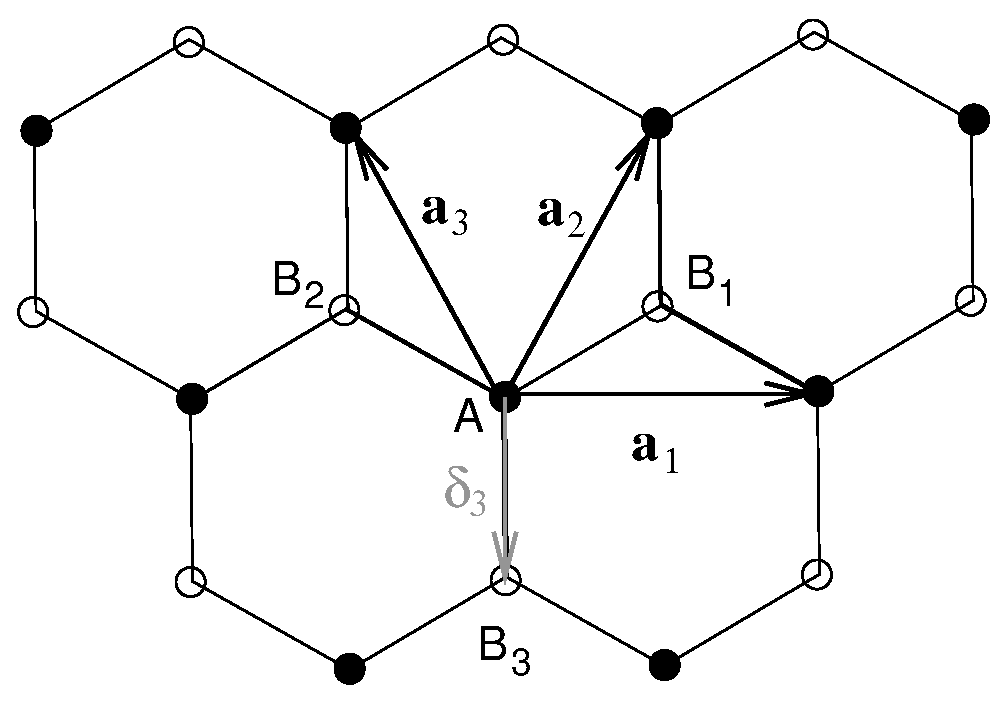
\includegraphics[width=6.5cm,angle=0]{honeycomblattice2.eps}
\caption{蜂巢晶格的紧束缚模型。}
\label{fig2:01}
\end{figure}

接下来,我们忽略近邻格点的波函数交叠,因此交叠矩阵(\ref{eq2:10}),考虑到对波函数的归一化,可以写成$\bone$乘以粒子数$N$。久期方程告诉我们其实能带就是Hamiltonian矩阵(\ref{eq2:09})的本征值。不仅如此,由于两个子格子从化学角度来讲是完全一样的,我们实际上有$\psi_{\bk}^{(A)*}H\psi_{\bk}^{(A)}=\psi_{\bk}^{(B)*}H\psi_{\bk}^{(B)}$,且对角元相当于只对能带贡献一个常数,我们可以取为$0$。因此,(\ref{eq2:09})式中唯一有用的项就是非对角项$\Hmath_{\bk}^{AB}\equiv\psi_{\bk}^{(A)*}H\psi_{\bk}^{(B)} =Nt_{\bk}^{AB}$,其中{\itt hopping项}为
\beq\label{eq2:13}
t_{\bk}^{AB}\equiv \sum_{\bR_l} e^{i\bk\cdot\bR_l}\int d^2r\, 
\phi^{(A)*}(\br-\bR_k) H \phi^{B}(\br+\deltab_{AB}-\bR_m)\ ,
\eeq
而$\deltab_{AB}$是连接A格点和B格点的矢量。
\renewcommand*{\thefootnote}{\fnsymbol{footnote}}

只考虑最近邻格点就足够得到石墨烯的能带结构了,因此其{\itt hopping强度}可以写为
\beq\label{eq2:15}
t\equiv \int d^2r\, \phi^{A*}(\br) H \phi^{B}(\br+\deltab_3),
\eeq
其中取$\deltab_{AB}=\deltab_3$ (见图. \ref{fig2:01}),注意其实也可以考虑远距离的hopping,比如次近邻,这样会产生一些对角项。然而我们知道$t\sim 3$ eV,比次近邻的hopping强度强十倍\cite{antonioRev},而且它只影响低能下石墨烯电子的一些渐进性质\footnote[2]{译者注:会打开能隙,但是很小}。
\renewcommand*{\thefootnote}{\arabic{footnote}}

如果我们考虑任意一个A型子格子上的点$A$(图. \ref{fig2:01}),我们可以看到hopping项(\ref{eq2:13})包含三个最近邻$B_1$,$B_2$和$B_3$,每个都有相同的hopping强度$t$。然而,格点$B_3$与格点$A$用相同的格矢,只不过平移了$\deltab_3$而已,因此在hopping矩阵上并没有相位差;而$B_1$和$B_2$则分别有
\[\ba_2=\frac{\sqrt{3}a}{2}(\be_x + \sqrt{3}\be_y) \qquad{\text{ 和}} \qquad \ba_3\equiv\ba_2-\ba_1=\frac{\sqrt{3}a}{2}(-\be_x + \sqrt{3}\be_y), \]
其中最近邻碳原子间距$a=|\deltab_3|=0.142$ nm。因此,它们分别有相位因子$\exp(i\bk\cdot\ba_2)$和$\exp(i\bk\cdot\ba_3)$,而hopping项(\ref{eq2:13})就可以写为
\[t_{\bk}^{AB}=t\gamma_{\bk}^*=\left(t_{\bk}^{BA}\right)^*,\]
其中,我们对最近邻进行了相位求和
\beq\label{eq2:18}
\gamma_{\bk}\equiv 1+e^{i\bk\cdot\ba_2}+e^{i\bk\cdot\ba_3}.
\eeq

现在能带的色散就可以通过解久期方程(\ref{eq2:11})很容易的得到了
\beq\label{BandDisp}
\epsilon_{\lambda}(\bk) = \lambda\left|t_{\bk}^{AB}\right| = \lambda t\left|\gamma_{\bk}\right|,
\eeq
如图. \ref{fig08}所示。能带色散显然是粒子-空穴对称的,而且价带($\lambda=-$)与导带($\lambda=+$)在两个点接触:
\[\pm \bK= \pm \frac{4\pi}{3\sqrt{3}a}\be_x\ , \]
其具体位置是通过$\gamma_{\pm \bK}=0$来得到的,恰好与BZ的两个角$K$和$K'$一致。在第\ref{zeroB}节中我们讲过,未掺杂的石墨烯的能带结构是半满的,因此费米能恰好处在$K$,$K'$这些点上。


\section*{Continuum Limit\\\bf 连续极限}

低能电子的特性可以通过在$K$和$K'$这样的点附近把能带中的相位因子(\ref{eq2:18})展开而得到
\beqn\label{eq2:30}
\nn
\gamma_{\bp}^{\pm}\equiv \gamma_{\bk=\pm \bK+\bp} &=& 1 + e^{\pm i\bK\cdot\ba_2}
e^{i\bp\cdot\ba_2} + e^{\pm i\bK\cdot\ba_3}e^{i\bp\cdot\ba_3}
\\
\nn
&\simeq& 1 + e^{\pm i 2\pi/3}\left[1 + i\bp\cdot\ba_2\right] + e^{\mp i 2\pi/3}\left[1 + i\bp\cdot\ba_3 \right] \\
\nn
&=& \gamma_{\bp}^{\pm (0)}+\gamma_{\bp}^{\pm (1)}
\eeqn
根据Dirac点的定义和其处于第一BZ的角上$K$和$K'$处,我们有$\gamma_{\bp}^{\pm (0)}=\gamma_{\pm\bK}=0$。做$|\bp|a$为小量的一级展开;方便起见,假定$\hbar=1$,从而动量和波矢有相同的量纲。

一阶展开为
\beqn\label{eq2:31}
\nn
\gamma_{\bp}^{\pm (1)} &=& i\frac{\sqrt{3}a}{2}\left[(p_x+\sqrt{3}p_y)e^{\pm i2\pi/3}
+ (-p_x+\sqrt{3}p_y)e^{\mp i2\pi/3} \right]\\
&=& \mp \frac{3a}{2}(p_x \pm i p_y),
\eeqn
其中利用了$\sin(\pm 2\pi/3)=\pm \sqrt{3}/2$,和$\cos(\pm 2\pi/3)=-1/2$。这导致了有效低能Hamiltonian
\beq\label{eq2:32}
H_{\bp}^{\xi}=\xi v(p_x\sigma^x + \xi p_y\sigma^y),
\eeq
其中费米速度
\beq\label{eq2:32b}
v \equiv \frac{3ta}{2\hbar}\ .
\eeq
其中$\xi=\pm $指的是$K$和$K'$的区分;$K$点的Dirac Hamiltonian可以通过(\ref{0BHams})得到
\beq\label{DirHamK}
H_D=v\bp\cdot\sigmab\, ,
\eeq
而$K'$点的低能Hamiltonian为
\beq\label{DirHamKp}
H_D^{\prime}=-v\bp\cdot\sigmab^*\, ,
\eeq
而其中$\sigmab^*=(\sigma^x,-\sigma^y)$。两种Hamiltonian都给出相同的能谱,因此是{\itt 二重谷简并}的。

注意到,如果为了避免(\ref{DirHamKp})中Hamiltonian的共轭,可以通过交换A和B子格子,而在$K$ ($\xi=+$)和$K'$ ($\xi=-$)两个谷的时候Hamiltonian可以写成这种简略的形式
\beq\label{DirHamBis}
H_D^{\xi}=\xi H_D=\xi v\bp\cdot\sigmab\, .
\eeq


\chapter[有质量的Dirac粒子的Landau能级]{Landau Levels of Massive Dirac Particles\\\bf 有质量的Dirac粒子的Landau能级}
\label{MassLL}


\markboth{Appendix}{Landau Levels of Massive Dirac Particles}


\section*{Mass Confinement of Dirac Fermions at $B=0$\\\bf Dirac费米子在$B=0$下的质量限制}

即使不存在磁场的时候,石墨烯中对电子的约束也是很微妙的,因为构造一个简单的$V_{\rm conf}=V(y)\bone$这样的束缚势能是不能束缚Dirac电子的。这是由于叫{\itt Klein悖论}的相对论性效应导致的,即一个(无质量的)相对论性粒子可以穿透势垒而不产生背向散射\cite{klein}。这种效应可以这么理解:考虑入射的电子处于$V=0$状态,而电子的能量比费米能稍微高一点。在势垒处,Dirac点被提高到了很高的能量,而这里的Fermi能处于价带。
This effect may be understood in the following manner: consider an incident electron in the region with $V=0$ the
energy of which is slightly above the Fermi energy. In the potential barrier, the Dirac point is shifted to a higher
energy that corresponds to the barrier height and the Fermi energy lies now in the valence band, where the electron
may still find a quantum state (with the same wave-vector direction and the same velocity $v$) -- instead of 
moving as an electron in the conduction band, it thus simply moves in the same direction as an electron in the valence
band [图. \ref{fig2:02}(a)]. This is in stark contrast with quantum mechanical tunneling of a non-relativistic particle,
for which the transmission probability through a potential barrier is exponentially suppressed because of a lacking
quantum state at the same energy as that of the incident electron. 


\begin{figure}
\centering
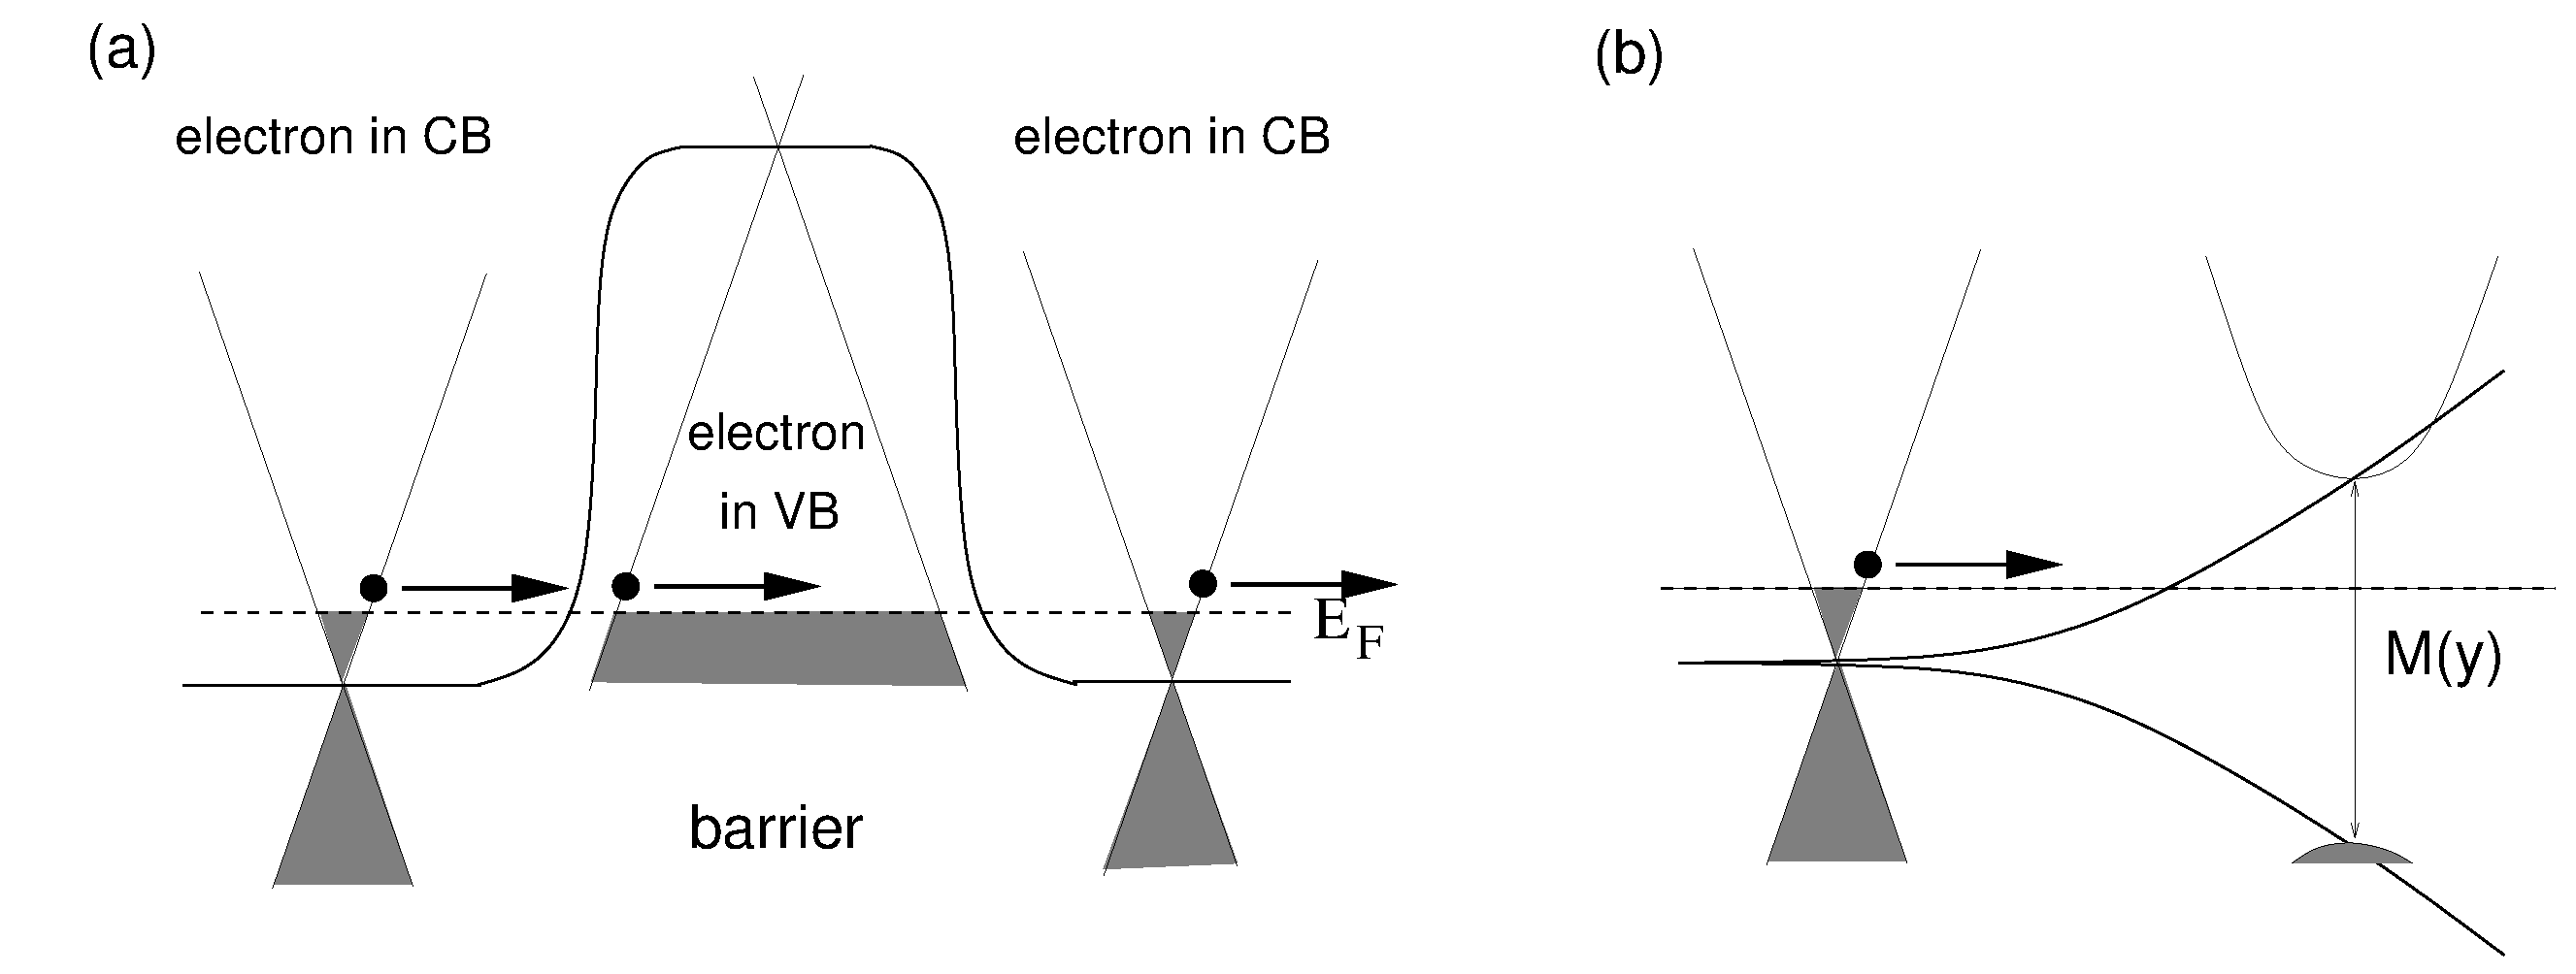
\includegraphics[width=12cm,angle=0]{KleinTunneling.eps}
\caption{ {\sl (a)} Klein tunneling through a barrier. An incident electron in the conduction band (CB) above the Fermi energy, 
which is at the Dirac point before the barrier, transverses the barrier as en electron above the Fermi energy in the valence band (VB).
The valence band is partially emptied because the Dirac point has shifted to a higher energy corresponding to the barrier height.
{\sl (b)} Mass confinement. A gap opens when the particle approaches the edge, which becomes a forbidden region
where no quantum state can be found at the energy corresponding to that of the incident electron.}
\label{fig2:02}
\end{figure}


The problem is circumvented by a so-called {\sl mass confinement}
\beq\label{MassConfA}
V_{\rm conf}=V(y)\,\sigma^z=\left(\begin{array}{cc} V(y) & 0 \\ 0 & -V(y) \end{array}\right),
\eeq
and we discuss first the simpler case of a constant mass term $M\sigma^z$ that needs to be added to the Dirac 
Hamiltonian. That this term yields indeed a mass may be seen from the Dirac Hamiltonian at $B=0$ 
\beq\label{MassDir}
H_D^m=v\bp\cdot\sigmab + M\sigma^z=\left(
\begin{array}{cc}
 M & v(p_x - ip_y) \\ v(p_x + ip_y) & -M
\end{array}\right),
\eeq 
the diagonalisation of which yields the energy spectrum
$$\epsilon_{\lambda}(\bp)= \lambda\sqrt{v^2|\bp|^2 + M^2},$$
which is gapped at zero momentum. This is nothing other than the dispersion relation of a relativistic particle\footnote{
The sign $\lambda=-$ corresponds to the anti-particle.}
with mass $m$ such that $M=mv^2$. Qualitatively one may see from 图. \ref{fig2:02}(b) why a mass confinement is 
more efficient than a potential barrier. Indeed, when the particle approaches the edge with $M(y)\neq 0$ a gap opens. 
An electron slightly above the Dirac point may then only propagate in the region with $M=0$, whereas at the edge its
energy lies in the gap which is a forbidden region, and the electron is thus confined. 

Similarly to the $B=0$ case, one may find the energy spectrum of the massive Dirac Hamiltonian (\ref{MassDir}) in 
a perpendicular magnetic field, which reads, in terms of the ladder operators $a$ and $a^{\dagger}$,
\beq\label{MassDirB}
H_D^B=  \left(\begin{array}{cc}
M & v(\Pi_x- i \Pi_y) \\ v(\Pi_x+ i \Pi_y) & -M
        \end{array}\right) = \left(\begin{array}{cc}
M & \sqrt{2}\frac{\hbar v}{l_B} a \\ \sqrt{2}\frac{\hbar v}{l_B} a^{\dagger} & -M
        \end{array}\right) .
\eeq
Its eigenvalues may be obtained in the same manner as in the $M=0$ case (c.f. Sec. \ref{RelLLsec}), and one obtains
\beq\label{MassiveLL}
\epsilon_{\lambda n} = \lambda \sqrt{M^2 + 2\frac{\hbar^2 v^2}{l_B^2} n} 
\eeq
for the massive relativistic LLs, $n\neq 0$. 

Special care needs to be taken in the discussion of the central LL $n=0$, which necessarily shifts away from zero energy.
The associated quantum state (\ref{spinN0}) is zero in the first component $u_0$, whereas the second component is 
given by $v_0=|0\rangle$. In order to satisfy the second line in the eigenvalue equation 
$$
H_D^B \psi_0 = \epsilon_0 \psi_0 \qquad {\Leftrightarrow} \qquad
\left(\begin{array}{cc}
M & \sqrt{2}\frac{\hbar v}{l_B} a \\ \sqrt{2}\frac{\hbar v}{l_B} a^{\dagger} & -M
        \end{array}\right)\left(\begin{array}{c} 0 \\ |0\rangle \end{array}\right) 
= \epsilon _0 \left(\begin{array}{c} 0 \\ |0\rangle \end{array}\right) ,
$$
one needs to fulfil 
\beq\label{CondMass}
\sqrt{2}\frac{\hbar v}{l_B}\, a^{\dagger}\, u_0 = (\epsilon_0 + M) v_0 \qquad \Leftrightarrow \qquad
0=(\epsilon_0 + M)|0\rangle,
\eeq
such that the only solution is $\epsilon_0 = -M$. The relativistic $n=0$ LL is therefore shifted to negative energies
and does no longer satisfy particle-hole symmetry. This effect is called {\sl parity anomaly} and depends
on the {\sl sign of the mass}. 

In the case of graphene, we need to remember that there are two copies of the energy spectrum, one at the $K$ point
and one at the $K'$ point. As we have disussed in Appendix \ref{TBgraphene}, the Hamiltonian (\ref{MassDirB}) describes
the low-energy properties at the $K$ point whereas we need to interchange the A and B sublattices at the $K'$ point and add
a global sign in front of the off-diagonal terms [see Eq. (\ref{DirHamBis})],
\beq\label{MassDirBp}
H_D^{B\prime}=   \left(\begin{array}{cc}
- M & - \sqrt{2}\frac{\hbar v}{l_B} a \\ -\sqrt{2}\frac{\hbar v}{l_B} a^{\dagger} & M
        \end{array}\right) = -H_D^{B\prime}.
\eeq
Naturally, the eigenstates of this Hamiltonian are the same as those of the Hamiltonian (\ref{MassDirB}) at the 
$K$ point, but the eigenvalues change their sign. Due to the particle-hole symmetry of the levels (\ref{MassiveLL}),
the global sign does not affect the energy spectrum for $n\neq 0$. However, the $n=0$ LL, which
does not respect particle-hole symmetry, must again be treated apart, and one finds in the same manner as for the $K$ point
the condition corresponding to Eq. (\ref{CondMass}),
\beq\label{CondMassbis}
-\sqrt{2}\frac{\hbar v}{l_B}\, a^{\dagger}\, u_0 = (\epsilon_0 - M) v_0 \qquad \Leftrightarrow \qquad
0=(\epsilon_0 - M)|0\rangle.
\eeq
One notices that the $n=0$ LL level at the $K'$ point shifts to positive energies as a function of the mass, such that 
the overall level spectrum for graphene, when one takes into account {\sl both} valleys, 
is again particle-hole symmetric, but the valley degeneracy is lifted for
$n=0$.

The case of a mass term that varies in the $y$-direction, such as for the mass confinement potential, may finally
be treated in the same manner as we have discussed in Sec. \ref{secInv}: the system remains translation-invariant in
the $x$-direction, such that the Landau gauge is the appropriate gauge and the wave vector $k$ in this direction
is a good quantum number. Because this wave vector determines the position of the eigenstate in the $y$-direction,
$y_0=kl_B^2$, the energy spectrum is given by the expression (\ref{MassSpec}),
\beq\label{MassSpecA}
\epsilon_{\lambda n,y_0;\xi} = \lambda \sqrt{M^2(y_0) + 2\frac{\hbar^2 v^2}{l_B^2} n}, 
\eeq
for $n\neq 0$ and both valleys $\xi=\pm$, whereas the $n=0$ LL is found at 
\beq\label{MassSpec0}
\epsilon_{n=0,y_0;\xi} = -\xi M(y_0).
\eeq



\clearpage
%\iffalse


\markboth{Bibliography}{Bibliography}



\bibliographystyle{cj} 
\bibliography{refsQHE} 

%\fi

\end{document}
